% Lärguide till valuation-engine.
% Bygg: ./build.sh   (kräver tectonic)
\documentclass[10pt,a4paper,titlepage=true]{scrartcl}
% Preamble for the study guide. Built with tectonic (XeTeX engine).
\usepackage{amsmath}
\usepackage{mathtools}
\usepackage[mono=false]{libertinus}
\usepackage{fontspec}
\setmonofont{DejaVuSansMono.ttf}[
  Scale=0.80,
  HyphenChar=None,
  BoldFont=DejaVuSansMono-Bold.ttf,
  ItalicFont=DejaVuSansMono-Oblique.ttf,
  BoldItalicFont=DejaVuSansMono-BoldOblique.ttf]
\usepackage{polyglossia}
\setdefaultlanguage{swedish}
\setotherlanguage{english}
\usepackage[a4paper,left=2.5cm,right=2.5cm,top=2.3cm,bottom=2.6cm,footskip=1.1cm]{geometry}
\usepackage{microtype}
\usepackage{xcolor}
\usepackage{graphicx}
\usepackage{booktabs}
\usepackage{tabularx}
\usepackage{array}
\usepackage{multicol}
\usepackage{enumitem}
\usepackage{siunitx}
\usepackage{float}
\usepackage{listings}
\usepackage{tikz}
\usetikzlibrary{arrows.meta,positioning,fit,calc}
\usepackage[most]{tcolorbox}
\usepackage[hidelinks,unicode,bookmarksnumbered,bookmarksopen,bookmarksopenlevel=1]{hyperref}
\usepackage{bookmark}

\graphicspath{{../figures/}}

% ---------------------------------------------------------------- colours
\definecolor{accent}{HTML}{1F4E79}
\definecolor{boxblue}{HTML}{1F5FA8}
\definecolor{boxred}{HTML}{B5402F}
\definecolor{boxgreen}{HTML}{217A52}
\definecolor{boxgray}{HTML}{5F6670}
\definecolor{codebg}{HTML}{F5F6F8}
\definecolor{codeframe}{HTML}{D4D8DE}
\definecolor{codegray}{HTML}{6A737D}
\definecolor{codeblue}{HTML}{1F4E79}
\definecolor{codegreen}{HTML}{2D6A4F}

% ---------------------------------------------------------------- KOMA
\KOMAoptions{parskip=half-,headings=small,captions=tableheading,toc=flat}
\DeclareTOCStyleEntries[raggedentrytext=true]{tocline}{section,subsection}
\setkomafont{disposition}{\sffamily\bfseries\color{accent}}
\setkomafont{title}{\sffamily\bfseries\color{accent}}
\setkomafont{subtitle}{\sffamily\color{black!70}}
\setkomafont{caption}{\small}
\setkomafont{captionlabel}{\small\sffamily\bfseries\color{accent}}
\setcapindent{0pt}
\addtokomafont{descriptionlabel}{\rmfamily\bfseries}
\RedeclareSectionCommand[beforeskip=1.6\baselineskip,afterskip=0.6\baselineskip]{section}
\RedeclareSectionCommand[beforeskip=1.0\baselineskip,afterskip=0.3\baselineskip]{subsection}
\RedeclareSectionCommand[beforeskip=0.7\baselineskip,afterskip=0.15\baselineskip]{subsubsection}
\addtokomafont{section}{\Large}
% Little stretch between paragraphs: with the default (plus half a line) a ragged-bottom page
% can be cut short at any heading, which leaves large gaps at the foot of the page.
\setparsizes{0pt}{0.5\baselineskip plus 0.6pt}{0pt plus 1fil}
\setlength{\textfloatsep}{14pt plus 2pt minus 2pt}
\setlength{\intextsep}{12pt plus 2pt minus 2pt}
\setlength{\floatsep}{12pt plus 2pt minus 2pt}
\setcounter{secnumdepth}{2}
\setcounter{tocdepth}{2}
\numberwithin{equation}{section}
\numberwithin{figure}{section}
\numberwithin{table}{section}
\renewcommand{\floatpagefraction}{0.8}
\renewcommand{\topfraction}{0.9}
\renewcommand{\bottomfraction}{0.7}
\renewcommand{\textfraction}{0.08}
\setlength{\emergencystretch}{2em}
\setlist{itemsep=0.15em,topsep=0.3em,parsep=0pt,leftmargin=1.6em}
\setlist[description]{leftmargin=1.6em,labelindent=0pt}

% ---------------------------------------------------------------- decimal comma
% Same behaviour as the icomma package (a comma followed by a space is punctuation,
% otherwise a decimal comma), but set up after unicode-math so that the comma glyph
% comes from the math font in use.
\makeatletter
\AtBeginDocument{%
  \Umathcharnumdef\mathcomma=\Umathcodenum`\,\relax
  \mathcode`\,="8000\relax}
\begingroup\catcode`\,=\active
  \gdef,{\futurelet\@let@token\sm@rtcomma}
\endgroup
\def\sm@rtcomma{%
  \ifx\@let@token\@sptoken\else\ifx\@let@token\space\else\mathord\fi\fi\mathcomma}
\makeatother

% ---------------------------------------------------------------- numbers
\sisetup{output-decimal-marker={,},group-separator={\,},group-minimum-digits=4,
         detect-all,mode=match}
\newcommand{\pct}{\,\%}
\newcommand{\kr}{\,kr}
\newcommand{\x}{\ensuremath{\times}}          % "19,4\x" = 19,4 times

% ---------------------------------------------------------------- text macros
\newcommand{\eng}[1]{(\textenglish{\emph{#1}})}
\newcommand{\en}[1]{\textenglish{\emph{#1}}}
\newcommand{\kod}[1]{\texttt{\detokenize{#1}}}
\newcommand{\flag}[1]{\texttt{-{}-\detokenize{#1}}}   % command line flag
\newcommand{\EV}{\mathrm{EV}}
\newcommand{\TV}{\mathrm{TV}}
\newcommand{\FCFF}{\mathrm{FCFF}}
\newcommand{\FCFE}{\mathrm{FCFE}}
\newcommand{\EBITDA}{\mathrm{EBITDA}}
\newcommand{\EBIT}{\mathrm{EBIT}}
\newcommand{\NOPAT}{\mathrm{NOPAT}}
\newcommand{\WACC}{\mathrm{WACC}}
\newcommand{\ERP}{\mathrm{ERP}}
\newcommand{\NWC}{\mathrm{NWC}}
\newcommand{\PV}{\mathrm{PV}}
\newcommand{\IRR}{\mathrm{IRR}}
\newcommand{\MOIC}{\mathrm{MOIC}}
\newcommand{\Cov}{\operatorname{Cov}}
\newcommand{\Var}{\operatorname{Var}}
\newcommand{\E}{\operatorname{E}}
\newcommand{\T}{^{\mathsf{T}}}

% ---------------------------------------------------------------- callouts
\newtcolorbox{callout}[2]{enhanced,breakable=false,colback=#1!5!white,colframe=#1,
  boxrule=0pt,leftrule=3pt,arc=0pt,outer arc=0pt,left=8pt,right=8pt,top=5pt,bottom=5pt,
  before skip=0.8\baselineskip,after skip=0.8\baselineskip,
  fonttitle=\sffamily\bfseries\small,coltitle=#1,colbacktitle=#1!5!white,
  title={#2},attach title to upper={\quad},parbox=false}
\newenvironment{komihag}{\begin{callout}{boxblue}{Kom ihåg}}{\end{callout}}
\newenvironment{vanligtfel}{\begin{callout}{boxred}{Vanligt fel}}{\end{callout}}
\newenvironment{intervjutips}{\begin{callout}{boxgreen}{Intervjutips}}{\end{callout}}
\newenvironment{imotorn}{\begin{callout}{boxgray}{Så gör motorn}}{\end{callout}}

% ---------------------------------------------------------------- listings
\lstdefinestyle{base}{basicstyle=\ttfamily\small,columns=fullflexible,keepspaces=true,
  backgroundcolor=\color{codebg},frame=single,rulecolor=\color{codeframe},framerule=0.4pt,
  xleftmargin=6pt,xrightmargin=6pt,framesep=5pt,aboveskip=0.7\baselineskip,
  belowskip=0.5\baselineskip,showstringspaces=false,breaklines=true,breakatwhitespace=true,
  upquote=true,literate={-}{{-}}1}
\lstdefinestyle{py}{style=base,language=Python,keywordstyle=\color{codeblue}\bfseries,
  commentstyle=\color{codegray}\itshape,stringstyle=\color{codegreen}}
\lstdefinestyle{sh}{style=base,language=bash,keywordstyle=\color{black},
  commentstyle=\color{codegray}\itshape,stringstyle=\color{black}}
\lstdefinestyle{txt}{style=base,language={}}
\lstset{style=py}
\AtBeginDocument{\renewcommand{\lstlistingname}{Kodexempel}}

% ---------------------------------------------------------------- Q&A and exercises
\newcounter{fraga}
\newenvironment{fraga}[1]{\par\addvspace{0.9\baselineskip}\refstepcounter{fraga}%
  \noindent\begin{minipage}{\linewidth}\setlength{\parskip}{0.4\baselineskip plus 0.6pt}%
  \noindent\textsf{\textbf{\color{accent}Q\thefraga.}}\enspace\textenglish{\textbf{#1}}\par
  \noindent\ignorespaces}{\end{minipage}\par}
\newcommand{\fraser}[1]{\par\noindent{\small\textsf{\textbf{Säg på engelska:}}
  \textenglish{\itshape #1}}\par}
\newcounter{ovning}
\newenvironment{ovning}[1][]{\par\refstepcounter{ovning}\addvspace{0.8\baselineskip}%
  \noindent\textsf{\textbf{\color{accent}Övning \theovning}}%
  \if\relax\detokenize{#1}\relax\else\ \textsf{(#1)}\fi\textsf{\textbf{.}}\enspace}{\par}
\newenvironment{losning}{\par\vspace{0.2\baselineskip}\noindent\textsf{\textbf{Lösning.}}\enspace}{\par}


\hypersetup{
  pdftitle={Värdering i praktiken: lärguide till valuation-engine},
  pdfauthor={valuation-engine},
  pdfsubject={DCF, multipelvärdering, LBO och Monte Carlo på svenska börsbolag},
  pdflang={sv}}

\begin{document}
% Hyphenation exceptions (set here so that they apply to Swedish, the document language).
\hyphenation{EBITDA EBIT WACC NOPAT FCFF FCFE MOIC Yahoo aktie-ägare aktie-ägarna
  aktie-ägarnas lån-givare lån-givarna åter-investerar ut-låning där-utöver}

\begin{titlepage}
  \thispagestyle{empty}
  \vspace*{3.2cm}
  {\color{accent}\rule{\linewidth}{2.2pt}}\par
  \vspace{0.9cm}
  {\sffamily\bfseries\color{accent}\fontsize{32}{38}\selectfont Värdering i praktiken\par}
  \vspace{0.6cm}
  {\sffamily\fontsize{15}{20}\selectfont\color{black!75}
   Lärguide till \texttt{valuation-engine}: DCF, multiplar, LBO och Monte Carlo\\
   på svenska börsbolag, med Atlas Copco som genomgående exempel\par}
  \vspace{0.9cm}
  {\color{accent}\rule{\linewidth}{0.6pt}}\par
  \vspace{1.2cm}
  {\large För dig som kan matematiken men är ny på företagsvärdering\\
   och siktar på investment banking.\par}
  \vfill
  {\sffamily\large valuation-engine\par}
  \vspace{0.2cm}
  {\sffamily 16 november 2026\par}
  \vspace{1.2cm}
  {\small\color{black!65} Guiden är ett läromedel och ingen investeringsrådgivning. Alla tal om
   Atlas Copco kommer från projektets egen körning på data från Yahoo Finance (kurs per den
   13 november 2026, bokslut 2025) och är inte avstämda mot bolagets årsredovisning.\par}
\end{titlepage}

\pdfbookmark[1]{Innehåll}{toc}
\section*{Innehåll}
\begingroup
  \small\setlength{\columnsep}{2.2em}\setlength{\parskip}{0pt}
  \begin{multicols}{2}
    \makeatletter\@starttoc{toc}\makeatother
  \end{multicols}
\endgroup
\clearpage

\section{Översikt: vad en investmentbank gör och var värdering kommer in}
\label{sec:oversikt}

Du kan redan räkna. Det du behöver lära dig är vad som ska räknas, varför, och hur man pratar om
det. Den här guiden går igenom de fyra värderingsmetoder som en junior på en investmentbank
förväntas kunna, och den gör det med ett riktigt program som facit: \kod{valuation-engine}, som
värderar alla svenska bolag på Yahoo Finance. Varje påstående om vad programmet gör är
kontrollerat mot koden, och alla tal om Atlas Copco kommer från en och samma körning.

\subsection{Vad en investmentbank gör}

En investmentbank \eng{investment bank} tjänar pengar på rådgivning och kapitalanskaffning, inte
på in- och utlåning. Verksamheten brukar delas upp så här:

\begin{description}
  \item[Företagsaffärer] \eng{mergers and acquisitions, M\&A}. Banken ger råd till den som säljer
    ett bolag (säljuppdrag, \en{sell-side}) eller den som köper (köpuppdrag, \en{buy-side}).
    Arvodet är oftast en andel av affärens värde.
  \item[Aktiemarknad] \eng{equity capital markets, ECM}. Börsintroduktioner \eng{initial public
    offering, IPO} och nyemissioner.
  \item[Skuldmarknad] \eng{debt capital markets, DCM}. Obligationer och lån, bland annat
    finansieringen av lånefinansierade uppköp \eng{leveraged finance}.
\end{description}

Som analytiker \eng{analyst}, den första rollen efter examen, bygger du modeller i Excel och
sidor i PowerPoint. Nästan allt du gör vilar på en fråga: \emph{vad är bolaget värt, och varför?}

\subsection{Var värderingen används}

\begin{description}
  \item[Pitch.] Banken försöker vinna ett uppdrag och visar i en presentation \eng{pitch book} vad
    den tror att bolaget är värt. Slutbilden är ofta ett diagram med ett värdeintervall per
    metod, en så kallad \en{football field} (figur~\ref{fig:football} på
    sidan~\pageref{fig:football}).
  \item[Fairness opinion.] Ett skriftligt utlåtande till en styrelse om att ett bud är skäligt ur
    finansiell synvinkel. Här ska varje antagande tåla granskning.
  \item[M\&A.] Köparen vill veta vad den högst kan betala, säljaren vad den minst bör godta.
    Diskonterade kassaflöden ger ett fristående värde, jämförelsebolag visar vad marknaden
    betalar i dag.
  \item[LBO.] När köparen är ett riskkapitalbolag \eng{private equity} räknar man baklänges: vilket
    pris ger ägaren den avkastning den kräver? Det priset fungerar ofta som ett golv i
    budgivningen, eftersom en finansiell köpare saknar synergier.
\end{description}

Ingen metod ger ett sant värde. Poängen med att använda flera är att se \emph{var} de skiljer sig
och kunna förklara varför. Det är också vad kapitel~\ref{sec:case} handlar om: metoderna säger
116 till 178\kr{} per aktie för Atlas Copco när kursen är 192,25\kr, och det intressanta är
förklaringen.

\subsection{Projektet mot verkligheten}

Tabell~\ref{tab:mappning} visar vad varje del av projektet motsvarar på en bank, och var
projektet förenklar. Läs högerkolumnen noga: det är de sakerna en intervjuare frågar om.

\begin{table}[ht]
\centering\small
\caption{Projektets delar och vad de motsvarar i arbetet på en bank.}
\label{tab:mappning}
\begin{tabularx}{\linewidth}{@{}l>{\raggedright\arraybackslash}X>{\raggedright\arraybackslash}X@{}}
\toprule
Del av projektet & Motsvarar på banken & Viktigaste förenklingen \\
\midrule
\kod{data/} & Att hämta bokslut och kurser ur årsredovisningar och betalda databaser och
  justera dem för hand & Gratis data från Yahoo Finance, mekanisk mappning, senaste räkenskapsår
  i stället för rullande tolv månader \\
\kod{models/dcf.py} & DCF-modellen i Excel & Prognosen räknas mekaniskt ur tre till fyra års
  historik, ingen analytiker har läst bolagets rapporter \\
\kod{models/comps.py} & Jämförelsebolagsanalys \eng{trading comps} & Jämförelsebolagen väljs
  av en algoritm, inte av någon som kan branschen \\
\kod{models/lbo.py} & LBO-modellen & Årsmodell med två lånetrancher och schablonvillkor \\
\kod{models/monte_carlo.py} & Känslighetsanalysen. Banker visar oftast tabeller, simulering är
  ovanligare i pitchmaterial & Fyra drivare, antagna standardavvikelser \\
\kod{viz/} & Diagrammen i presentationen & Samma diagram för alla bolag \\
\kod{export/excel.py} & Själva modellen, som på en bank lever i Excel & En export med
  färdiga tal, bara ett fåtal levande formler \\
\kod{batch.py} & Screening av många bolag & Ingen manuell kontroll per bolag \\
\bottomrule
\end{tabularx}
\end{table}

\begin{komihag}
Motorn är konsekvent, inte klok. Den gör samma sak med alla 687 bolag och kraschar inte, men
den vet ingenting om bolagen. Det du ska lära dig av den är mekaniken och var omdömet behövs.
\end{komihag}

\subsection{Beteckningar}

Samma symboler används i hela guiden. Belopp anges i miljarder kronor (mdkr) om inget annat
sägs, och räntor som decimaltal i formler och procent i text.

\begin{table}[ht]
\centering\small
\caption{Beteckningar.}
\label{tab:beteckningar}
\begin{tabularx}{\linewidth}{@{}lX@{\hspace{1.5em}}lX@{}}
\toprule
Symbol & Betydelse & Symbol & Betydelse \\
\midrule
$t$ & år, $t = 1, \dots, N$ & $r$ & diskonteringsränta, i DCF lika med $\WACC$ \\
$N$ & antal prognosår (5 i motorn) & $g$ & evig tillväxt \eng{terminal growth} \\
$R_t$ & omsättning år $t$ & $r_f$ & riskfri ränta \\
$m$ & EBITDA-marginal & $\ERP$ & aktiemarknadens riskpremie \\
$d$, $c$ & avskrivningar respektive capex som andel av omsättningen & $\beta_L$, $\beta_U$ &
  beta med respektive utan skuldsättning \\
$\nu$ & rörelsekapital som andel av omsättningen & $r_e$, $r_d$ & avkastningskrav på eget
  kapital respektive låneränta före skatt \\
$\tau$ & skattesats (20,6\pct{} i projektet) & $E$, $D$ & marknadsvärde på eget kapital
  respektive skuld \\
$\FCFF_t$ & fritt kassaflöde till alla finansiärer & $\TV_N$ & slutvärde vid utgången av år
  $N$ \\
$\EV$ & rörelsevärde \eng{enterprise value} & $M$ & multipel, till exempel $\EV/\EBITDA$ \\
\bottomrule
\end{tabularx}
\end{table}

\section{Redovisningen du behöver}
\label{sec:redovisning}

Värdering börjar i bokslutet. Du behöver inte kunna bokföra, men du måste kunna läsa de tre
rapporterna och veta hur en ändring i en av dem slår igenom i de andra två. Talen i exemplen är
Atlas Copcos för 2025 så som datalagret levererar dem, i mdkr.

\subsection{De tre rapporterna}

\begin{description}
  \item[Resultaträkningen] \eng{income statement} visar intäkter och kostnader under ett år.
    Den är periodiserad: en kostnad tas när resursen förbrukas, inte när den betalas.
  \item[Balansräkningen] \eng{balance sheet} visar vad bolaget äger och hur det är finansierat
    en viss dag. Den ska alltid gå ihop:
    $\text{tillgångar} = \text{skulder} + \text{eget kapital}$.
  \item[Kassaflödesanalysen] \eng{cash flow statement} visar vart pengarna faktiskt tog vägen
    under året, uppdelat på löpande verksamhet, investeringar och finansiering.
\end{description}

\begin{table}[ht]
\centering\small
\caption{Resultaträkningens trappa, Atlas Copco 2025 (mdkr). Källa: projektets datalager.}
\label{tab:rr}
\begin{tabular}{@{}llr@{}}
\toprule
Rad & Engelska & 2025 \\
\midrule
Omsättning & \en{revenue}, \en{sales} & 168,3 \\
$-$ Kostnad för sålda varor & \en{cost of goods sold, COGS} & 96,1 \\
$=$ Bruttoresultat & \en{gross profit} & 72,2 \\
$-$ Övriga rörelsekostnader (före avskrivningar) & \en{operating expenses} & 28,1 \\
$=$ \textbf{EBITDA} & & 44,1 \\
$-$ Avskrivningar & \en{depreciation and amortization, D\&A} & 9,5 \\
$=$ \textbf{EBIT}, rörelseresultat & \en{operating income} & 34,6 \\
$-$ Räntekostnader & \en{interest expense} & 0,9 \\
$=$ Resultat före skatt & \en{pretax income, EBT} & 33,7 \\
$-$ Skatt & \en{income tax} & 7,2 \\
$=$ Nettoresultat & \en{net income} & 26,4 \\
\bottomrule
\end{tabular}
\end{table}

Balansräkningen samma år: tillgångar 202,5, skulder 92,1, eget kapital hänförligt till
aktieägarna 110,2 och minoritetens andel 0,2. Kassaflödet från den löpande verksamheten var
32,6, investeringarna i anläggningar (capex) 6,2 och utdelningen 14,6.

\paragraph{Hur de hänger ihop.} Figur~\ref{fig:tre-rapporter} visar kopplingarna. Lär dig dem som
en kedja:

\begin{enumerate}
  \item Nettoresultatet är första raden i kassaflödesanalysen och ökar det egna kapitalet
    (balanserade vinstmedel, \en{retained earnings}), minus utdelning.
  \item Avskrivningar är en kostnad utan utbetalning. De läggs tillbaka i kassaflödet och minskar
    anläggningstillgångarna i balansräkningen.
  \item Investeringar (capex) syns inte i resultaträkningen. De är ett utflöde i kassaflödet och
    ökar anläggningstillgångarna.
  \item Ökat rörelsekapital binder pengar: ett utflöde i kassaflödet, en ökning av
    omsättningstillgångarna i balansräkningen.
  \item Summan av de tre kassaflödena är årets förändring av kassan, som är en rad i
    balansräkningen. Där sluts cirkeln.
\end{enumerate}

\begin{figure}[ht]
\centering
\begin{tikzpicture}[font=\small\sffamily,
  box/.style={draw=accent,rounded corners=2pt,align=left,inner sep=5pt,text width=3.9cm,
              fill=accent!4},
  head/.style={font=\small\sffamily\bfseries,text=accent},
  link/.style={-{Stealth[length=5pt]},thick,draw=black!60},
  lbl/.style={font=\footnotesize\sffamily,fill=white,inner sep=1.5pt,text=black!75}]
  \node[box] (rr) {\textbf{Resultaträkning}\\ Omsättning\\ EBITDA\\ $-$ Avskrivningar\\ EBIT\\
    $-$ Ränta, skatt\\ \textbf{Nettoresultat}};
  \node[box,right=1.5cm of rr] (kf) {\textbf{Kassaflödesanalys}\\ Nettoresultat\\
    $+$ Avskrivningar\\ $-$ Ökning rörelsekapital\\ $-$ Capex\\ $\pm$ Lån, utdelning\\
    \textbf{Förändring av kassa}};
  \node[box,right=1.5cm of kf] (br) {\textbf{Balansräkning}\\ Kassa\\ Rörelsekapital\\
    Anläggningstillgångar\\ Skulder\\ Eget kapital\\ \emph{(tillgångar = skulder + EK)}};
  \draw[link] (rr.east) to node[lbl,above=1pt] {resultat} (kf.west);
  \draw[link] (kf.east) to node[lbl,above=1pt] {kassa} (br.west);
  \draw[link] (rr.south) to[out=-90,in=-90,looseness=0.42]
    node[lbl,pos=0.5] {nettoresultat ökar eget kapital, avskrivningar minskar anläggningstillgångar}
    (br.south);
\end{tikzpicture}
\caption{De tre rapporterna och hur de hänger ihop.}
\label{fig:tre-rapporter}
\end{figure}

\subsection{EBITDA}

EBITDA \eng{earnings before interest, taxes, depreciation and amortization} är rörelseresultatet
före avskrivningar. Måttet är populärt av tre skäl. Det påverkas inte av hur bolaget är
finansierat (räntan ligger längre ned), inte av avskrivningsprinciper, och det är en grov
approximation av kassaflödet från rörelsen före investeringar.

\begin{vanligtfel}
Att behandla EBITDA som kassaflöde. EBITDA tar inte hänsyn till investeringar, bundet
rörelsekapital eller skatt. Två bolag med samma EBITDA kan ha helt olika fritt kassaflöde.
Sedan redovisningsregeln IFRS~16 ligger dessutom hyreskostnader för leasade tillgångar som
avskrivning och ränta, alltså \emph{under} EBITDA. Motorn justerar inte för det, och
kassaflödena under prognosåren blir därför något för höga för bolag med mycket leasing.
\end{vanligtfel}

\subsection{Rörelsekapital}

Rörelsekapital \eng{net working capital, NWC} är de pengar som är bundna i den dagliga
verksamheten. Motorn använder den smala, operativa definitionen:
\begin{equation}
  \NWC = \text{kundfordringar} + \text{lager} - \text{leverantörsskulder}.
  \label{eq:nwc}
\end{equation}
För Atlas Copco 2025: $29,9 + 26,7 - 16,4 = 40,2$~mdkr, eller 23,9\pct{} av omsättningen. När
bolaget växer måste rörelsekapitalet växa med, och den ökningen är ett kassautflöde. I prognosen
antar motorn att rörelsekapitalet är en fast andel $\nu$ av omsättningen, så att
$\Delta\NWC_t = \nu\,(R_t - R_{t-1})$. Ett bolag som får betalt i förskott kan ha negativt
rörelsekapital, och då \emph{frigör} tillväxt pengar.

\subsection{Fritt kassaflöde: FCFF och FCFE}

Fritt kassaflöde är det som blir över när rörelsen har fått sitt. Det finns två varianter, och
skillnaden är vem pengarna tillhör.

\begin{description}
  \item[FCFF] \eng{free cash flow to the firm, unlevered free cash flow} är kassaflödet till
    \emph{alla} finansiärer, långivare och aktieägare, före räntor:
    \begin{equation}
      \FCFF = {\underbrace{\EBIT\,(1-\tau)}_{\NOPAT}} + \text{avskrivningar} - \text{capex}
              - \Delta\NWC .
      \label{eq:fcff}
    \end{equation}
    Skatten räknas som om bolaget saknade skuld. Värdet av ränteavdraget kommer i stället in via
    diskonteringsräntan (avsnitt~\ref{sec:wacc}).
  \item[FCFE] \eng{free cash flow to equity, levered free cash flow} är det som blir kvar till
    aktieägarna sedan långivarna fått sitt:
    \begin{equation}
      \FCFE = \FCFF - \text{ränta}\,(1-\tau) + \text{nettoupplåning}.
      \label{eq:fcfe}
    \end{equation}
\end{description}

Regeln är att kassaflöde och diskonteringsränta måste höra ihop. FCFF diskonteras med WACC och
ger rörelsevärdet. FCFE diskonteras med avkastningskravet på eget kapital och ger aktievärdet
direkt. Motorn räknar bara med FCFF, vilket också är standard på en bank, eftersom man då inte
behöver prognostisera skuldsättningen år för år.

\paragraph{Exempel.} Motorns första prognosår för Atlas Copco (2026): EBITDA 47,10 och
avskrivningar 9,00 ger EBIT 38,11. Skatt 20,6\pct{} på det är 7,85, så $\NOPAT = 30,26$. Capex är
6,09 och rörelsekapitalet ökar med 2,54. Enligt~\eqref{eq:fcff}:
$\FCFF = 30,26 + 9,00 - 6,09 - 2,54 \approx 30,6$~mdkr.

\subsection{Klassikern: avskrivningarna ökar med 10 kronor}
\label{sec:avskrivning10}

Frågan kommer i nästan varje intervju, och den testar om du kan kedjan ovan. Gå alltid i
ordningen resultaträkning, kassaflöde, balansräkning, och avsluta med att visa att
balansräkningen går ihop. Med projektets skattesats 20,6\pct:

\begin{table}[H]
\centering\small
\caption{Avskrivningarna ökar med 10\kr. Skattesats 20,6\pct.}
\label{tab:avskrivning}
\begin{tabular}{@{}llr@{}}
\toprule
Rapport & Rad & Förändring \\
\midrule
Resultaträkning & Resultat före skatt & $-10,00$ \\
                & Skatt ($20,6\,\%$ av $-10$) & $+2,06$ \\
                & Nettoresultat & $-7,94$ \\
\addlinespace
Kassaflödesanalys & Nettoresultat & $-7,94$ \\
                  & Återlagd avskrivning (ingen utbetalning) & $+10,00$ \\
                  & Kassaflöde från rörelsen, och därmed kassan & $+2,06$ \\
\addlinespace
Balansräkning & Anläggningstillgångar & $-10,00$ \\
              & Kassa & $+2,06$ \\
              & Summa tillgångar & $-7,94$ \\
              & Eget kapital (balanserat resultat) & $-7,94$ \\
\bottomrule
\end{tabular}
\end{table}

Kassan \emph{ökar} alltså, fast vinsten minskar. Avskrivningen är ingen utbetalning, men den
sänker skatten med $0,206 \cdot 10 = 2,06$\kr. Det kallas avskrivningarnas skattesköld
\eng{depreciation tax shield}.

\begin{intervjutips}
Säg skattesatsen högt innan du börjar räkna (”I'll assume a 20.6 percent tax rate, the Swedish
corporate rate”) och avsluta med ”and the balance sheet balances”. Amerikanska läroböcker räknar
ofta med 40 eller 25\pct. Metoden är densamma, och med 20\pct{} blir huvudräkningen enkel:
$-8$, $+2$, $-8$.
\end{intervjutips}

\section{DCF i detalj}
\label{sec:dcf}

En kassaflödesvärdering \eng{discounted cash flow, DCF} säger att ett bolag är värt nuvärdet av
alla pengar det kommer att dela ut till sina finansiärer. Resten är bokföring av den meningen.
Det här kapitlet härleder formlerna och visar vid varje steg vad motorn gör, med Atlas Copco
som räkneexempel.

\subsection{Nuvärde}

En krona som placeras till räntan $r$ är värd $(1+r)^t$ kronor om $t$ år. Omvänt är en krona
som betalas om $t$ år värd $(1+r)^{-t}$ kronor i dag. Det är nuvärdet \eng{present value}.
Räntan $r$ ska spegla risken i kassaflödet: den är den avkastning investerarna hade kunnat få
på något annat med samma risk (alternativkostnaden). Ett bolags rörelsevärde är då
\begin{equation}
  \EV = \sum_{t=1}^{\infty} \frac{\FCFF_t}{(1+r)^t}.
  \label{eq:ev-oandlig}
\end{equation}
Ingen kan prognostisera oändligt många år. Därför delar man summan i en uttalad prognosperiod
på $N$ år och ett slutvärde \eng{terminal value} som samlar allt därefter:
\begin{equation}
  \EV = \sum_{t=1}^{N} \frac{\FCFF_t}{(1+r)^t} + \frac{\TV_N}{(1+r)^N}.
  \label{eq:ev}
\end{equation}

\subsection{Prognosen}
\label{sec:prognos}

Motorn prognostiserar $N = 5$ år med fem drivare. Omsättningen växer med $R_t = R_{t-1}(1+g_t)$,
och resten är andelar av omsättningen: $\EBITDA_t = m R_t$, avskrivningar $d R_t$, capex
$c R_t$ och $\Delta\NWC_t = \nu (R_t - R_{t-1})$. Kassaflödet följer av~\eqref{eq:fcff}.
Standardantagandena räknas mekaniskt ur historiken:

\begin{itemize}
  \item \textbf{Tillväxt:} den årliga tillväxttakten \eng{compound annual growth rate, CAGR} över
    de högst fyra senaste boksluten, begränsad till intervallet $-5$ till $+15$\pct, som sedan
    faller linjärt till $g$ år 5.
  \item \textbf{Marginal, avskrivningar, capex och rörelsekapital:} snittet av de tre senaste
    åren, konstant under hela prognosen.
  \item \textbf{Skatt och evig tillväxt:} 20,6\pct{} och 2\pct{} från marknadsparametrarna.
\end{itemize}

\begin{table}[ht]
\centering\small
\caption{Motorns prognos för Atlas Copco med standardantaganden (mdkr). Marginal 26,4\pct,
avskrivningar 5,0\pct, capex 3,4\pct{} och rörelsekapital 25,2\pct{} av omsättningen.}
\label{tab:prognos}
\begin{tabular}{@{}lrrrrr@{}}
\toprule
 & 2026 & 2027 & 2028 & 2029 & 2030 \\
\midrule
Tillväxt & 6,0\pct & 5,0\pct & 4,0\pct & 3,0\pct & 2,0\pct \\
Omsättning & 178,5 & 187,4 & 194,9 & 200,7 & 204,7 \\
EBITDA & 47,1 & 49,5 & 51,4 & 53,0 & 54,0 \\
$-$ Avskrivningar & 9,0 & 9,4 & 9,8 & 10,1 & 10,3 \\
$=$ EBIT & 38,1 & 40,0 & 41,6 & 42,9 & 43,7 \\
$-$ Skatt på EBIT & 7,9 & 8,2 & 8,6 & 8,8 & 9,0 \\
$=$ NOPAT & 30,3 & 31,8 & 33,0 & 34,0 & 34,7 \\
$+$ Avskrivningar & 9,0 & 9,4 & 9,8 & 10,1 & 10,3 \\
$-$ Capex & 6,1 & 6,4 & 6,7 & 6,9 & 7,0 \\
$-$ Ökning av rörelsekapital & 2,5 & 2,2 & 1,9 & 1,5 & 1,0 \\
$=$ \textbf{FCFF} & \textbf{30,6} & \textbf{32,6} & \textbf{34,3} & \textbf{35,8} & \textbf{37,0} \\
\addlinespace
Diskonteringstid, år & 0,5 & 1,5 & 2,5 & 3,5 & 4,5 \\
Diskonteringsfaktor vid 7,65\pct & 0,964 & 0,895 & 0,832 & 0,773 & 0,718 \\
Nuvärde & 29,5 & 29,2 & 28,6 & 27,7 & 26,6 \\
\bottomrule
\end{tabular}
\end{table}

Summan av nuvärdena i tabell~\ref{tab:prognos} är 141,5~mdkr. Att diskonteringstiden är 0,5 och
inte 1 det första året förklaras i avsnitt~\ref{sec:midyear}.

\subsection{Slutvärde med Gordons formel}
\label{sec:gordon}

Anta att kassaflödet efter år $N$ växer med konstant takt $g$ för alltid, så att
$\FCFF_{N+k} = \FCFF_{N+1}(1+g)^{k-1}$. Värdet vid utgången av år $N$ är då en geometrisk serie
med kvoten $q = (1+g)/(1+r)$:
\begin{equation}
  \TV_N = \sum_{k=1}^{\infty} \frac{\FCFF_{N+1}(1+g)^{k-1}}{(1+r)^k}
        = \frac{\FCFF_{N+1}}{1+r} \sum_{j=0}^{\infty} q^{\,j}
        = \frac{\FCFF_{N+1}}{1+r} \cdot \frac{1}{1-q}
        = \frac{\FCFF_{N+1}}{r-g}.
  \label{eq:gordon}
\end{equation}
Serien konvergerar bara om $q < 1$, det vill säga $g < r$. Det är också ekonomiskt rimligt: ett
bolag som för alltid växer snabbare än avkastningskravet blir till slut större än hela
ekonomin. I praktiken sätts $g$ nära den långsiktiga inflationen eller nominella
BNP-tillväxten. Projektet använder 2\pct, Riksbankens inflationsmål.

\begin{komihag}
Formeln~\eqref{eq:gordon} har en pol i $r = g$, och värdet är mycket känsligt nära den:
$\partial \TV / \partial r = -\TV/(r-g)$. För Atlas Copco är $r - g = 5,65$ procentenheter, så
en procentenhet högre WACC sänker slutvärdet med ungefär 15\pct. Motorn vägrar räkna om
$r - g$ är mindre än 0,5 procentenheter.
\end{komihag}

\paragraph{Vilket kassaflöde ska in i täljaren?} Här gör motorn mer än läroboken. Den tar inte
$\FCFF_N (1+g)$ rakt av utan bygger ett normaliserat år $N+1$:
\begin{equation}
  \FCFF_{N+1} = R_N \bigl[(1+g)\,u - \nu g\bigr],
  \qquad u = (m-d)(1-\tau) + d - \max(c, d).
  \label{eq:terminal-fcff}
\end{equation}
Två saker skiljer. Rörelsekapitalet växer bara med $g$ (termen $\nu g$), inte med sista
prognosårets tillväxt. Och capex sätts till minst avskrivningarna, $\max(c, d)$.

\begin{imotorn}
\textbf{Capex-golvet är en avvikelse från standardmodellen.} Tanken är att ett bolag som för
alltid investerar mindre än det skriver av till slut saknar tillgångar. För Atlas Copco är
capex 3,4\pct{} och avskrivningarna 5,0\pct{} av omsättningen, så golvet biter: det sänker
Gordon-värdet från 124,7 till 115,8\kr{} per aktie. Golvet är försiktigt men inte självklart
rätt, eftersom avskrivningarna också innehåller leasade tillgångar och förvärvade immateriella
tillgångar som inte återinvesteras via capex. Det verkar dessutom bara åt ett håll.
\end{imotorn}

För Atlas Copco: $u = 0,2135 \cdot 0,794 + 0,0504 - 0,0504 = 0,1696$ och
$\FCFF_{N+1} = 204,7 \cdot (1,02 \cdot 0,1696 - 0,2516 \cdot 0,02) = 34,4$~mdkr.

\subsection{Slutvärde med exit-multipel}

Den andra metoden antar att bolaget säljs vid utgången av år $N$ till en multipel $M$ av det
årets EBITDA:
\begin{equation}
  \TV_N = M \cdot \EBITDA_N .
  \label{eq:exit}
\end{equation}
Metoden är populär på banker eftersom den är lätt att förklara, men den smyger in en
marknadsvärdering i något som skulle vara en fristående beräkning. I motorn kommer $M$, i
tur och ordning, från ett uttryckligt antagande, från medianen bland jämförelsebolagen (samma
bolag som i kapitel~\ref{sec:multiplar}) eller från bolagets egen multipel i dag. Standardvärdet
begränsas till intervallet 4 till 20 gånger. För Atlas Copco blir det 19,4.

\paragraph{Korskontroll.} De två metoderna ska alltid stämmas av mot varandra, och motorn
rapporterar båda kontrollerna:

\begin{itemize}
  \item \emph{Implicit multipel} \eng{implied exit multiple}: Gordon-slutvärdet delat med
    $\EBITDA_N$. För Atlas Copco $631,1 / 54,0 = 11,7$ gånger.
  \item \emph{Implicit tillväxt} \eng{implied perpetual growth}: det $g$ som får Gordons formel
    att ge exit-metodens slutvärde. I lärobokens form, med
    $\TV = \FCFF_N(1+g)/(r-g)$, blir det $g = (\TV \cdot r - \FCFF_N)/(\TV + \FCFF_N)$.
    Motorn löser samma ekvation för sitt normaliserade kassaflöde~\eqref{eq:terminal-fcff}
    och får 4,3\pct{} för Atlas Copco.
\end{itemize}

Här syns hela caset i miniatyr: jämförelsebolagens multipel 19,4 motsvarar 4,3\pct{} evig
tillväxt, medan modellens 2\pct{} motsvarar multipeln 11,7. Det kan inte båda vara rätt.

\subsection{Halvårskonventionen}
\label{sec:midyear}

Formel~\eqref{eq:ev} låtsas att hela årets kassaflöde kommer den 31 december. I verkligheten
kommer det löpande under året, i genomsnitt vid halvårsskiftet. Halvårskonventionen
\eng{mid-year convention} diskonterar därför kassaflödet för år $t$ med $t - \tfrac12$ år:
\begin{equation}
  \EV = \sum_{t=1}^{N} \frac{\FCFF_t}{(1+r)^{t-1/2}} + \frac{\TV_N}{(1+r)^N}.
  \label{eq:ev-midyear}
\end{equation}
Slutvärdet kräver eftertanke, och de två metoderna ska behandlas olika:

\begin{itemize}
  \item \textbf{Gordon.} Formel~\eqref{eq:gordon} värderar flöden som kommer vid årens slut. Med
    halvårskonventionen kommer även de eviga flödena ett halvår tidigare. Slutvärdet vid
    utgången av år $N$ blir därför $\FCFF_{N+1}/(r-g) \cdot (1+r)^{1/2}$, som sedan diskonteras
    $N$ hela år.
  \item \textbf{Exit-multipel.} En försäljning sker vid ett bestämt datum, utgången av år $N$.
    Slutvärdet diskonteras $N$ hela år och får \emph{ingen} halvårsjustering.
\end{itemize}

Så gör motorn, och koden är kort nog att läsa. Lägg märke till att \kod{mid_year_factor} bara
används på Gordon-raden:

\begin{lstlisting}[caption={Ur \texttt{dcf\_core} i \texttt{models/dcf.py} (förkortat).},label=lst:dcf]
fcff = nopat + da - capex - delta_nwc

periods = np.arange(1, n_years + 1, dtype=float) - (0.5 if mid_year else 0.0)
factors = (1.0 + rate) ** (-periods)
pv_fcff = np.sum(fcff * factors, axis=1, keepdims=True)
end_factor = (1.0 + rate) ** (-float(n_years))  # discount from END of year N

mid_year_factor = (1.0 + rate) ** 0.5 if mid_year else np.ones_like(rate)
spread = rate - g
tv_gordon = np.where(spread > 0, terminal_fcff / spread * mid_year_factor, np.nan)
pv_tv_gordon = tv_gordon * end_factor
ev_gordon = pv_fcff + pv_tv_gordon

tv_exit = multiple * last_ebitda
pv_tv_exit = tv_exit * end_factor
ev_exit = pv_fcff + pv_tv_exit
\end{lstlisting}

För Atlas Copco höjer konventionen Gordon-värdet från 111,6 till 115,8\kr{} per aktie och
exit-värdet från 174,2 till 175,2\kr.

\subsection{WACC: vad kapitalet kostar}
\label{sec:wacc}

FCFF tillhör både långivare och aktieägare, så diskonteringsräntan ska vara ett vägt snitt av
vad de två grupperna kräver. Det är WACC \eng{weighted average cost of capital}:
\begin{equation}
  \WACC = \frac{E}{E+D}\, r_e + \frac{D}{E+D}\, r_d\,(1-\tau).
  \label{eq:wacc}
\end{equation}
Vikterna ska vara marknadsvärden, inte bokförda värden. Faktorn $(1-\tau)$ finns där eftersom
räntan är avdragsgill: varje krona i ränta sänker skatten med $\tau$ kronor, så statens del av
räntan ska inte räknas som en kostnad. Det är så skatteskölden kommer in i en FCFF-värdering.

\paragraph{Avkastningskravet på eget kapital} kommer från CAPM \eng{capital asset pricing model}:
\begin{equation}
  r_e = r_f + \beta_L \cdot \ERP \;(+\; s).
  \label{eq:capm}
\end{equation}
Här är $r_f$ den riskfria räntan, $\ERP$ riskpremien \eng{equity risk premium}, alltså vad
aktiemarknaden väntas ge utöver den riskfria räntan, och $\beta_L$ aktiens känslighet för
marknaden. Tanken är att bara risk som inte går att diversifiera bort ger betalt. Termen $s$
finns inte i CAPM. Det är motorns storlekspremie, se nedan.

\begin{table}[H]
\centering\small
\caption{WACC för Atlas Copco, så som motorn räknar den.}
\label{tab:wacc}
\begin{tabular}{@{}lrl@{}}
\toprule
Komponent & Värde & Källa \\
\midrule
Riskfri ränta $r_f$ & 3,075\pct & Riksbanken, tioårig statsobligation, 2026-11-13 \\
Riskpremie $\ERP$ & 4,23\pct & Damodaran, Sverige, januari 2026 \\
Beta $\beta_L$ & 1,13 & snitt av eget (1,17) och jämförelsebolagens (1,08) \\
Storlekspremie $s$ & 0,00\pct & börsvärde över 20 mdkr \\
Avkastningskrav $r_e$ & 7,84\pct & $3,075 + 1,1275 \cdot 4,23$ \\
\addlinespace
Låneränta före skatt $r_d$ & 3,575\pct & räntekostnad delat med snittskuld, minst $r_f + 0,5$ \\
Låneränta efter skatt & 2,84\pct & $3,575 \cdot (1 - 0,206)$ \\
\addlinespace
Andel eget kapital & 96,2\pct & börsvärde 938 mdkr \\
Andel skuld & 3,8\pct & räntebärande skuld 37,5 mdkr \\
\textbf{WACC} & \textbf{7,65\pct} & $0,962 \cdot 7,84 + 0,038 \cdot 2,84$ \\
\bottomrule
\end{tabular}
\end{table}

Låneräntan uppskattas som senaste årets räntekostnad delat med snittet av de två senaste årens
skuld. För Atlas Copco ger det 2,5\pct, vilket är lägre än statsobligationsräntan och alltså
inte trovärdigt som dagens lånekostnad. Motorn lyfter därför räntan till sitt golv, riskfri
ränta plus 0,5 procentenheter. Med 4\pct{} skuld i kapitalstrukturen spelar det nästan ingen
roll här.

\subsection{Beta}
\label{sec:beta}

\paragraph{Beta som regression.} Beta definieras av den linjära modellen
$R_i = \alpha + \beta R_m + \varepsilon$, där $R_i$ är aktiens och $R_m$ marknadens avkastning
under samma period. Minsta kvadratmetoden \eng{ordinary least squares, OLS} minimerar
$\sum_k (R_{i,k} - \alpha - \beta R_{m,k})^2$. Derivatan med avseende på $\alpha$ ger
$\hat\alpha = \bar R_i - \hat\beta \bar R_m$, och insatt i derivatan med avseende på $\beta$:
\begin{equation}
  \hat\beta = \frac{\sum_k (R_{m,k} - \bar R_m)(R_{i,k} - \bar R_i)}{\sum_k (R_{m,k} - \bar R_m)^2}
            = \frac{\Cov(R_i, R_m)}{\Var(R_m)} .
  \label{eq:beta}
\end{equation}
Förklaringsgraden är korrelationen i kvadrat, $R^2 = \rho_{im}^2$, och säger hur stor del av
aktiens variation som är marknadsrisk. Motorn använder veckoavkastningar under fem år (260
observationer för Atlas Copco) mot indexet OMX Stockholm PI, och kräver minst 52
observationer. För Atlas Copco blir $\hat\beta = 1,26$ med $R^2 = 0,60$.

\paragraph{Blume-justeringen.} Skattade betavärden tenderar att röra sig mot 1 över tiden, dels
för att bolag mognar, dels för att extrema skattningar till en del är mätfel. Blume-justeringen
\eng{Blume adjustment} väger därför in marknadens beta:
\begin{equation}
  \beta_{\text{just}} = \tfrac23\, \hat\beta + \tfrac13 \cdot 1 .
  \label{eq:blume}
\end{equation}
För Atlas Copco: $\tfrac23 \cdot 1,26 + \tfrac13 = 1,17$.

\paragraph{Beta med och utan skuld.} En akties beta beror både på rörelsens risk och på
skuldsättningen. För att låna beta från jämförelsebolag måste man först rensa bort deras
skuldsättning \eng{unlever} och sedan lägga på målbolagets \eng{relever}. Hamadas formel gör
det. Härledningen i korthet: enligt Modigliani och Miller med skatt är ett belånat bolag värt
$E + D = V_U + \tau D$, det obelånade värdet plus värdet av skatteskölden. Beta för en
portfölj är det värdevägda snittet av delarnas beta, så
$\beta_U V_U + \beta_{TS}\,\tau D = \beta_L E + \beta_D D$. Anta att skulden är riskfri och
konstant, så att $\beta_D = \beta_{TS} = 0$. Då är $\beta_U (E + D - \tau D) = \beta_L E$, eller
\begin{equation}
  \beta_L = \beta_U \Bigl[1 + (1-\tau)\frac{D}{E}\Bigr]
  \qquad\Longleftrightarrow\qquad
  \beta_U = \frac{\beta_L}{1 + (1-\tau)\,D/E} .
  \label{eq:hamada}
\end{equation}

\begin{imotorn}
Motorn (1) rensar varje jämförelsebolags råa beta med bolagets egen skuldsättning
enligt~\eqref{eq:hamada}, (2) tar medianen, (3) lägger på målbolagets skuldsättning, (4)
Blume-justerar och (5) tar snittet med bolagets eget Blume-justerade beta. För Atlas Copco:
median utan skuld 1,09, med Atlas Copcos $D/E = 0,04$ blir det 1,13, efter Blume 1,08, och
snittet med det egna 1,17 blir 1,13. Råa betavärden utanför intervallet 0 till 3 kastas som
brus, och det slutliga värdet begränsas till 0,5 till 2,0. Att Blume-justera även
jämförelsebolagens beta och att ta ett rakt snitt är projektets val, inte en standard.
\end{imotorn}

\paragraph{Storlekspremien.} Motorn lägger en premie $s$ på avkastningskravet efter börsvärde:
0\pct{} över 20~mdkr, 0,5\pct{} över 5~mdkr, 1\pct{} över 1~mdkr, 2\pct{} över 200~mkr och 3\pct{}
därunder. Skälet är att regressionsbeta för illikvida småbolag blir för låg, så att ren CAPM
ger mikrobolag lägre avkastningskrav än storbolag. Var ärlig med vad detta är: trappstegen är
modellbyggarens antagande, inte skattade ur data och inte källbelagda. Premien kan stängas av
med flaggan \flag{no-size-premium}. Atlas Copco får 0\pct.

\subsection{Från rörelsevärde till värde per aktie}
\label{sec:brygga}

Rörelsevärdet tillhör alla finansiärer. För att få aktieägarnas del drar man av de andras
anspråk. Den uppställningen kallas bryggan \eng{equity bridge}:
\begin{equation}
  \text{aktievärde} = \EV - {\underbrace{(\text{skuld} - \text{kassa})}_{\text{nettoskuld}}}
    - \text{minoritetsintressen} - \text{preferensaktier}.
  \label{eq:brygga}
\end{equation}
Kassan läggs tillbaka eftersom den inte behövs i rörelsen och inte ingår i FCFF.
Minoritetsintressen \eng{non-controlling interests} dras av eftersom koncernens kassaflöde
räknas till 100\pct{} även för dotterbolag som delvis ägs av andra.

\begin{table}[H]
\centering\small
\caption{Bryggan för Atlas Copco, Gordon-metoden och exit-metoden (mdkr). Talen är avrundade var för sig.}
\label{tab:brygga}
\begin{tabular}{@{}lrr@{}}
\toprule
 & Gordon & Exit-multipel \\
\midrule
Nuvärde av FCFF 2026 till 2030 & 141,5 & 141,5 \\
Slutvärde vid utgången av 2030 & 631,1 & 1\,050,2 \\
Nuvärde av slutvärdet & 436,5 & 726,4 \\
\textbf{Rörelsevärde} & \textbf{578,0} & \textbf{867,8} \\
\quad varav slutvärde & 76\pct & 84\pct \\
$-$ Nettoskuld ($37,5 - 25,1$) & 12,4 & 12,4 \\
$-$ Minoritetsintressen & 0,2 & 0,2 \\
\textbf{Aktievärde} & \textbf{565,4} & \textbf{855,2} \\
Antal aktier, miljoner & 4\,880 & 4\,880 \\
\textbf{Värde per aktie, kr} & \textbf{115,8} & \textbf{175,2} \\
\bottomrule
\end{tabular}
\end{table}

Antalet aktier är börsvärdet delat med kursen. Det hanterar att Atlas Copco har både A- och
B-aktier: Yahoo räknar börsvärdet på alla aktier till det valda aktieslagets kurs.

\subsection{Känslighet}

Eftersom tre fjärdedelar av värdet ligger i slutvärdet ska en DCF alltid visas med en
känslighetstabell. Figur~\ref{fig:dcf-sens} är motorns. En procentenhet lägre WACC och en halv
procentenhet högre tillväxt lyfter värdet från 115,8 till 153,7\kr. Det är just de två hörnen
(och deras motsatser) som blir stapelns ändar i football field: lågt värde är WACC plus 1,0
och $g$ minus 0,5 procentenheter, högt värde tvärtom.

\begin{figure}[ht]
\centering
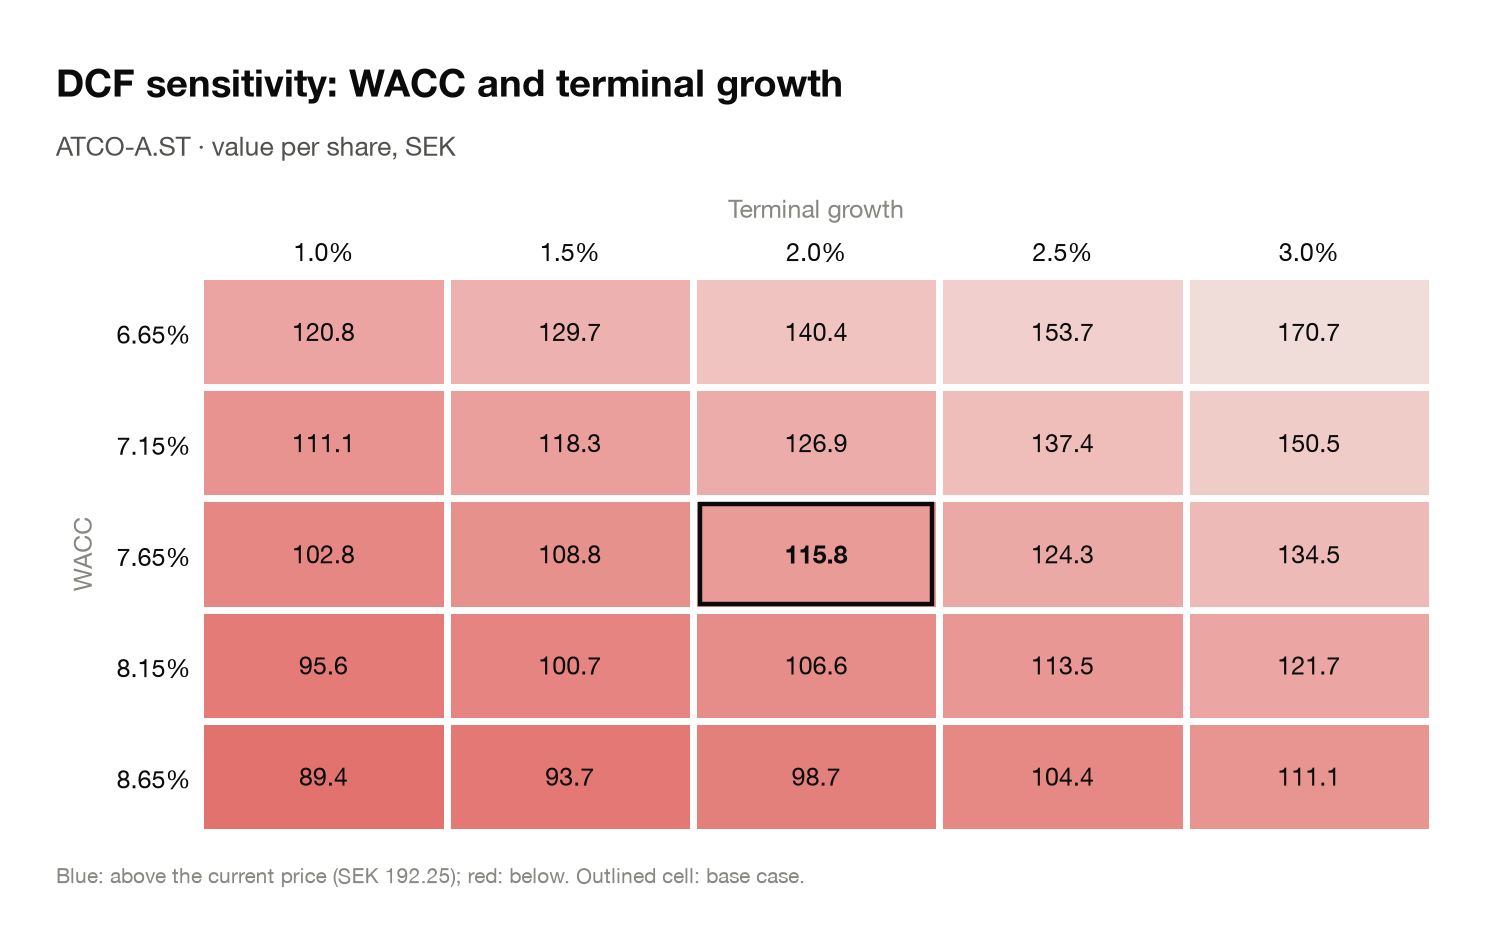
\includegraphics[width=0.8\linewidth]{dcf_sensitivity_wacc_growth.png}
\caption{Värde per aktie för Atlas Copco som funktion av WACC och evig tillväxt. Mittenrutan
är basfallet 115,8\kr.}
\label{fig:dcf-sens}
\end{figure}

\subsection{Vanliga misstag, och motorns egna förenklingar}

\begin{vanligtfel}
\begin{itemize}[leftmargin=1.2em]
  \item Att diskontera FCFF med avkastningskravet på eget kapital, eller FCFE med WACC.
  \item Att halvårsjustera slutvärdet från en exit-multipel, eller glömma justeringen på Gordon.
  \item Att använda bokförda värden som vikter i WACC, eller jämförelsebolagens beta utan att
    först rensa bort deras skuldsättning.
  \item Att sätta $g$ över ekonomins långsiktiga nominella tillväxt.
  \item Att glömma minoritetsintressen, leasingskulder eller pensionsskulder i bryggan.
  \item Att inte kontrollera slutvärdets andel och den implicita multipeln.
\end{itemize}
\end{vanligtfel}

Motorn har också egna förenklingar, och de ska du kunna redogöra för. Det finns ingen
stubbperiod: modellen värderar som om år 1 just hade börjat, fast kursen är från november.
Leasing enligt IFRS~16 gör kassaflödena under prognosåren något för höga. Prognosen är mekanisk
och bygger på högst fyra bokslut. Och tillväxten bromsar till 2\pct{} redan år 5, vilket är
snålt mot ett bolag som marknaden ger en kvalitetspremie.

\section{Multipelvärdering}
\label{sec:multiplar}

En multipelvärdering \eng{comparable company analysis, trading comps} frågar inte vad bolaget
borde vara värt utan vad marknaden betalar för liknande bolag just nu. Man tar ett nyckeltal
för jämförelsebolagen \eng{peers}, till exempel rörelsevärde delat med EBITDA, och multiplicerar
med målbolagets EBITDA. Metoden är snabb, lätt att förklara och förankrad i verkliga priser.
Svagheten är densamma: om hela sektorn är felprissatt blir svaret också fel.

\subsection{Varför multiplar fungerar: en multipel är en hoptryckt DCF}

Ta Gordons formel~\eqref{eq:gordon} för ett bolag i jämvikt, $\EV = \FCFF_1/(r-g)$, och skriv
kassaflödet som en andel $\kappa$ av EBITDA, $\FCFF_1 = \kappa \cdot \EBITDA_1$. Talet $\kappa$
är kassakonverteringen \eng{cash conversion}: hur mycket av EBITDA som blir kvar efter skatt,
investeringar och rörelsekapital. Då är
\begin{equation}
  \frac{\EV}{\EBITDA_1} = \frac{\kappa}{r-g} .
  \label{eq:multipel-dcf}
\end{equation}
Multipeln är alltså inget nytt mått utan en DCF med tre antaganden hoptryckta till ett tal:
kassakonvertering, risk och tillväxt. Två bolag förtjänar samma multipel bara om de är lika i
alla tre. För Atlas Copco ger motorns slutår $\kappa = 0,62$ och $r - g = 5,65$
procentenheter, alltså 11 gånger nästa års EBITDA. Det är samma tal som den implicita
multipeln 11,7 i avsnitt~\ref{sec:gordon}, sånär som på halvårsfaktorn och ett års tillväxt.

Samma härledning för aktiekursen: utdelningen är vinsten gånger utdelningsandelen, och ett
bolag som återinvesterar andelen $g/\mathrm{ROE}$ av vinsten växer med $g$. Alltså
\begin{equation}
  \frac{P}{E_1} = \frac{1 - g/\mathrm{ROE}}{r_e - g} ,
  \label{eq:pe}
\end{equation}
där $P$ är aktiekursen, $E_1$ nästa års vinst per aktie (inte eget kapital, som $E$ betyder i
övrigt) och $\mathrm{ROE}$ avkastningen på eget kapital \eng{return on equity}. Med
$\mathrm{ROE} = 20$\pct, $g = 2$\pct{} och $r_e = 7,84$\pct{} blir P/E
$0,9 / 0,0584 = 15,4$. Jämförelsebolagen i caset handlas till 32,9 gånger vinsten. Marknaden
räknar alltså med högre tillväxt, lägre avkastningskrav eller båda.

\begin{intervjutips}
Frågan ”why would two similar companies trade at different multiples?” besvaras
med~\eqref{eq:multipel-dcf}: olika tillväxt, olika risk eller olika marginal och
kapitalbehov. Säg de tre orden \en{growth}, \en{risk} och \en{returns on capital}.
\end{intervjutips}

\subsection{Vilken multipel till vad}

Grundregeln är att täljare och nämnare ska tillhöra samma finansiärer. Rörelsevärde hör ihop
med mått före räntor (omsättning, EBITDA, EBIT). Börsvärde hör ihop med mått efter räntor
(nettoresultat, eget kapital).

\begin{table}[ht]
\centering\small
\caption{De vanligaste multiplarna. Motorn räknar de tre första.}
\label{tab:multiplar}
\begin{tabularx}{\linewidth}{@{}l>{\raggedright\arraybackslash}X>{\raggedright\arraybackslash}X@{}}
\toprule
Multipel & Använd när & Svaghet \\
\midrule
EV/EBITDA & Standardvalet för mogna rörelsedrivande bolag. Opåverkad av skuldsättning och
  avskrivningsprinciper & Bortser från hur mycket som måste investeras. Meningslös för banker \\
EV/Sales & Bolaget går med förlust eller har tillfälligt pressad marginal & Bortser helt från
  lönsamheten \\
P/E & Banker och andra finansiella bolag. Vanligast bland investerare & Påverkas av
  skuldsättning, skatt och engångsposter \\
EV/EBIT & Bolagen har olika kapitalintensitet & Påverkas av avskrivningsprinciper \\
P/B (kurs mot eget kapital) & Banker och fastighetsbolag & Säger lite om bolag med få bokförda
  tillgångar. Finns inte i motorn \\
\bottomrule
\end{tabularx}
\end{table}

\begin{vanligtfel}
Att blanda nivåerna, till exempel EV delat med nettoresultat eller börsvärde delat med EBITDA.
Lika vanligt: att jämföra multiplar som bygger på olika perioder. Motorn använder senaste
räkenskapsår för alla bolag. På en bank används oftare rullande tolv månader \eng{last twelve
months, LTM} eller nästa års prognos \eng{forward multiple}.
\end{vanligtfel}

\subsection{Klustringens matematik}

På en bank väljs jämförelsebolagen för hand av någon som kan branschen. Motorn måste klara 687
bolag utan hjälp och använder därför klustring. Tre begrepp behövs.

\paragraph{Standardisering.} Bolagen beskrivs med sex variabler: logaritmen av börsvärdet,
omsättningstillväxt, EBITDA-marginal, avkastning på eget kapital, beta och skuldsättning
($D/(D+E)$). De har helt olika skalor, och ett avstånd i rådata hade dominerats av den
variabel som råkar ha störst tal. Varje variabel $j$ räknas därför om till z-värden:
\begin{equation}
  z_{ij} = \frac{x_{ij} - \bar x_j}{s_j},
  \label{eq:z}
\end{equation}
där $\bar x_j$ och $s_j$ är medelvärde och standardavvikelse bland kandidaterna. Före
standardiseringen kapar motorn extremvärden vid 5:e och 95:e percentilen (winsorisering) och
ersätter saknade värden med medianen.

\paragraph{K-means.} Algoritmen delar punkterna $z_1, \dots, z_n$ i $k$ grupper
$C_1, \dots, C_k$ så att summan av kvadrerade avstånd till gruppens medelpunkt $\mu_j$ blir så
liten som möjligt:
\begin{equation}
  J(C_1, \dots, C_k) = \sum_{j=1}^{k} \sum_{i \in C_j} \lVert z_i - \mu_j \rVert^2,
  \qquad \mu_j = \frac{1}{|C_j|} \sum_{i \in C_j} z_i .
  \label{eq:kmeans}
\end{equation}
Att hitta det globala minimumet är NP-svårt. Lloyds algoritm hittar ett lokalt minimum genom
att växla mellan två steg:

\begin{enumerate}
  \item \textbf{Tilldela.} Varje punkt går till närmaste medelpunkt.
  \item \textbf{Uppdatera.} Varje medelpunkt flyttas till medelvärdet av sina punkter.
\end{enumerate}

Inget av stegen kan öka $J$: det första minskar varje punkts term för sig, det andra använder
att medelvärdet är den punkt som minimerar summan av kvadrerade avstånd. Eftersom $J$ är
avtagande och antalet uppdelningar är ändligt stannar algoritmen efter ändligt många steg. Men
resultatet beror på startpunkterna, så motorn kör tio starter med fast slumpfrö
(\kod{n_init=10}, \kod{random_state=42}) och behåller den bästa.

\paragraph{Silhuettvärdet} avgör hur många kluster som passar. För punkt $i$ är $a(i)$
medelavståndet till de andra punkterna i samma kluster och $b(i)$ medelavståndet till punkterna
i närmaste \emph{andra} kluster:
\begin{equation}
  s(i) = \frac{b(i) - a(i)}{\max\{a(i),\, b(i)\}} \in [-1, 1] .
  \label{eq:silhuett}
\end{equation}
Nära 1 betyder att punkten ligger tätt bland de sina och långt från andra. Nära 0 betyder att
den ligger på gränsen. Motorn prövar $k = 2, \dots, 8$ och väljer det $k$ som ger högst
medelvärde av $s(i)$.

\subsection{Hur motorn faktiskt väljer jämförelsebolag}
\label{sec:peers-arligt}

Projektet beskrivs som ”comps med k-means”. Det är sant, men klustringen gör mindre av jobbet
än namnet antyder. Så här går det till för Atlas Copco:

\begin{enumerate}
  \item \textbf{Kandidater.} Bara bolag i samma sektor enligt Yahoo (Industrials) kommer i
    fråga: 148 stycken. Utan den spärren hade klustringen kunnat para ihop en bank med ett
    bioteknikbolag av samma storlek.
  \item \textbf{Klustring.} Silhuettvärdet är högst för $k = 2$ (figur~\ref{fig:silhuett}).
    Av de 148 kandidaterna hamnar 119 i samma kluster som Atlas Copco. Klustringen sorterar
    alltså bort en femtedel och inte mer. I projektets körning över hela universumet väljs $k = 2$ för ungefär
    halva universumet.
  \item \textbf{Rangordning.} Det verkliga urvalet görs av en rangordning efter avstånd i
    z-rummet, med ett straff för annan bransch:
    $\lVert z_i - z_{\text{mål}} \rVert + 0,5 \cdot p_i$, där $p_i = 0$ för samma bransch,
    $0,5$ för samma branschfamilj, $1$ för annan bransch i sektorn och $2$ för annan sektor.
    De tolv närmaste behålls.
  \item \textbf{Rensning.} Multiplar utanför ett Tukey-staket ($1,5$ kvartilavstånd på
    logaritmen av multipeln) tas bort. Här faller ett bolag bort, Electrolux Professional, och
    elva blir kvar.
  \item \textbf{Värde.} Gruppens 25:e percentil, median och 75:e percentil multipliceras med
    målbolagets eget mått och förs genom bryggan~\eqref{eq:brygga}.
\end{enumerate}

\begin{figure}[ht]
\centering
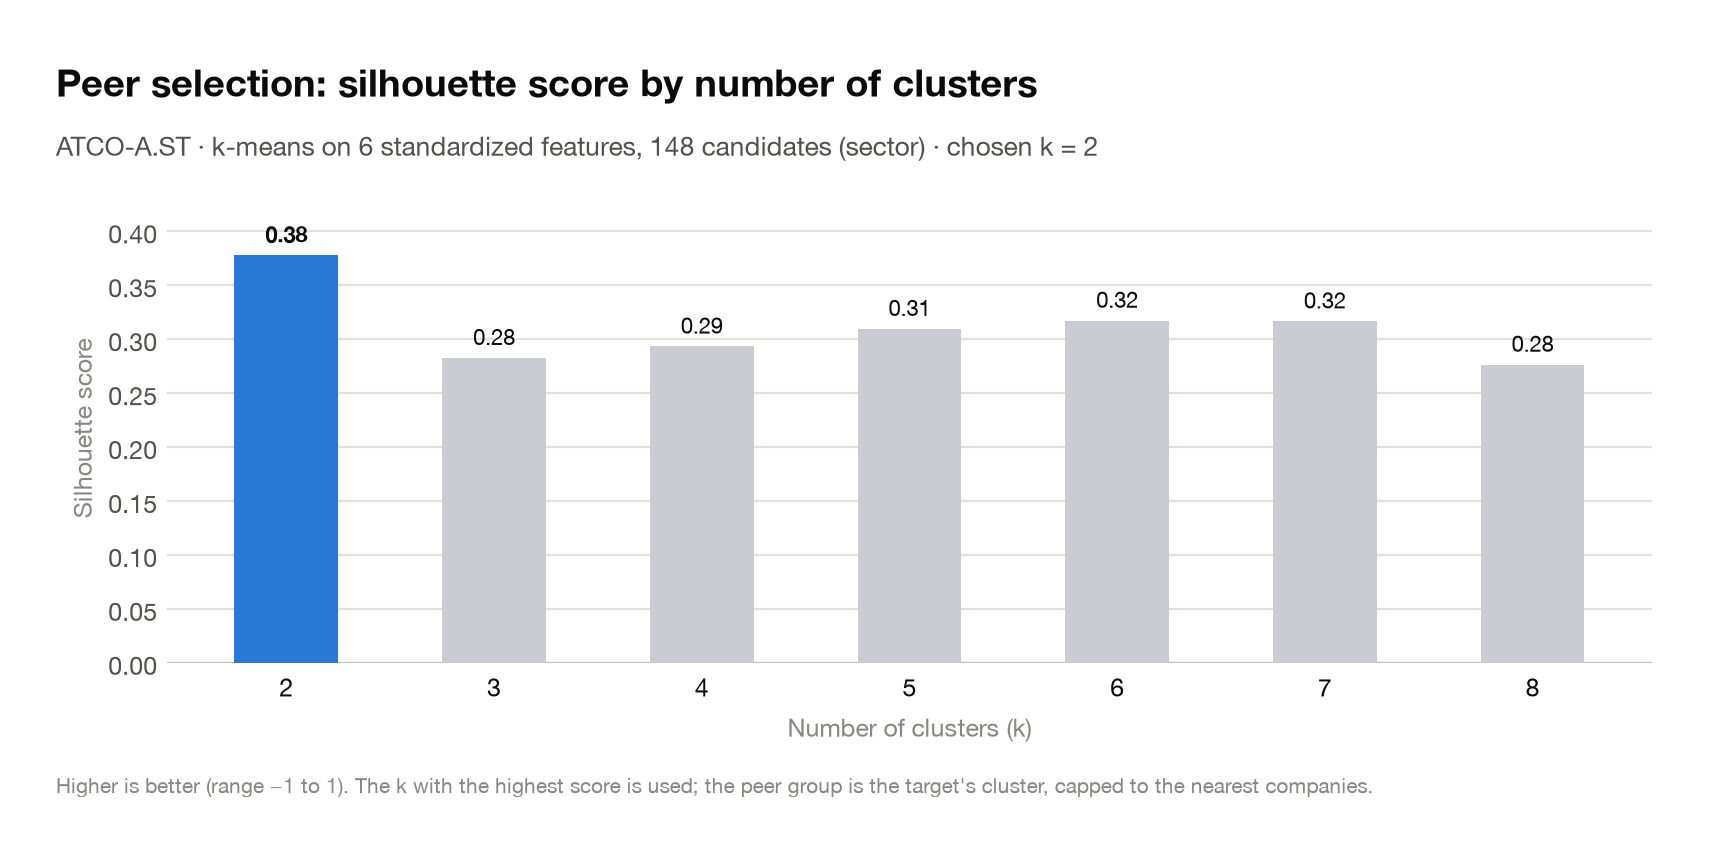
\includegraphics[width=0.72\linewidth]{comps_silhouette.png}
\caption{Silhuettvärde per antal kluster för Atlas Copcos sektor. $k = 2$ vinner, men inget
värde är högt: det finns ingen tydlig klusterstruktur i data.}
\label{fig:silhuett}
\end{figure}

\begin{komihag}
Ärligt beskrivet väljer motorn jämförelsebolag med \emph{närmaste grannar inom sektorn, med
förtur för samma bransch}. K-means bidrar med en grov första sållning. Säg det så i en
intervju. Det är mer trovärdigt än att påstå att en klustringsalgoritm har hittat de rätta
bolagen.
\end{komihag}

Resultatet för Atlas Copco är en blandad grupp: Sandvik, Alfa Laval, Epiroc, Trelleborg,
Mycronic, Lifco, Addtech, Indutrade, Latour, Beijer Alma och Assa Abloy. Alla är mindre än
Atlas Copco, och ett av dem är ett investmentbolag. Figur~\ref{fig:comps} visar deras multiplar.
Räkningen för EV/EBITDA: medianen 19,4 gånger Atlas Copcos EBITDA 44,1~mdkr ger ett
rörelsevärde på 856,6~mdkr. Minus nettoskuld och minoritet (12,6) blir aktievärdet 844,0~mdkr,
eller 172,9\kr{} per aktie.

\begin{figure}[ht]
\centering
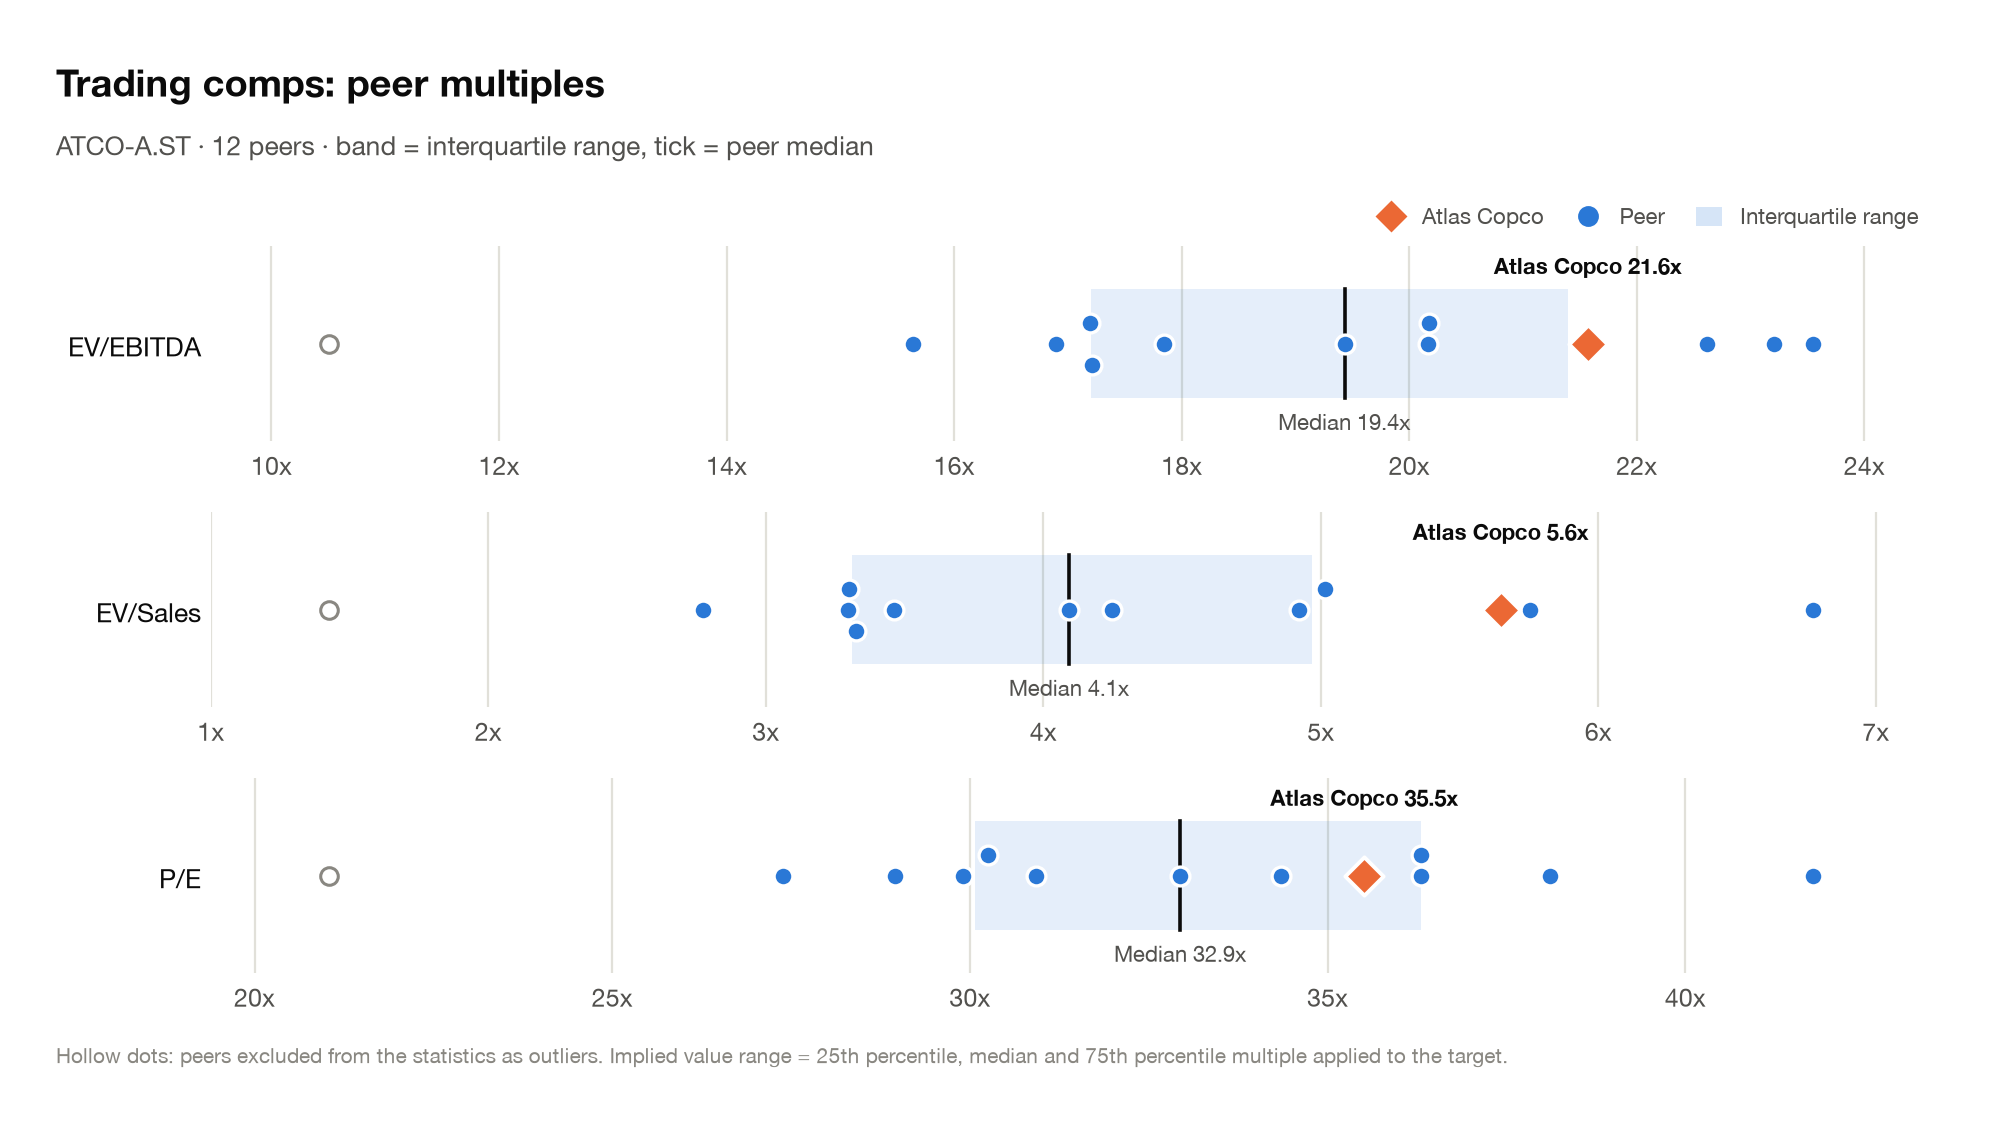
\includegraphics[width=\linewidth]{comps_peer_multiples.png}
\caption{Jämförelsebolagens multiplar. Bandet är kvartilavståndet, strecket medianen och
romben Atlas Copco, som ligger ungefär vid gruppens 75:e percentil på EV/EBITDA och P/E. Den
ofyllda punkten är bolaget som rensades bort.}
\label{fig:comps}
\end{figure}

För banker, försäkringsbolag, investmentbolag och fastighetsbolag räknar motorn bara P/E,
eftersom rörelsevärde och EBITDA inte är meningsfulla när skulden är själva råvaran.
Kandidaterna hämtas då i första hand ur samma branschfamilj (till exempel alla banker), och
klustringen använder bara storlek, avkastning på eget kapital och beta.

\section{LBO: lånefinansierade uppköp}
\label{sec:lbo}

\subsection{Hur en riskkapitalaffär fungerar}

Ett riskkapitalbolag \eng{private equity firm, financial sponsor} köper ett helt bolag, äger
det i några år och säljer det igen. Det speciella är finansieringen: en stor del av köpeskillingen
lånas, och lånen läggs på det köpta bolaget, som betalar ränta och amorteringar ur sitt eget
kassaflöde. Därav namnet \en{leveraged buyout}, LBO.

Varför låna? Ett räkneexempel. Ett bolag med EBITDA 100 köps för 1\,000 (10 gånger EBITDA),
med 600 i lån och 400 i eget kapital. Under fem år ger rörelsen 350 i kassaflöde före räntor.
Av det går 150 till ränta och 200 till amortering. EBITDA växer till 130, och bolaget säljs
till samma multipel, alltså för 1\,300. Skulden är då 400, och ägaren får $1\,300 - 400 = 900$.
Insatsen har vuxit 2,25 gånger, vilket är 17,6\pct{} om året. Utan lån hade ägaren satsat
1\,000 och fått $1\,300 + 350 = 1\,650$: 1,65 gånger pengarna, eller 10,5\pct{} om året. Samma
bolag, samma rörelse, men hävstången lyfter avkastningen på det egna kapitalet. Priset är
risken: om EBITDA faller i stället är det ägarens 400 som försvinner först.

\subsection{Källor och användning}

Varje affär börjar med en uppställning av var pengarna kommer ifrån och vad de används till
\eng{sources and uses}. De två sidorna ska vara lika, och ägarens insats är den post som får
det att gå ihop. Tabell~\ref{tab:sau} är motorns uppställning för Atlas Copco vid kurs plus
30\pct{} budpremie, alltså 249,93\kr{} per aktie.

\begin{table}[H]
\centering\small
\caption{Källor och användning för ett tänkt uppköp av Atlas Copco (mdkr).}
\label{tab:sau}
\begin{tabular}{@{}lrr@{\hspace{2.2em}}lrr@{}}
\toprule
Källor & mdkr & Andel & Användning & mdkr & Andel \\
\midrule
Seniort lån ($4,0 \times$ EBITDA) & 176,3 & 13,7\pct & Köp av aktierna & 1\,219,7 & 94,5\pct \\
Efterställt lån ($1,5 \times$) & 66,1 & 5,1\pct & Lösen av befintlig skuld & 37,5 & 2,9\pct \\
Bolagets egen kassa & 25,1 & 1,9\pct & Transaktionskostnader (2\pct{} av EV) & 24,6 & 1,9\pct \\
Ägarens insats & 1\,022,6 & 79,3\pct & Lånekostnader (2\pct{} av lånen) & 4,8 & 0,4\pct \\
 & & & Kassa som lämnas kvar & 3,4 & 0,3\pct \\
\midrule
Summa & 1\,290,1 & 100\pct & Summa & 1\,290,1 & 100\pct \\
\bottomrule
\end{tabular}
\end{table}

Redan här syns att affären är orealistisk: ägaren skulle behöva över 1\,000~mdkr, och priset
motsvarar 28,0 gånger EBITDA. Exemplet duger ändå för att visa mekaniken.

\subsection{Skuldtrancher}

Skulden delas i skikt \eng{tranches} med olika förmånsrätt, och ju längre bak i kön desto högre
ränta. Motorn har tre:

\begin{description}
  \item[Seniort lån] \eng{senior term loan}: 4,0 gånger EBITDA, ränta riskfri ränta plus 4
    procentenheter (7,075\pct), amorteras med 5\pct{} av ursprungsbeloppet per år och får
    dessutom all överskottskassa.
  \item[Efterställt lån] \eng{subordinated debt, mezzanine}: 1,5 gånger EBITDA, riskfri ränta
    plus 8 procentenheter (11,075\pct), betalas i sin helhet vid förfall \eng{bullet} och
    amorteras aldrig i förtid.
  \item[Checkkredit] \eng{revolving credit facility}: 0,5 gånger EBITDA, outnyttjad vid köpet,
    används bara om kassan inte räcker till ränta och amortering.
\end{description}

Lånen krymps vid behov så att tre villkor håller: EBITDA ska vara minst 2,0 gånger första
årets ränta, EBITDA minus capex minst 1,25 gånger ränta plus amortering, och ägarens insats
minst 30\pct{} av det nya kapitalet. Det efterställda lånet skärs först. Nivåerna (5,5 gånger
EBITDA, räntemarginalerna, 30\pct{} budpremie) är vanliga tumregler i läroböcker, inte
källbelagda marknadsdata.

\subsection{Kassaflödet och svepet}

Varje år går kassan genom en bestämd ordning, ett vattenfall. Överst står det kassaflöde som
finns att betala långivarna med: EBITDA minus skatt, capex och ökat rörelsekapital. Sedan
betalas ränta och obligatorisk amortering. Det som blir över, utöver en minsta kassa på 2\pct{}
av omsättningen, betalar först tillbaka checkkrediten och går sedan till extra amortering av
det seniora lånet. Det sista steget kallas \en{cash sweep}.

\begin{lstlisting}[caption={Vattenfallet i \texttt{\_project}, \texttt{models/lbo.py}
(förkortat).},label=lst:sweep]
cfads = ebitda - tax - capex - change_in_nwc
cash_interest = total_interest - sub_pik
mandatory = min(scheduled, senior)
excess_cash_flow = cfads - cash_interest - mandatory
surplus = cash + excess_cash_flow - minimum_cash
revolver_draw = min(max(-surplus, 0.0), max(revolver_limit - revolver, 0.0))
revolver_repayment = min(max(surplus, 0.0), revolver)
sweep = min(
    a.cash_sweep_pct * max(surplus - revolver_repayment, 0.0),
    senior - mandatory,
)
\end{lstlisting}

Två detaljer är värda att känna till. Räntan räknas på årets \emph{ingående} skuld, vilket gör
att modellen slipper cirkelreferensen mellan ränta och amortering som Excel-modeller brukar ha.
Och skatten räknas på EBIT minus avdragsgill ränta, där avdraget begränsas till 30\pct{} av
EBITDA, en förenkling av de svenska reglerna om ränteavdragsbegränsning. För Atlas Copco är
räntan första året 19,8~mdkr, men bara 14,1 får dras av.

\begin{figure}[ht]
\centering
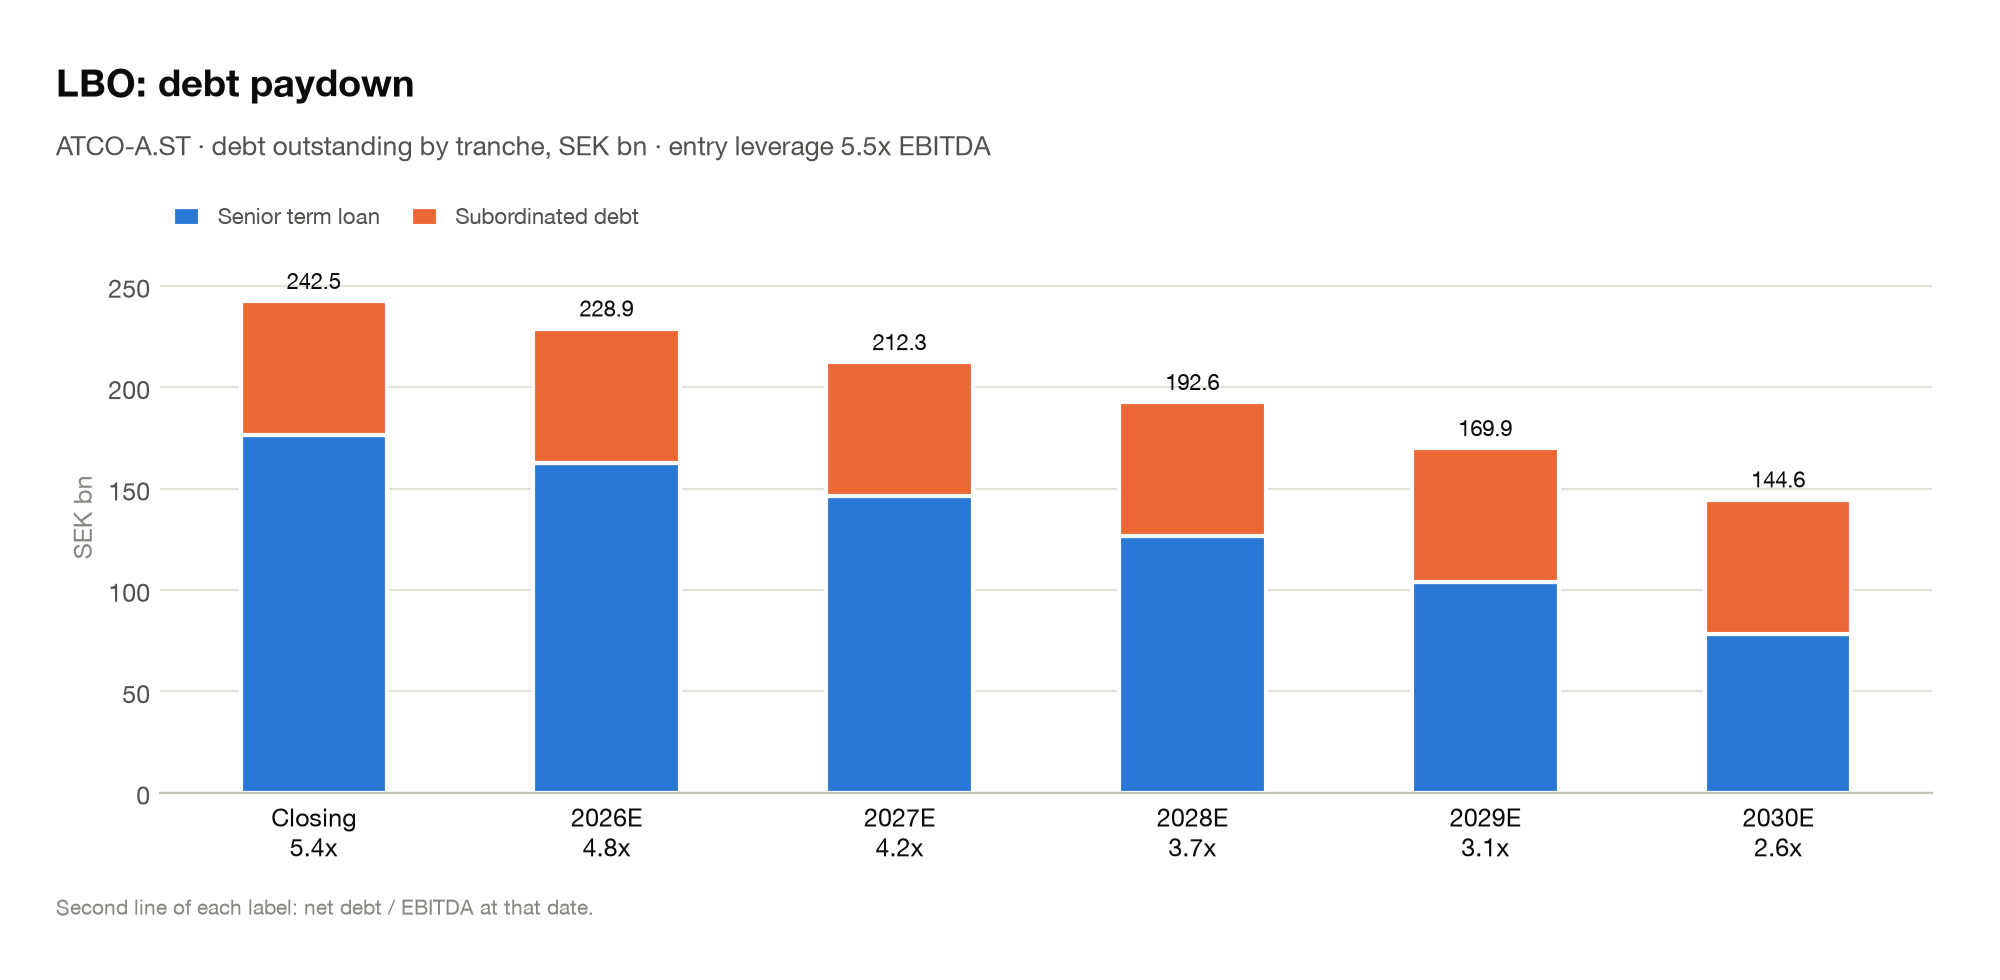
\includegraphics[width=0.92\linewidth]{lbo_debt_paydown.png}
\caption{Skulden år för år i motorns LBO på Atlas Copco. Det seniora lånet amorteras från 176
till 78~mdkr, det efterställda ligger kvar på 66.}
\label{fig:lbo-skuld}
\end{figure}

\subsection{Varifrån avkastningen kommer}
\label{sec:lbo-attribution}

Ägarens insats är köpets rörelsevärde plus avgifter minus nettoskulden efter köpet. Det ägaren
får vid försäljningen är rörelsevärdet då minus nettoskulden då. Skriv rörelsevärdet som
multipel gånger EBITDA, med index 0 för köpet och $x$ för försäljningen. Skillnaden blir
\begin{equation}
  {\underbrace{E_x - E_0}_{\text{värdeskapande}}}
  = {\underbrace{(\EBITDA_x - \EBITDA_0)\, M_0}_{\text{resultattillväxt}}}
  + {\underbrace{(M_x - M_0)\, \EBITDA_x}_{\text{multipelförändring}}}
  + {\underbrace{(\mathrm{ND}_0 - \mathrm{ND}_x)}_{\text{amortering}}}
  - \text{avgifter}.
  \label{eq:attribution}
\end{equation}
Identiteten följer av att
$M_x \EBITDA_x - M_0 \EBITDA_0 = (\EBITDA_x - \EBITDA_0) M_0 + (M_x - M_0)\EBITDA_x$. Det är de
tre källorna till avkastning som varje intervjuare vill höra: bolaget tjänar mer \eng{EBITDA
growth}, det säljs dyrare än det köptes \eng{multiple expansion}, och skulden har betalats
ned med bolagets egna pengar \eng{debt paydown, deleveraging}.

För Atlas Copco, köpt till 28,0 och sålt till 19,4 gånger EBITDA (figur~\ref{fig:lbo-vf}):
$278,5 - 460,7 + 98,6 - 29,5 = -113,1$~mdkr. Ägaren får tillbaka 909 av 1\,023~mdkr.
Resultattillväxt och amortering räcker inte när multipeln faller så mycket.

\begin{figure}[ht]
\centering
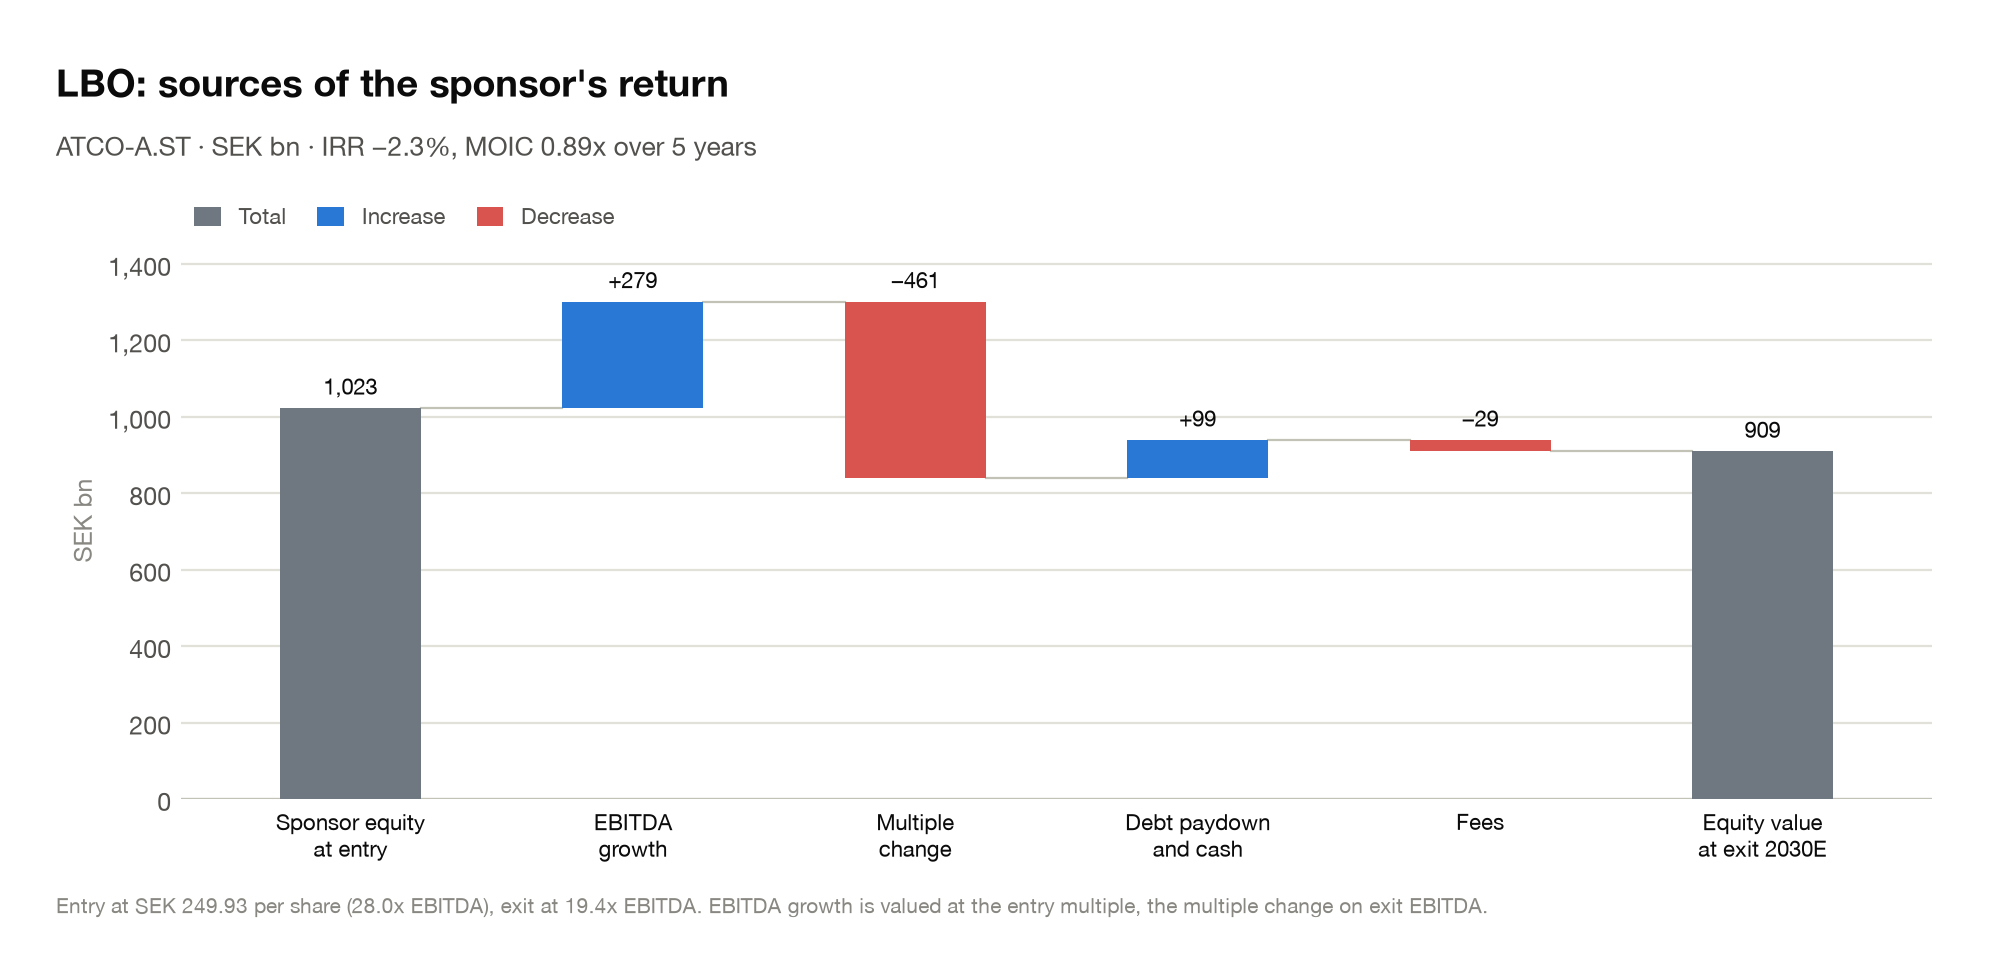
\includegraphics[width=0.92\linewidth]{lbo_returns_waterfall.png}
\caption{Uppdelningen~\eqref{eq:attribution} för Atlas Copco vid kurs plus 30\pct{} premie.}
\label{fig:lbo-vf}
\end{figure}

\subsection{IRR och MOIC}

Två mått används. MOIC \eng{multiple on invested capital} är pengar ut delat med pengar in.
IRR, internräntan \eng{internal rate of return}, är den ränta som gör nuvärdet av ägarens
alla kassaflöden $C_0, \dots, C_N$ till noll:
\begin{equation}
  \sum_{t=0}^{N} \frac{C_t}{(1+\IRR)^t} = 0 .
  \label{eq:irr}
\end{equation}

\paragraph{IRR som rot till ett polynom.} Sätt $x = 1/(1+\IRR)$. Då är~\eqref{eq:irr} ekvationen
$p(x) = \sum_t C_t x^t = 0$, ett polynom av grad $N$, och vi söker rötter med $x > 0$. Tre
saker är värda att kunna:

\begin{itemize}
  \item \textbf{Existens och entydighet.} Om kassaflödena byter tecken exakt en gång (först en
    insats, sedan bara inflöden) har $p$ enligt Descartes teckenregel exakt en positiv rot. Då
    finns precis en internränta över $-100$\pct.
  \item \textbf{Flera rötter.} Med flera teckenbyten kan det finnas flera. Flödena
    $-100, +230, -132$ ger $100(1+r)^2 - 230(1+r) + 132 = 0$ med rötterna $r = 10$\pct{} och
    $r = 20$\pct. Motorns \kod{compute_irr} returnerar då den minsta.
  \item \textbf{Varför rotsökning.} För grad fem och högre finns ingen allmän lösningsformel
    (Abel och Ruffini), så internräntan måste sökas numeriskt. Motorn använder Brents metod
    (\kod{scipy.optimize.brentq}), som kombinerar intervallhalvering med interpolation och
    alltid konvergerar när funktionen byter tecken på intervallet.
\end{itemize}

I motorns LBO finns inga utdelningar under innehavet, så ägarens flöden är bara insatsen och
försäljningen. Då har~\eqref{eq:irr} en sluten lösning:
\begin{equation}
  \IRR = \MOIC^{1/N} - 1 .
  \label{eq:irr-moic}
\end{equation}
För Atlas Copco: $\MOIC = 909/1\,023 = 0,89$ och $\IRR = 0,89^{1/5} - 1 = -2,3$\pct{} om året.

\begin{komihag}
MOIC säger hur mycket, IRR säger hur fort. Dubbla pengarna på tre år är 26\pct{} om året, på
fem år 15\pct. Tre gånger pengarna på fem år är 25\pct. En fond som säljer tidigt kan visa hög
IRR med låg MOIC, och därför tittar investerare på båda.
\end{komihag}

\subsection{Betalningsförmåga: LBO som värderingsmetod}

Till football field behövs ett pris, inte en avkastning. Motorn vänder därför på frågan: vilket
pris per aktie $P$ kan en riskkapitalköpare betala och ändå nå sitt avkastningskrav? Det kallas
\en{ability to pay}. Motorn söker roten till
\begin{equation}
  f(P) = -E_0(P) + \frac{E_x(P)}{(1 + \IRR^{*})^N} = 0,
  \label{eq:atp}
\end{equation}
där $E_0(P)$ är insatsen och $E_x(P)$ försäljningslikviden vid priset $P$. Här behövs
rotsökningen på riktigt, eftersom lånevillkoren gör $E_0$ och $E_x$ till styckvis definierade
funktioner av $P$. Stapelns ändar är tre avkastningskrav: 25\pct{} ger det låga priset,
20\pct{} basvärdet och 15\pct{} det höga. Kraven är vanliga tumregler för vad riskkapitalfonder
siktar på.

För Atlas Copco blir priserna 104,4, 117,9 och 135,3\kr. Vid 117,9\kr{} motsvarar köpet 13,3
gånger EBITDA, insatsen är 60\pct{} av det nya kapitalet och pengarna växer 2,49 gånger på fem
år, vilket är exakt 20\pct{} om året. Lånen är desamma som i tabell~\ref{tab:sau}, eftersom de
bestäms av EBITDA och inte av priset. Lägre pris betyder därför mindre eget kapital och högre
hävstång.

\begin{intervjutips}
En LBO-värdering kallas ofta ett golv \eng{floor valuation}: en finansiell köpare har inga
synergier och ett högt avkastningskrav, så en industriell köpare bör kunna betala mer. Lägg
märke till att LBO-värdet i caset (118\kr) hamnar nära Gordon-DCF:en (116\kr). Det är samma
kassaflöden, värderade med 20\pct{} avkastningskrav och lånefinansiering till hjälp i stället
för 7,65\pct{} utan.
\end{intervjutips}

\section{Monte Carlo-simulering}
\label{sec:mc}

\subsection{Varför simulera?}

En DCF ger ett tal, men talet är en funktion av antaganden som ingen känner. En
känslighetstabell varierar två av dem i taget. En Monte Carlo-simulering varierar alla på en
gång: man drar antagandena ur sannolikhetsfördelningar, räknar DCF:en en gång per dragning och
får en fördelning av värden i stället för ett tal. Här har du som matematiker ett försprång.
Det mesta är sannolikhetslära du redan kan, och det svåra är att vara ärlig med vad resultatet
betyder.

Motorn simulerar fyra drivare som \emph{förskjutningar} från basfallet: omsättningstillväxt och
EBITDA-marginal (samma förskjutning alla prognosår), WACC och evig tillväxt. Allt annat ligger
fast. Varje dragning värderas med samma funktion \kod{dcf_core} som basfallet, i ett enda
vektoriserat anrop utan slinga över simuleringarna.

\subsection{Val av fördelningar}

\begin{description}
  \item[Normalfördelning.] Naturlig för summan av många små störningar, men obegränsad. Det är
    ett problem här: en dragning med $\WACC \le g$ får Gordons formel att explodera.
  \item[Trunkerad normalfördelning.] En normalfördelning avskuren vid $\mu \pm 2\sigma$. Det är
    motorns standardval, eftersom den behåller klockformen men utesluter orimliga värden.
    Avskärningen sänker den faktiska standardavvikelsen till $0,88\sigma$.
  \item[Triangelfördelning.] Bestäms av minsta, troligaste och största värde. Den är lätt att
    fråga en expert om (”vad är det lägsta, troligaste och högsta du kan tänka dig?”) och får
    vara sned. En symmetrisk triangel med standardavvikelse $\sigma$ har halvbredden
    $\sqrt6\,\sigma$.
\end{description}

Alla tre dras med inversmetoden: om $U$ är likformig på $(0, 1)$ och $F$ är en
fördelningsfunktion har $X = F^{-1}(U)$ fördelningen $F$. För den trunkerade
normalfördelningen på $[a, b]$ är
$F^{-1}(u) = \mu + \sigma\,\Phi^{-1}\bigl(\Phi(\alpha) + u\,[\Phi(\beta) - \Phi(\alpha)]\bigr)$
med $\alpha = (a-\mu)/\sigma$ och $\beta = (b-\mu)/\sigma$.

\paragraph{Standardavvikelserna är antaganden.} Motorn sätter dem så här: tillväxt hälften av
den historiska standardavvikelsen i årlig tillväxt, marginal den historiska standardavvikelsen,
båda begränsade till 1 till 5 procentenheter, WACC 1 procentenhet och evig tillväxt 0,5. För
Atlas Copco är den historiska spridningen i tillväxt 14 procentenheter (tre observationer:
$+22$, $+2$ och $-5$\pct), så tillväxten slår i taket på 5. Marginalen har varierat så lite
(0,4 procentenheter) att den hamnar på golvet 1.

\subsection{Korrelerade dragningar: Cholesky och Gaussisk copula}

Drivarna är inte oberoende. Motorn antar att tillväxt och marginal samvarierar med
korrelationen $+0,3$ (ett bolag som växer fortare sprider sina fasta kostnader på fler sålda
enheter). Hur drar man korrelerade tal?

\paragraph{Steg 1: Cholesky.} Låt $z$ vara en vektor av oberoende standardnormala variabler, så
att $\E[z] = 0$ och $\Cov(z) = \E[z z\T] = I$. Låt $\Sigma$ vara den korrelationsmatris vi
vill ha. Eftersom $\Sigma$ är symmetrisk och positivt definit finns en entydig undre
triangulär matris $L$ med positiv diagonal så att $\Sigma = L L\T$
(Choleskyfaktoriseringen). Sätt $x = L z$. Då är
\begin{equation}
  \Cov(x) = \E\bigl[(Lz)(Lz)\T\bigr] = L\, \E[z z\T]\, L\T = L I L\T = \Sigma .
  \label{eq:cholesky}
\end{equation}
En linjär avbildning av en normalfördelad vektor är normalfördelad, så $x \sim N(0, \Sigma)$.
I två dimensioner med korrelation $\rho$:
\begin{equation}
  L = \begin{pmatrix} 1 & 0 \\ \rho & \sqrt{1-\rho^2} \end{pmatrix},
  \qquad x_1 = z_1, \quad x_2 = \rho z_1 + \sqrt{1-\rho^2}\, z_2 .
  \label{eq:cholesky2}
\end{equation}
Kravet på positiv definithet är inte en teknikalitet. En matris med parvisa korrelationer som
inte går ihop (A följer B, B följer C, men A går mot C) har ett negativt egenvärde, och då
finns ingen fördelning med de korrelationerna. Motorn kontrollerar det och ger ett begripligt
fel.

\paragraph{Steg 2: copula.} Cholesky ger korrelerade \emph{normalfördelade} tal, men drivarna
ska ha andra fördelningar. Lösningen är att gå via likformiga tal. Om $x_j \sim N(0, 1)$ är
$u_j = \Phi(x_j)$ likformig på $(0, 1)$, och $F_j^{-1}(u_j)$ har den önskade
marginalfördelningen $F_j$. Sambandet mellan variablerna följer med genom båda stegen, eftersom
båda avbildningarna är växande. Konstruktionen kallas Gaussisk copula: beroendet kommer från
en normalfördelning, marginalerna väljs fritt.

\begin{lstlisting}[caption={Dragningen i \texttt{run\_monte\_carlo} och copula-steget i
\texttt{\_transform}, \texttt{models/monte\_carlo.py}.},label=lst:mc]
rng = np.random.default_rng(config.seed)
cholesky = np.linalg.cholesky(correlation)
normals = rng.standard_normal((n, len(DRIVERS))) @ cholesky.T
offsets = {name: _transform(specs[name], normals[:, i]) for i, name in enumerate(DRIVERS)}

# in _transform: standard normal -> uniform -> marginal distribution
uniform = np.clip(ndtr(normals), _UNIFORM_EPS, 1.0 - _UNIFORM_EPS)
return _quantile(spec, uniform)
\end{lstlisting}

Raden \kod{@ cholesky.T} är~\eqref{eq:cholesky} för alla dragningar på en gång: varje rad i
matrisen är ett $z\T$, och $z\T L\T = (Lz)\T$. En detalj för den noggranne: korrelationen
anges på normalskalan. Rangkorrelationen bevaras exakt av de växande avbildningarna, men den
vanliga (Pearson) korrelationen mellan de färdiga drivarna blir något lägre än $0,3$ när
marginalerna inte är normala.

\subsection{Konvergens}

Medelvärdet av $n$ oberoende dragningar har enligt centrala gränsvärdessatsen medelfelet
\eng{standard error}
\begin{equation}
  \mathrm{SE}(\bar V_n) = \frac{s}{\sqrt{n}},
  \label{eq:se}
\end{equation}
där $s$ är stickprovets standardavvikelse. Felet avtar som $1/\sqrt{n}$: tio gånger bättre
precision kräver hundra gånger fler dragningar. Tabell~\ref{tab:konvergens} visar projektets
egna tal, och de följer regeln väl: mellan 687 och 10\,000 dragningar ökar $n$ med en faktor
14,6 och medelfelet faller med en faktor 3,8, mot väntade $\sqrt{14,6} = 3,8$.

\begin{table}[H]
\centering\small
\caption{Konvergens för Atlas Copco (slumpfrö 42, värde per aktie i kr, $s = 32,7$).}
\label{tab:konvergens}
\begin{tabular}{@{}rrrr@{}}
\toprule
Dragningar $n$ & Löpande medelvärde & Löpande median & Medelfel \\
\midrule
83 & 119,2 & 116,6 & 3,49 \\
687 & 121,6 & 116,6 & 1,24 \\
2\,812 & 121,3 & 116,2 & 0,62 \\
10\,000 & 121,6 & 116,7 & 0,33 \\
\bottomrule
\end{tabular}
\end{table}

Med 10\,000 dragningar är medelfelet 0,33\kr, eller 0,3\pct{} av värdet. Caset bekräftar det:
100\,000 dragningar med ett annat slumpfrö flyttar intervallet mellan 10:e och 90:e
percentilen från 84,3 till 164,9 till 84,0 till 165,2\kr. Simuleringen har alltså konvergerat.

\begin{komihag}
Precisionen i~\eqref{eq:se} gäller \emph{räknandet}, inte antagandena. Fler dragningar gör inte
standardavvikelserna mer rätt. I caset krymper intervallet från 84 till 165 till 90 till 155\kr{}
när tillväxtens standardavvikelse sänks från 5 till 3 procentenheter. Det är en
mångdubbelt större effekt än den av tio gånger fler dragningar.
\end{komihag}

\subsection{Varför medelvärdet ligger över basfallet: Jensens olikhet}

Simuleringen för Atlas Copco ger medianen 116,7\kr, nära basfallets 115,8, men medelvärdet
121,6. Det beror inte på att simuleringen har hittat en uppsida. För en konvex funktion $f$ och
en stokastisk variabel $X$ gäller Jensens olikhet:
\begin{equation}
  \E[f(X)] \ge f(\E[X]) .
  \label{eq:jensen}
\end{equation}
Gordon-värdet beter sig som $f(r) = 1/(r-g)$, som är konvex för $r > g$ eftersom
$f''(r) = 2/(r-g)^3 > 0$. Symmetrisk osäkerhet i $r$ ger därför en sned fördelning av värdet
med lång svans uppåt. Ett räkneexempel: med $g = 2$\pct{} och WACC antingen 6,65 eller
8,65\pct{} med lika sannolikhet blir $f$ antingen 21,5 eller 15,0. Medelvärdet 18,3 ligger
3,2\pct{} över $f(7,65\,\%) = 17,7$. Taylorutveckling till andra ordningen ger samma sak
allmänt: $\E[f(X)] \approx f(\mu) + \tfrac12 f''(\mu)\,\sigma^2$, det vill säga en relativ
höjning med $\sigma^2/(r-g)^2$. Därför redovisar motorn medianen, inte medelvärdet, som
centralt värde i football field.

\begin{figure}[ht]
\centering
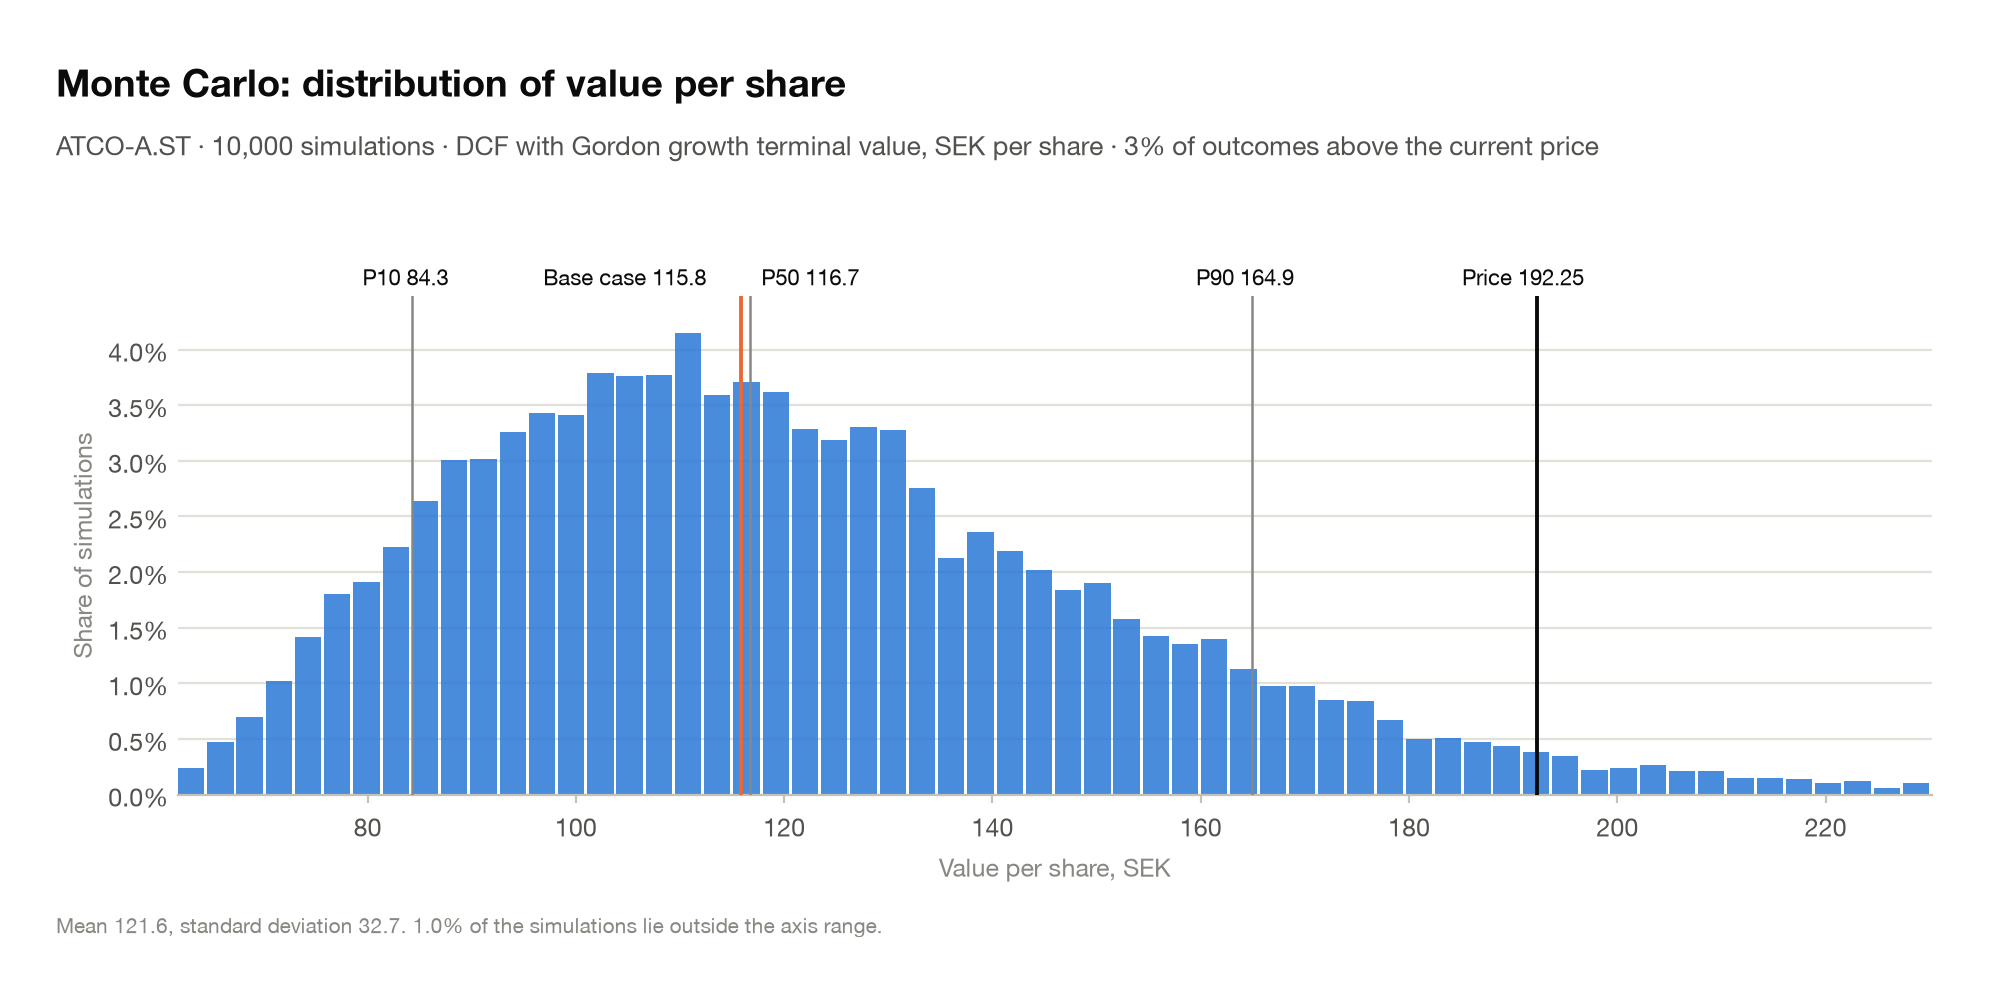
\includegraphics[width=0.95\linewidth]{mc_histogram.png}
\caption{Fördelningen av 10\,000 simulerade DCF-värden för Atlas Copco. Lägg märke till den
långa högersvansen.}
\label{fig:mc-hist}
\end{figure}

\subsection{Tornado och variansbidrag}

Två diagram visar vilka antaganden som betyder mest.

\paragraph{Tornadodiagrammet} (figur~\ref{fig:tornado}) ändrar en drivare i taget till sin 10:e
och 90:e percentil medan de andra ligger kvar i basfallet. För Atlas Copco flyttar tillväxten
värdet mellan 90,7 och 147,1\kr, WACC mellan 96,0 och 146,1, evig tillväxt mellan 107,6 och
126,0 och marginalen mellan 109,2 och 122,5.

\begin{figure}[ht]
\centering
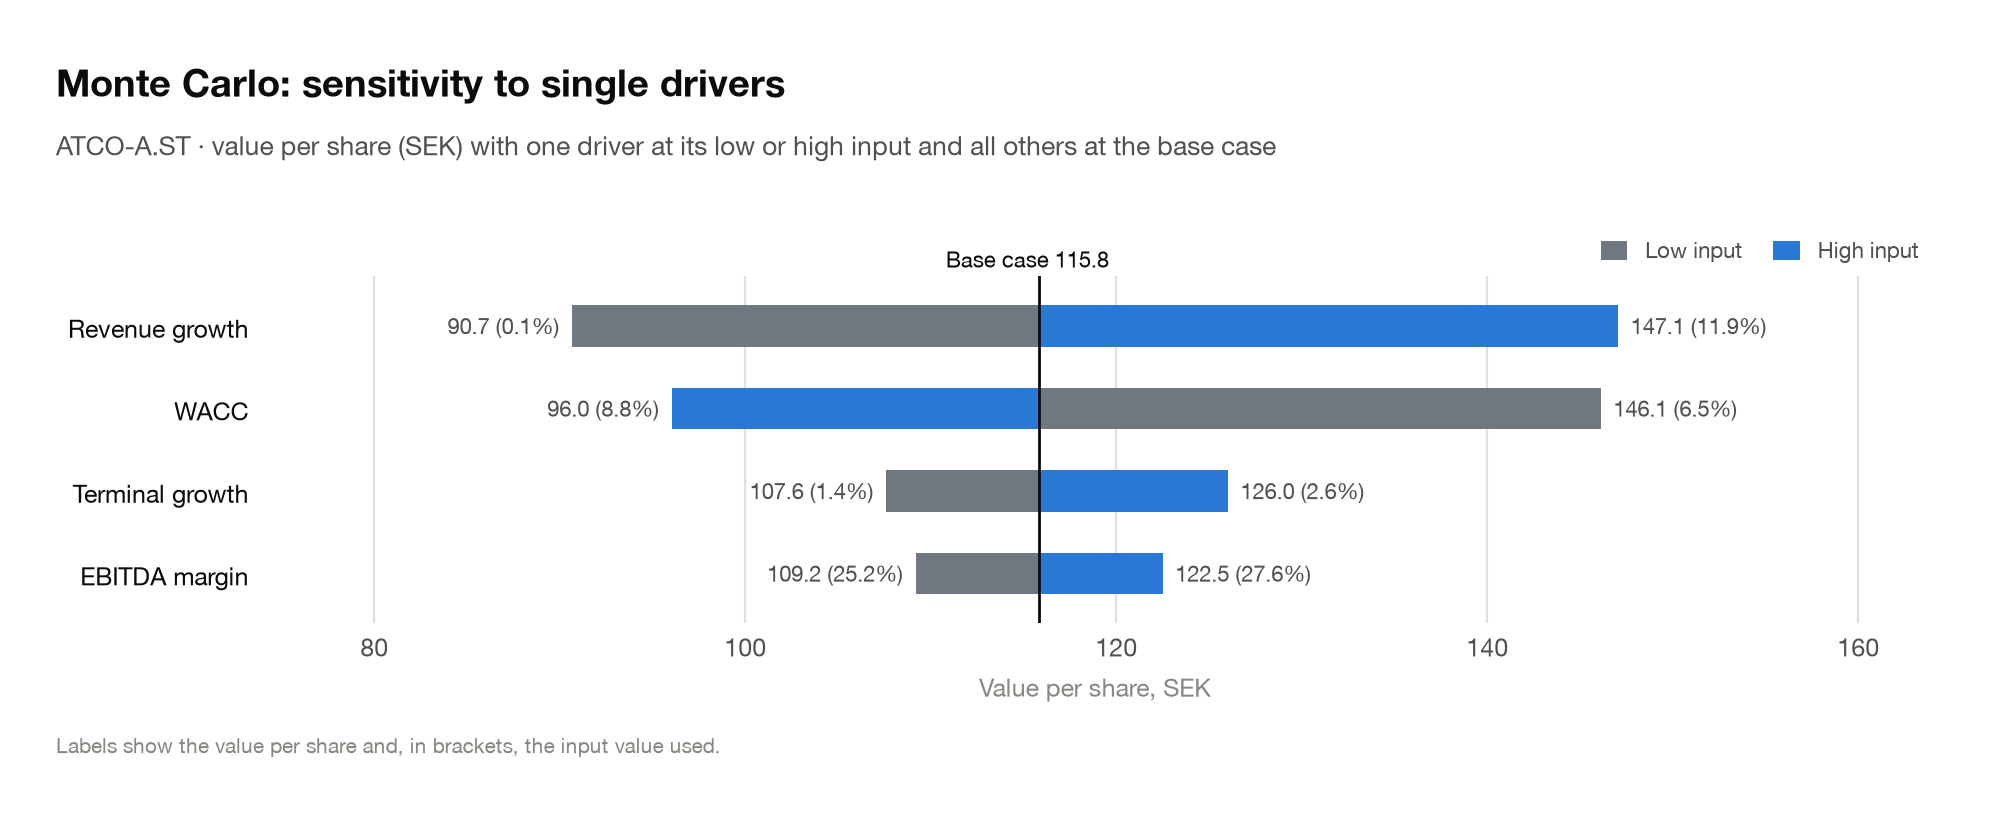
\includegraphics[width=0.95\linewidth]{mc_tornado.png}
\caption{Tornadodiagram: en drivare i taget mellan sin 10:e och 90:e percentil.}
\label{fig:tornado}
\end{figure}

\paragraph{Variansbidraget} mäts i motorn som den kvadrerade rangkorrelationen (Spearman)
mellan varje drivare och det simulerade värdet, normerad så att summan blir 1. För en linjär
modell med oberoende indata är den kvadrerade korrelationen precis drivarens andel av
variansen. Rangkorrelation används för att värdet är monotont men starkt olinjärt i WACC och
$g$. För Atlas Copco: tillväxt 51\pct, WACC 32\pct, marginal 12\pct{} och evig tillväxt 5\pct.

\begin{vanligtfel}
Att läsa in för mycket. (1) Båda diagrammen speglar de standardavvikelser man har matat in:
tillväxten väger tyngst delvis för att dess spridning ligger i taket. (2) Variansbidragen är
en rangordning, ingen riktig variansuppdelning. Med korrelerade indata överlappar de,
samspelseffekter (till exempel mellan WACC och $g$) syns inte, och normeringen döljer hur
mycket som inte förklaras alls. (3) Att 3,3\pct{} av dragningarna ligger över kursen är ingen
sannolikhet för att aktien är undervärderad. Det är ett påstående om modellen givet dess
antaganden.
\end{vanligtfel}

\section{Kodgenomgång}
\label{sec:kod}

\subsection{Arkitektur}

Koden är byggd i lager, och pilarna i figur~\ref{fig:arkitektur} går bara åt ett håll.
Datalagret vet ingenting om modellerna, modellerna vet ingenting om diagram, och allt möts i
ett gemensamt kontrakt: datatyperna i \kod{core/types.py}. Det gör att varje del kan testas för
sig och bytas ut.

\begin{figure}[ht]
\centering
\begin{tikzpicture}[font=\footnotesize\sffamily,
  srcbox/.style={draw=black!45,rounded corners=2pt,fill=black!4,align=center,inner sep=4pt,
              minimum height=9mm,minimum width=4.5cm},
  layerbox/.style={draw=accent,rounded corners=2pt,fill=accent!5,align=center,inner sep=5pt,
              minimum width=15cm,text width=14.4cm},
  modelbox/.style={draw=accent,rounded corners=2pt,fill=white,align=center,inner sep=3pt,
              minimum width=2.75cm,minimum height=11mm},
  outbox/.style={draw=boxgreen,rounded corners=2pt,fill=boxgreen!6,align=center,inner sep=3pt,
              minimum width=3.55cm,minimum height=12mm},
  flow/.style={-{Stealth[length=5pt]},thick,draw=black!60},
  lbl/.style={font=\scriptsize\sffamily,text=black!70,inner sep=1pt}]
  % data layer and its sources
  \node[layerbox] (data) {\textbf{data/}\quad \texttt{yahoo.py},
    \texttt{riksbank.py} $\rightarrow$ \texttt{store.py} (cache och fixtures) $\rightarrow$
    \texttt{mapping.py}, \texttt{fx.py}, \texttt{universe.py} $\rightarrow$ \texttt{loader.py},
    \texttt{market\_params.py}};
  \node[srcbox,above=7mm of data] (riks) {Riksbanken\\ (riskfri ränta, valutakurser)};
  \node[srcbox,anchor=south west] (yahoo) at ($(data.north west)+(0,7mm)$)
    {Yahoo Finance\\ (bokslut, kurser, universum)};
  \node[srcbox,anchor=south east] (damo) at ($(data.north east)+(0,7mm)$)
    {Referensfil, Damodaran\\ (riskpremie, skattesats)};
  \node[layerbox,below=6mm of data,fill=white] (types) {\textbf{core/types.py}\quad
    \texttt{CompanyData}\enspace \texttt{PeerSnapshot}\enspace \texttt{MarketParameters}\enspace
    \texttt{DCFAssumptions}\enspace \texttt{ValuationResult}};
  % models inside the pipeline
  \node[modelbox,anchor=north west] (comps) at ($(types.south west)+(2.5mm,-14mm)$)
    {\textbf{comps.py}\\ jämförelsebolag};
  \node[modelbox,right=12.5mm of comps] (dcf) {\textbf{dcf.py}\\ WACC och DCF};
  \node[modelbox,right=12.5mm of dcf] (lbo) {\textbf{lbo.py}\\ LBO};
  \node[modelbox,right=12.5mm of lbo] (mc) {\textbf{monte\_carlo.py}\\ simulering};
  \coordinate (padtop) at ($(comps.north west)+(0,1.5mm)$);
  \coordinate (padbottom) at ($(mc.south east)+(0,-6mm)$);
  \node[draw=accent,dashed,rounded corners=3pt,inner xsep=2.5mm,inner ysep=2mm,
        fit=(padtop)(padbottom)(comps)(mc)] (pipe) {};
  \node[font=\footnotesize\sffamily\bfseries,text=accent,fill=white,inner sep=2pt,anchor=west]
        at ($(pipe.north west)+(3mm,0)$) {pipeline.py kör modellerna i models/};
  \node[layerbox,below=7mm of pipe,fill=white,minimum width=6cm,text width=5.6cm] (report)
    {\textbf{ValuationReport}\quad alla resultat för ett bolag};
  % outputs
  \node[outbox,anchor=north west] (viz) at ($(report.south -| types.west)+(0,-9mm)$)
    {\textbf{viz/}\\ 16 diagram, football field};
  \node[outbox,right=2.67mm of viz] (xl) {\textbf{export/excel.py}\\ arbetsbok, sju flikar};
  \node[outbox,right=2.67mm of xl] (app) {\textbf{app/streamlit\_app.py}\\ webbapp};
  \node[outbox,right=2.67mm of app] (cli) {\textbf{\_\_main\_\_.py}, \textbf{batch.py}\\
    kommandorad, alla bolag};
  % edges
  \draw[flow] (yahoo.south) to (yahoo.south |- data.north);
  \draw[flow] (riks.south) to (data.north);
  \draw[flow] (damo.south) to (damo.south |- data.north);
  \draw[flow] (data.south) to (types.south |- data.south) to (types.north);
  \draw[flow] (types.south) to (types.south |- pipe.north);
  \draw[flow] (comps.east) to node[lbl,above=1pt] {peers} (dcf.west);
  \draw[flow] (dcf.east) to node[lbl,above=1pt] {prognos} (lbo.west);
  \draw[flow] (dcf.south) to[out=-18,in=-162,looseness=0.45]
    node[lbl,below=0.5pt,pos=0.5] {basfall} (mc.south);
  \draw[flow] (pipe.south) to (report.north);
  \coordinate (bus) at ($(report.south)+(0,-4.5mm)$);
  \draw[thick,draw=black!60] (report.south) to (bus);
  \draw[flow] (bus) -| (viz.north);
  \draw[flow] (bus) -| (xl.north);
  \draw[flow] (bus) -| (app.north);
  \draw[flow] (bus) -| (cli.north);
\end{tikzpicture}
\caption{Arkitekturen: data, modeller, pipeline och presentation. Pipelinen kör comps först och
skickar jämförelsebolagen till DCF:en. LBO:n får DCF:ens prognos och exit-multipel, och
simuleringen utgår från DCF:ens basfall.}
\label{fig:arkitektur}
\end{figure}

\subsection{Modul för modul}

\begin{description}
  \item[\kod{core/types.py}] Kontraktet. Alla belopp är absoluta tal i bolagets handelsvaluta,
    kostnader lagras som positiva tal, och räntor som decimaltal. En post som saknas är
    \kod{NaN}, aldrig en saknad kolumn. Tabell~\ref{tab:typer} listar de viktigaste typerna.
  \item[\kod{data/}] \kod{yahoo.py} är den enda modul som pratar med nätet. Den sparar råa svar
    som JSON i en lokal cache, och alla objekt byggs sedan från de filerna. \kod{mapping.py}
    översätter Yahoos radnamn till standardposter genom ordnade reservkedjor, och vilken källa
    som användes sparas i \kod{source_map}. \kod{universe.py} rensar Yahoos lista från 984
    symboler till 687 bolag (ett aktieslag per bolag). \kod{fx.py} räknar om bolag som
    rapporterar i annan valuta med Riksbankens kurser. Detaljerna står i
    \kod{docs/data_mapping.md}.
  \item[\kod{models/dcf.py}] \kod{default_assumptions} bygger antagandena ur historiken,
    \kod{compute_wacc} räknar WACC med alla delsteg, och \kod{dcf_core} gör själva
    aritmetiken. \kod{dcf_core} är vektoriserad och den enda platsen där DCF-formlerna finns:
    basfallet, känslighetstabellerna och simuleringen anropar samma funktion.
  \item[\kod{models/comps.py}] \kod{run_comps} väljer jämförelsebolag enligt
    avsnitt~\ref{sec:peers-arligt}. Varje avsteg från huvudvägen loggas i
    \kod{CompsResult.fallbacks}.
  \item[\kod{models/lbo.py}] \kod{run_lbo} bygger affären, skuldschemat och avkastningen.
    \kod{compute_irr} och lösaren för betalningsförmåga ligger här.
  \item[\kod{models/monte_carlo.py}] \kod{run_monte_carlo} tar DCF:ens exakta indata
    (\kod{DCFResult.core_inputs}), byter fyra av dem mot vektorer och anropar \kod{dcf_core}.
  \item[\kod{pipeline.py}] \kod{run_valuation(ticker)} kör allt för ett bolag och returnerar
    en \kod{ValuationReport}. En modell som inte går att tillämpa kastar
    \kod{NotApplicableError} med en förklaring, och de andra modellerna körs ändå. Banker och
    fastighetsbolag får till exempel bara P/E.
  \item[\kod{batch.py}, \kod{__main__.py}] Kommandoraden. \kod{run_universe} värderar alla
    bolag och skriver en CSV-fil med en rad per bolag.
  \item[\kod{viz/}, \kod{export/excel.py}, \kod{app/}] Diagram med matplotlib i gemensam stil,
    en Excel-arbetsbok med flikarna Summary, Assumptions, DCF, Comps, LBO, Monte Carlo och
    Data (blå text för indata, svart för beräknat), och en Streamlit-app där antagandena kan
    ändras i sidopanelen.
\end{description}

\begin{table}[ht]
\centering\small
\caption{De viktigaste datatyperna.}
\label{tab:typer}
\begin{tabularx}{\linewidth}{@{}l>{\raggedright\arraybackslash}X@{}}
\toprule
Typ & Innehåll \\
\midrule
\kod{CompanyData} & Allt om ett bolag: \kod{profile} (namn, sektor, valuta), \kod{statements}
  (tre rapporter som tabeller per räkenskapsår), \kod{market} (kurs, börsvärde, skuld, kassa)
  och \kod{price_history} (veckokurser för beta) \\
\kod{PeerSnapshot} & En rad per bolag i universumet, i kronor: börsvärde, rörelsevärde,
  omsättning, EBITDA, vinst, beta. Används av comps och för beta \\
\kod{MarketParameters} & Riskfri ränta, riskpremie, skattesats, index och evig tillväxt \\
\kod{DCFAssumptions} & Tillväxt och marginal per år, avskrivningar, capex och rörelsekapital
  som andel av omsättningen, skatt, WACC, evig tillväxt, exit-multipel \\
\kod{ValuationResult} & En stapel i football field: \kod{method}, \kod{low}, \kod{base},
  \kod{high}. Varje modell har \kod{to_valuation_results()} \\
\kod{ValuationReport} & Pipelinens resultat: de fyra modellresultaten, staplarna, varningar och
  parametrarnas källor \\
\bottomrule
\end{tabularx}
\end{table}

\subsection{Installera och köra}

\begin{lstlisting}[style=sh,caption={Installation och de vanligaste kommandona.},label=lst:kor]
# installation (Python 3.11 eller senare)
python -m venv .venv && source .venv/bin/activate
pip install -e ".[dev]"

# ett bolag: skriver ut en sammanfattning och sparar diagram, Excel och summary.json
python -m valuation_engine ATCO-A.ST --offline

# hela universumet: ladda först ned data (ungefär 18 minuter), kör sedan alla bolag
python -m valuation_engine.data.download --all
python -m valuation_engine --all

# appen och testerna
streamlit run app/streamlit_app.py
pytest
\end{lstlisting}

Resultaten hamnar i \kod{output/<TICKER>/}. Användbara flaggor: \flag{simulations} och
\flag{seed} för simuleringen, \flag{no-size-premium} för ren CAPM, och \flag{universe-peers}
för att låta DCF:en hämta beta och exit-multipel från hela branschen i stället för från comps.
Samma sak från Python:

\begin{lstlisting}[caption={Motorn som bibliotek: basfallet, och caset med två ändrade
antaganden.},label=lst:api]
from dataclasses import replace
from valuation_engine.pipeline import run_valuation
from valuation_engine.models import dcf

report = run_valuation("ATCO-A.ST", offline=True)
print(round(report.dcf.value_per_share_gordon, 2))        # 115.85
for v in report.valuations:
    print(v.label, round(v.low, 1), round(v.base, 1), round(v.high, 1))

base = dcf.default_assumptions(report.company, report.params)
mine = replace(base, tax_rate=0.219, nwc_pct_revenue=0.133)
adjusted = run_valuation("ATCO-A.ST", offline=True, dcf_assumptions=mine)
print(round(adjusted.dcf.value_per_share_gordon, 1))      # 115.9
\end{lstlisting}

\subsection{Offline-läge och fixtures}

Med flaggan \flag{offline} eller miljövariabeln \kod{VALUATION_ENGINE_OFFLINE=1} rör motorn
aldrig nätet. Den läser då i första hand de frysta testdata som ligger i repot
(\kod{tests/fixtures/}) och i andra hand den lokala cachen. Fixtures innehåller femton bolag
(Atlas Copco och fjorton andra storbolag, bland dem banken SEB), hela universumlistan, tabellen
med alla jämförelsebolag och Riksbankens serier. Det räcker för att köra caset exakt, eftersom
comps bara behöver tabellen. Hela universumet kräver nedladdning, eftersom cachen inte ligger
i git. Och eftersom alla objekt byggs från sparade råfiler ger en körning offline exakt samma
tal som den körning som skapade filerna.

\subsection{Testerna}

Testerna ligger i \kod{tests/}, en fil per del: \kod{test_types}, \kod{test_data},
\kod{test_dcf}, \kod{test_wacc}, \kod{test_comps}, \kod{test_lbo}, \kod{test_monte_carlo},
\kod{test_pipeline}, \kod{test_cli_batch}, \kod{test_export_viz} och \kod{test_app}. Sviten har
omkring 650 tester och går på ungefär en minut. Tre idéer är värda att ta med sig:

\begin{itemize}
  \item \textbf{Inget nät.} \kod{conftest.py} slår på offline-läget, pekar cachen mot en tom
    katalog och får varje försök att öppna en nätverksanslutning att fälla testet. Tester som
    behöver nätet är märkta \kod{network} och körs inte som standard.
  \item \textbf{Invarianter.} \kod{invariants.py} räknar om samband som måste gälla för
    \emph{varje} bolag, ur de tabeller modellerna rapporterar: att FCFF är summan av sina delar,
    att bryggan går ihop, att källor är lika med användning, att skulden aldrig blir negativ.
    \kod{test_fixture_universe.py} kör alla modeller på alla fixtures och på en svärm av
    syntetiska bolag. En modell ska antingen ge ett resultat som klarar invarianterna eller
    kasta \kod{NotApplicableError}.
  \item \textbf{Kända facit.} Där det finns en sluten lösning testas den: noll varians i
    simuleringen ska ge basfallet exakt, och ett fast slumpfrö ska ge identiska resultat.
\end{itemize}

\section{Caset: vad är Atlas Copco värt?}
\label{sec:case}

Det här kapitlet går igenom projektets case steg för steg. Alla tal är desamma som i
\kod{docs/case_report.md} och kommer från en körning av \kod{notebooks/case_atco.ipynb} mot
de data som ligger i repot: kurs 192,25\kr{} per den 13 november 2026 och bokslut för 2025.
Kort svar: metoderna ger 116 till 178\kr{} per aktie. Kursen ligger över det, och det
intressanta är varför.

\subsection{Bolaget och datat}

Atlas Copco är en svensk industrikoncern som Yahoo placerar i sektorn Industrials och branschen
Specialty Industrial Machinery. Datat visar ett stort och lönsamt bolag med jämna marginaler.
Omsättningen 2025 var 168~mdkr, EBITDA 44~mdkr och nettovinsten 26~mdkr. Börsvärdet är
938~mdkr och nettoskulden bara 12~mdkr, så rörelsevärdet är 951~mdkr.

\begin{figure}[ht]
\centering
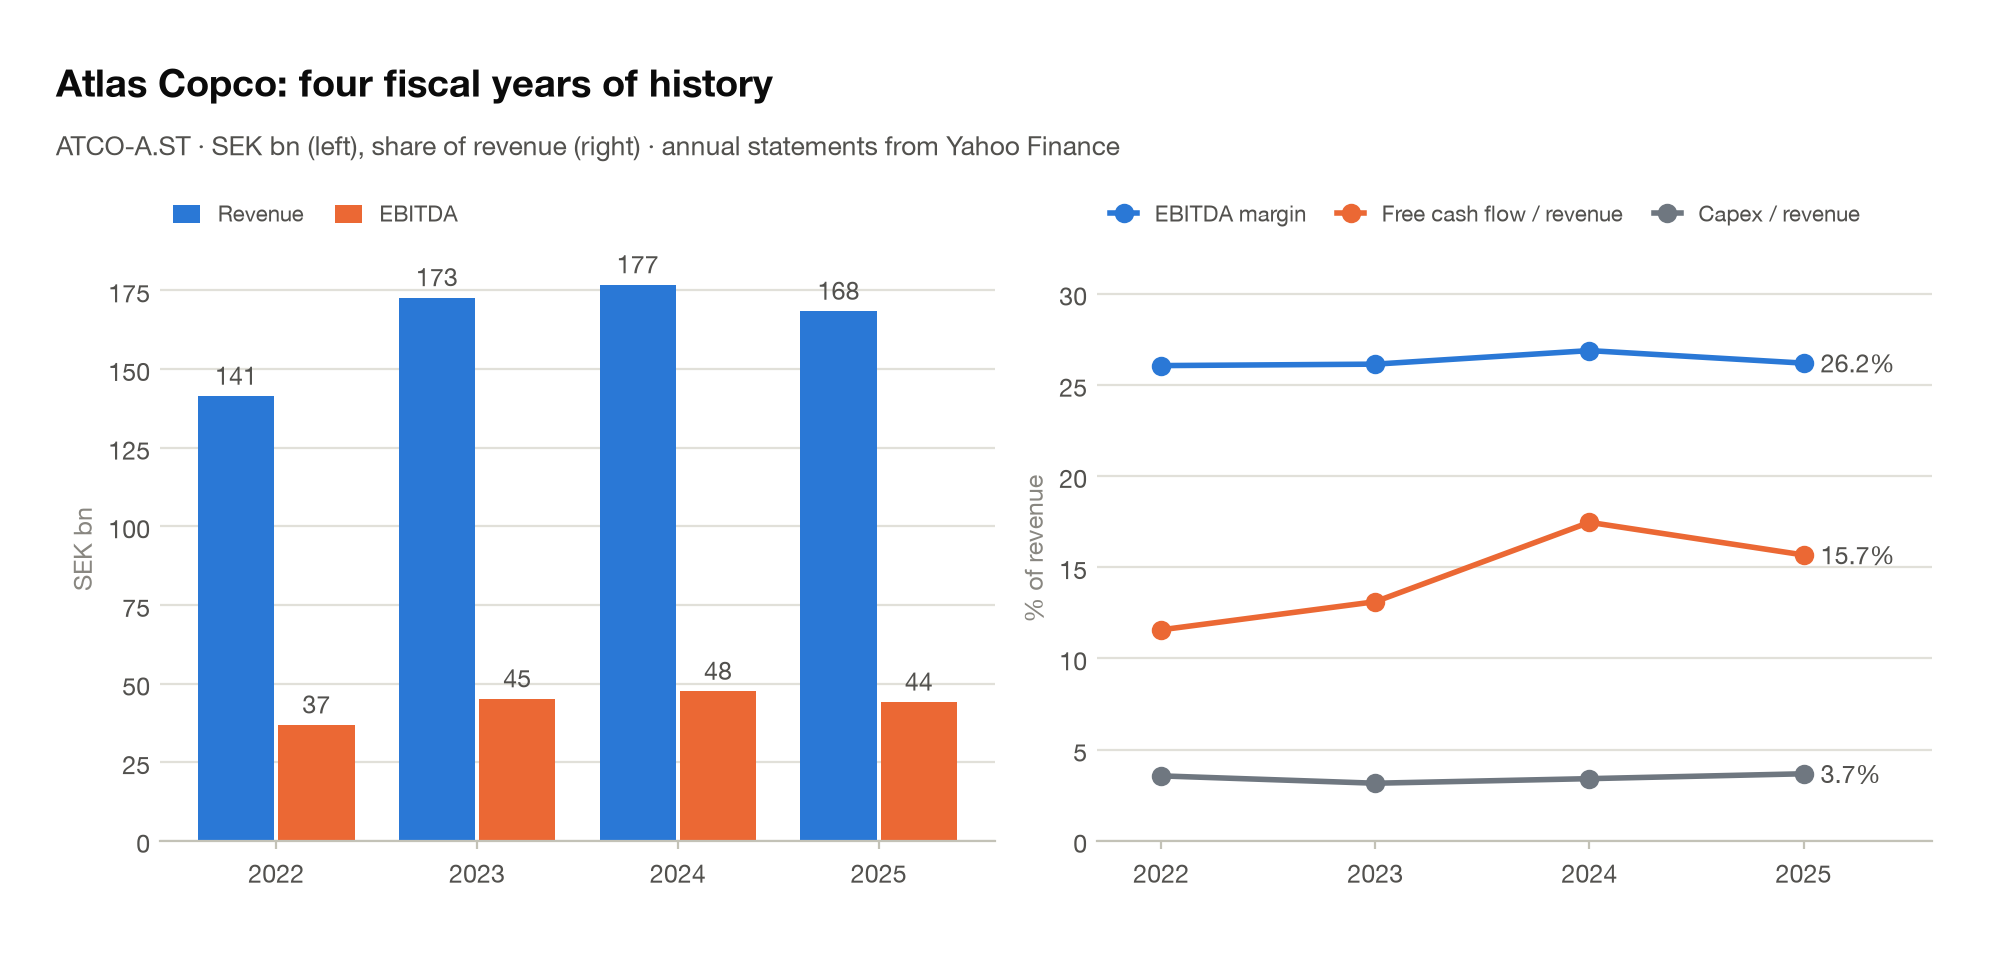
\includegraphics[width=0.95\linewidth]{history_overview.png}
\caption{Atlas Copco 2022 till 2025 enligt projektets datalager.}
\label{fig:historik}
\end{figure}

\begin{table}[ht]
\centering\small
\caption{Historiken som antagandena bygger på.}
\label{tab:historik}
\begin{tabular}{@{}lrrrr@{}}
\toprule
 & 2022 & 2023 & 2024 & 2025 \\
\midrule
Omsättning, mdkr & 141,3 & 172,7 & 176,8 & 168,3 \\
Tillväxt & & 22,2\pct & 2,4\pct & $-4,8$\pct \\
EBITDA-marginal & 26,1\pct & 26,1\pct & 26,9\pct & 26,2\pct \\
Avskrivningar / omsättning & 4,5\pct & 4,5\pct & 5,0\pct & 5,7\pct \\
Capex / omsättning & 3,6\pct & 3,2\pct & 3,4\pct & 3,7\pct \\
Rörelsekapital, smalt mått & 26,9\pct & 25,6\pct & 26,0\pct & 23,9\pct \\
Rörelsekapital, brett mått & 13,8\pct & 13,6\pct & 13,5\pct & 12,8\pct \\
Effektiv skatt & 21,8\pct & 23,0\pct & 21,2\pct & 21,5\pct \\
Förvärv, mdkr & 10,6 & 4,3 & 7,4 & 11,6 \\
\bottomrule
\end{tabular}
\end{table}

Två saker i tabell~\ref{tab:historik} styr resten. Tillväxten är ojämn: nästan hela ökningen
sedan 2022 kom under ett enda år. Och bolaget köper andra bolag för 4 till 12~mdkr om året,
vilket syns i omsättningen men inte i capex.

Tre tidpunkter blandas dessutom i datat. Kursen är från den 13 november 2026, skuld och kassa
från den 30 september 2026 och resultatet från helåret 2025. Yahoos rullande
tolvmånaderssiffror, som motorn inte använder, visar en omsättning på 176~mdkr, 4,7\pct{} över
modellens basår.

\subsection{Antagandena}

Motorns standardantaganden står i tabell~\ref{tab:prognos} och~\ref{tab:wacc}: tillväxt från
6,0\pct{} ned till 2,0\pct, marginal 26,4\pct, WACC 7,65\pct, exit-multipel 19,4. Caset prövar
vart och ett mot historiken och ändrar två:

\begin{itemize}
  \item \textbf{Rörelsekapitalet} sänks från 25,2 till 13,3\pct{} av omsättningen. Motorns smala
    mått~\eqref{eq:nwc} bortser från övriga rörelseskulder som förskott och upplupna kostnader.
    Det breda måttet ligger stabilt kring 13\pct.
  \item \textbf{Skatten} höjs från 20,6 till 21,9\pct, snittet av de tre senaste årens effektiva
    skatt. En koncern med verksamhet i många länder betalar mer än den svenska skattesatsen.
\end{itemize}

Tillväxten behålls, men den är det svagaste antagandet: 6\pct{} om året är snittet av $+22$,
$+2$ och $-5$\pct, och en del av tillväxten är köpt. WACC rörs inte, eftersom ränta och
riskpremie har namngivna källor och beta 1,13 ligger nära Yahoos egen uppgift (1,07).

\subsection{Resultaten}

\begin{table}[H]
\centering\small
\caption{Värde per aktie i kronor. ”Standard” är motorns antaganden rakt av, ”justerat” är med
de två ändringarna. Kurs 192,25\kr.}
\label{tab:resultat}
\begin{tabular}{@{}lrrrrrrr@{}}
\toprule
 & \multicolumn{3}{c}{Standard} & Bas & \multicolumn{3}{c}{Justerat} \\
\cmidrule(lr){2-4}\cmidrule(lr){6-8}
Metod & låg & bas & hög & mot kurs & låg & bas & hög \\
\midrule
DCF, Gordon-tillväxt & 93,7 & 115,8 & 153,7 & $-40$\pct & 93,6 & 115,9 & 154,1 \\
DCF, exit-multipel & 160,6 & 175,2 & 191,0 & $-9$\pct & 160,9 & 175,5 & 191,4 \\
Comps, EV/EBITDA & 152,8 & 172,9 & 190,7 & $-10$\pct & 152,8 & 172,9 & 190,7 \\
Comps, EV/Sales & 111,7 & 138,6 & 168,8 & $-28$\pct & 111,7 & 138,6 & 168,8 \\
Comps, P/E & 162,8 & 178,3 & 196,5 & $-7$\pct & 162,8 & 178,3 & 196,5 \\
LBO, betalningsförmåga & 104,4 & 117,9 & 135,3 & $-39$\pct & 104,6 & 118,2 & 135,7 \\
Monte Carlo, P10, P50, P90 & 84,3 & 116,7 & 164,9 & $-39$\pct & 83,6 & 116,9 & 165,7 \\
\bottomrule
\end{tabular}
\end{table}

Så läser du intervallen i tabell~\ref{tab:resultat} och figur~\ref{fig:football}. För DCF är
lågt värde WACC plus 1 procentenhet och tillväxt minus 0,5 (eller multipel minus 1,0), och
högt värde tvärtom. För comps är det 25:e percentilen, medianen och 75:e percentilen av
jämförelsebolagens multipel. För LBO är det priset som ger 25, 20 respektive 15\pct{}
årlig avkastning. För Monte Carlo är det 10:e, 50:e och 90:e percentilen. Under de senaste 52
veckorna har kursen rört sig mellan 149,6 och 208,3\kr.

\begin{figure}[ht]
\centering
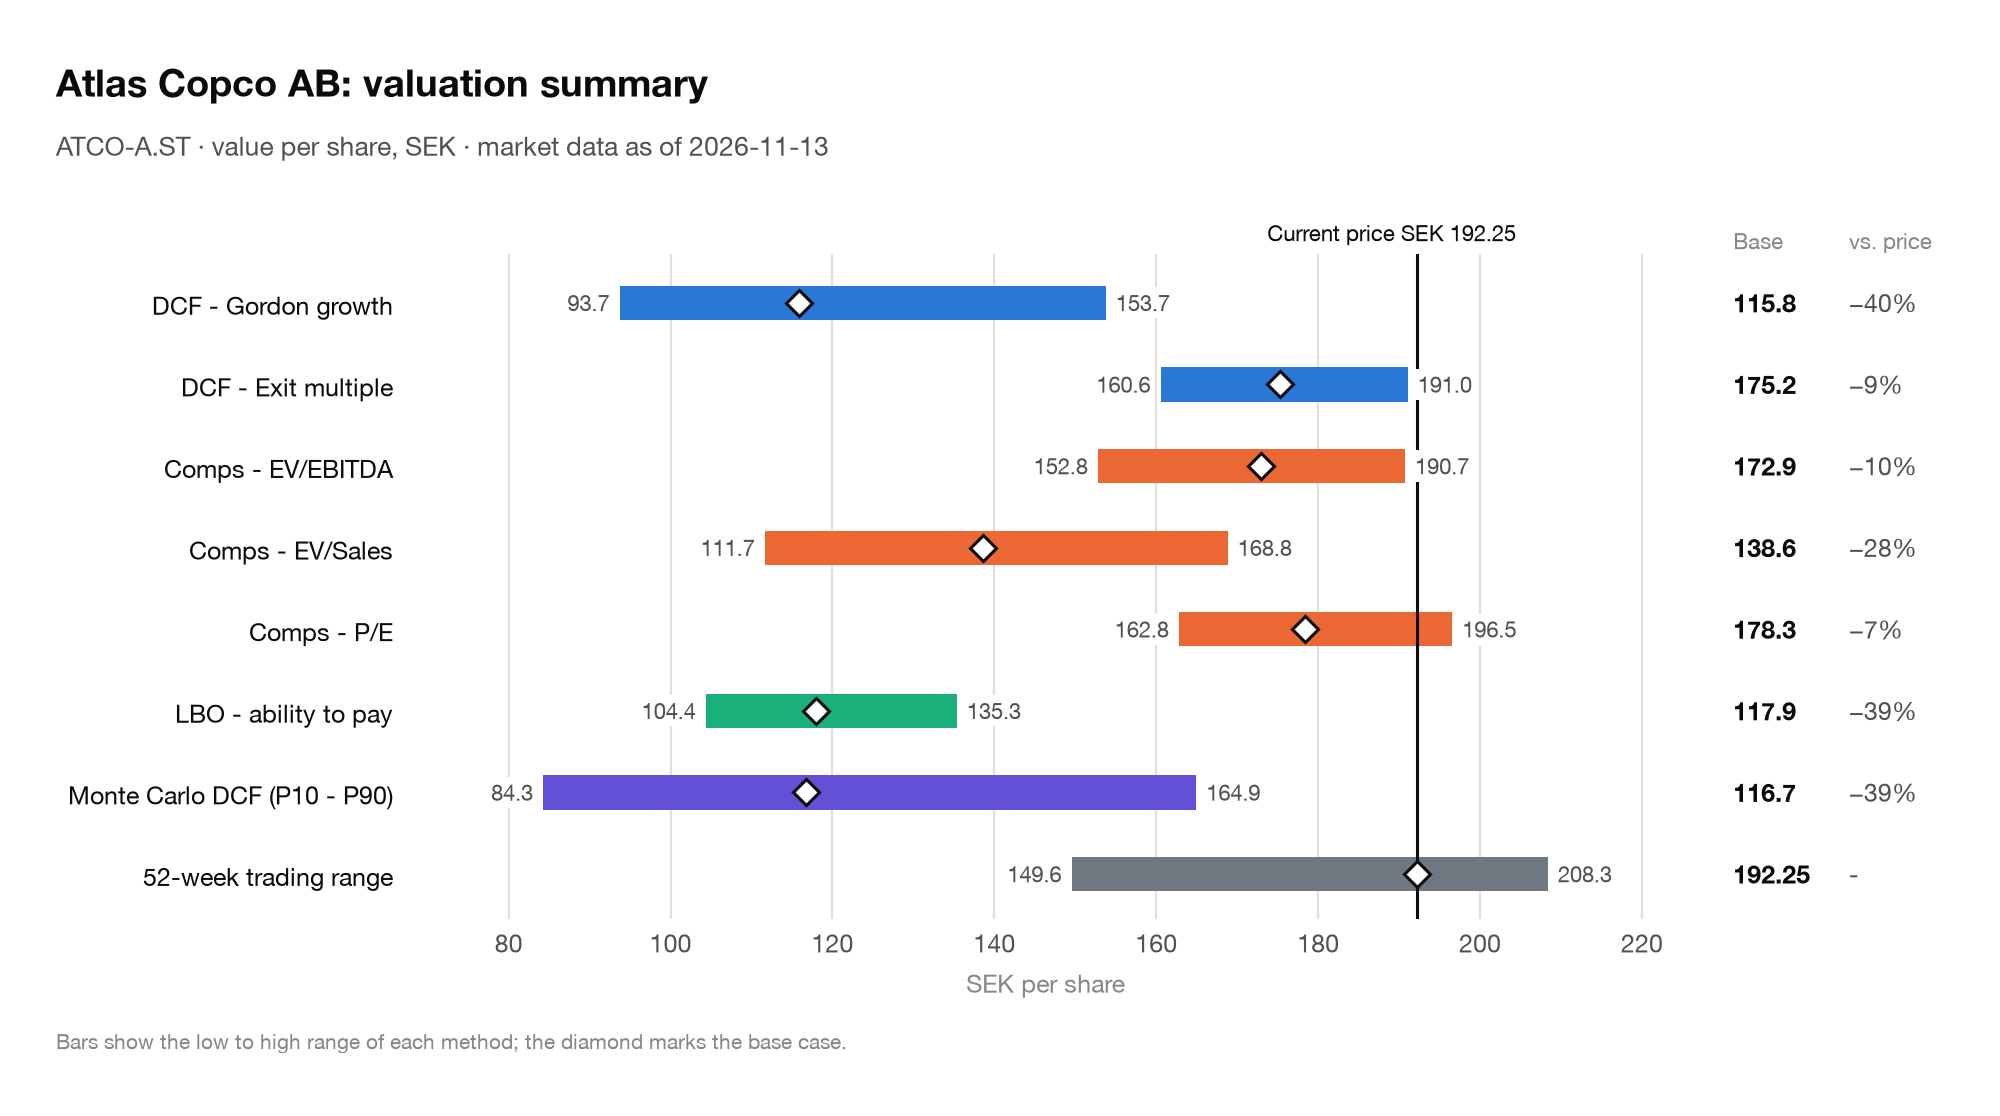
\includegraphics[width=\linewidth]{football_field.png}
\caption{Football field för Atlas Copco med standardantaganden. Staplarna är intervallet per
metod, romben basvärdet och den lodräta linjen kursen.}
\label{fig:football}
\end{figure}

De två justeringarna ändrar nästan ingenting: högre skatt sänker Gordon-värdet med ungefär
2\kr{} och lägre rörelsekapitalbindning höjer det med ungefär 2\kr. Det är i sig ett resultat.
De antaganden som går att pröva mot historiken är inte det som skiljer modellens värde från
kursen.

\subsection{Varför metoderna inte är överens}

Gordon-DCF:en säger 116\kr. Exit-DCF:en och comps säger 173 till 178\kr. Skillnaden sitter i
slutvärdet, som står för 76 till 84\pct{} av hela DCF-värdet:

\begin{itemize}
  \item Gordon-metoden antar 2\pct{} evig tillväxt. Det motsvarar att bolaget om fem år är värt
    11,7 gånger EBITDA.
  \item Exit-metoden antar att bolaget om fem år värderas som jämförelsebolagen i dag, 19,4
    gånger EBITDA. För att Gordons formel ska ge samma slutvärde krävs 4,3\pct{} evig tillväxt.
  \item Comps använder samma bolag och samma multipel direkt: 19,4 gånger EBITDA och 32,9
    gånger vinsten i median. Atlas Copco självt handlas till 21,6 och 35,5.
\end{itemize}

Exit-DCF:en och comps är alltså i grunden samma påstående: bolaget är värt vad marknaden
betalar för liknande bolag. Gordon-DCF:en är det enda oberoende måttet, och det säger att
marknadens multiplar förutsätter mer än modellen antar. Hur mycket mer? Caset räknar baklänges:
vilket värde på en drivare i taget ger exakt dagens kurs?

\begin{table}[H]
\centering\small
\caption{Vad kursen 192,25\kr{} kräver, en drivare i taget.}
\label{tab:baklanges}
\begin{tabular}{@{}lrr@{}}
\toprule
Drivare & Basfall & Krävs för värde = kurs \\
\midrule
WACC & 7,65\pct & 5,39\pct \\
Evig tillväxt & 2,0\pct & 4,6\pct \\
EBITDA-marginal & 26,4\pct & 40,0\pct \\
Snittillväxt år 1 till 5 & 4,0\pct & 16,8\pct \\
Exit-multipel (exit-metoden) & 19,4 & 21,7 \\
\bottomrule
\end{tabular}
\end{table}

Ingen enskild drivare kan rimligen flyttas så långt. Kombinationer räcker längre: WACC
6,24\pct{} tillsammans med 3,0\pct{} evig tillväxt ger precis dagens kurs, liksom 6,67\pct{} med
3,5\pct{} (figur~\ref{fig:implied}). Marknaden prissätter alltså Atlas Copco som om
avkastningskravet vore ungefär 1,4 procentenheter lägre och den eviga tillväxten 1
procentenhet högre än i modellen. Det behöver inte vara fel. En prognos som bromsar till
2\pct{} redan år fem är snål mot ett bolag med stabila marginaler: med tio års inbromsning i
stället för fem stiger Gordon-värdet från 116 till 127\kr. Modellen kan inte avgöra vem som
har rätt, bara visa vad kursen kräver.

\begin{figure}[ht]
\centering
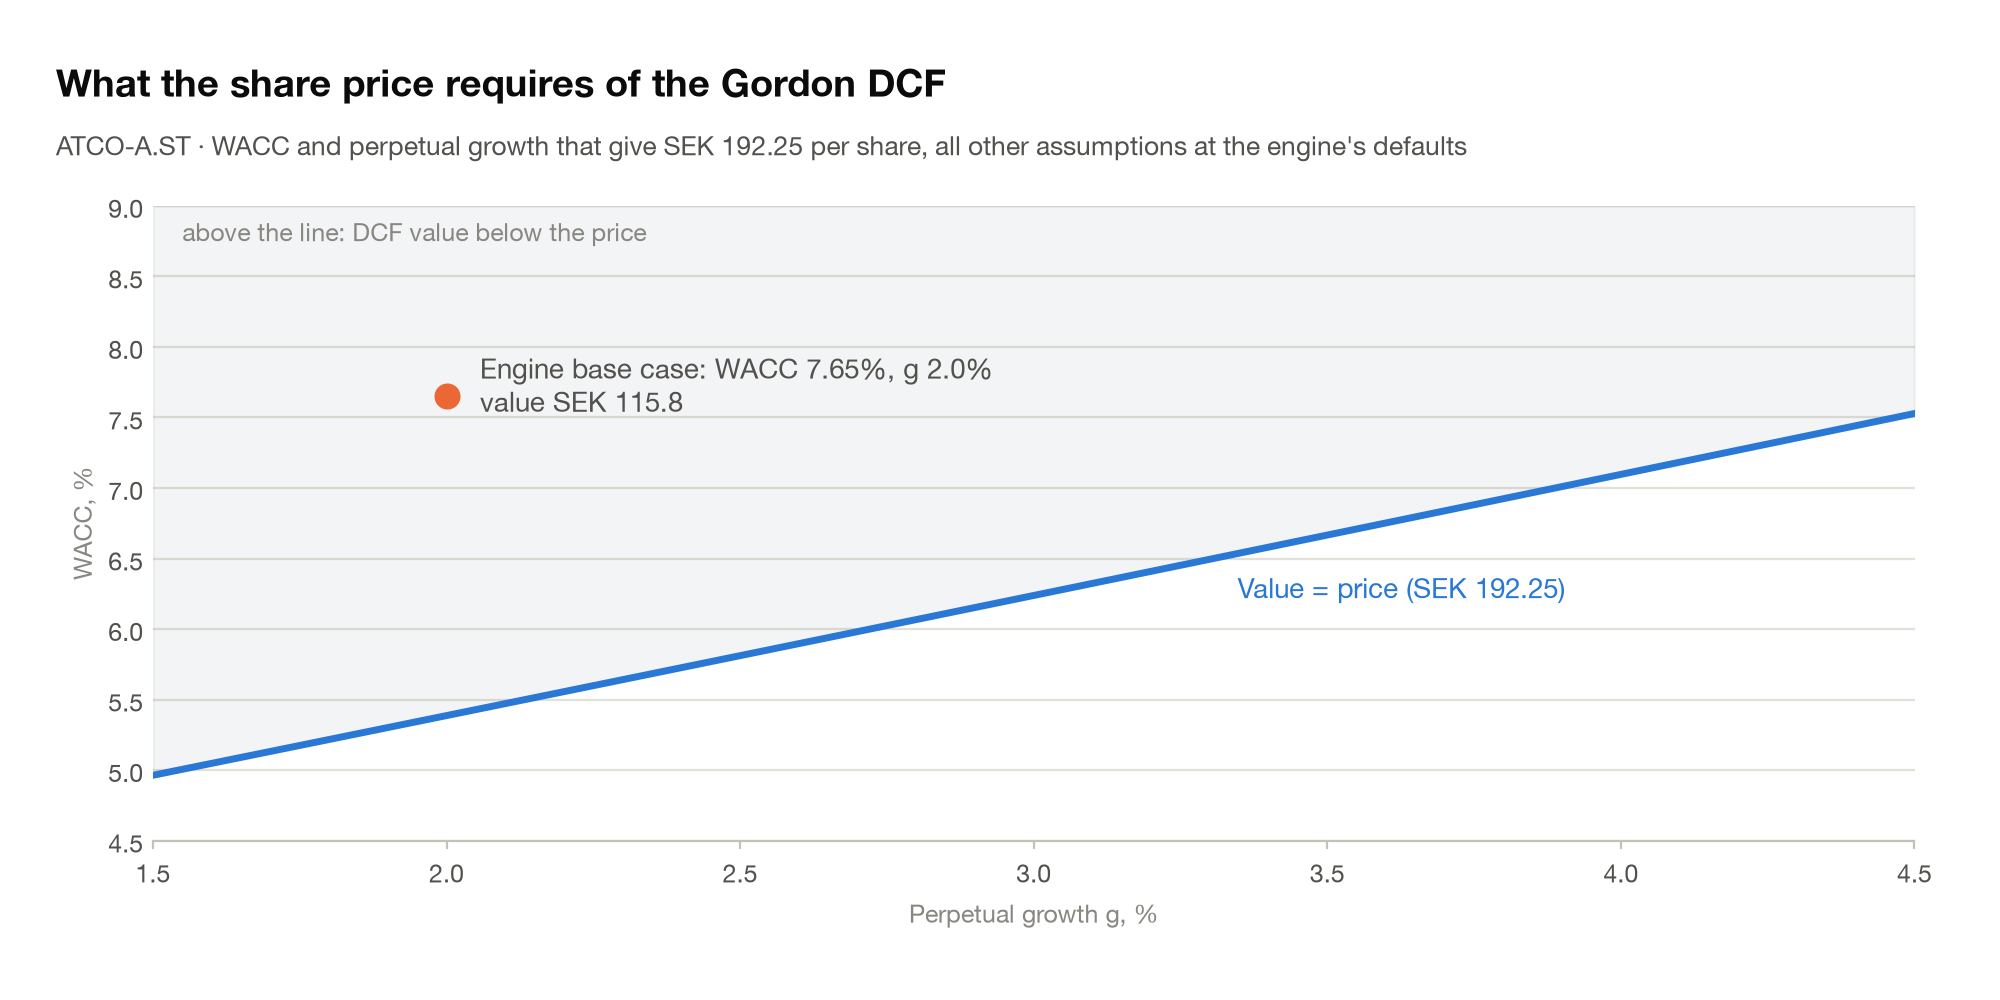
\includegraphics[width=0.9\linewidth]{implied_wacc_growth.png}
\caption{Kombinationer av WACC och evig tillväxt som ger dagens kurs.}
\label{fig:implied}
\end{figure}

De två sista metoderna har egna förklaringar. EV/Sales (139\kr) ligger lågt eftersom en
omsättningsmultipel inte tar hänsyn till att Atlas Copcos marginal (26,2\pct) är högre än
jämförelsebolagens median (21,1\pct). LBO-värdet (118\kr) ligger nära Gordon-DCF:en eftersom
det är samma kassaflöden, se avsnitt~\ref{sec:lbo}.

\subsection{Slutsatsen}

\textbf{Värdeintervall 116 till 178\kr{} per aktie mot kursen 192,25\kr.} Den nedre änden är
Gordon-DCF:ens basvärde i det justerade fallet, den övre basvärdet från P/E-comps. Caset väger
Gordon-DCF:en till 50\pct{} (den enda metoden som inte lånar sin värdering från dagens
börskurser) och comps på EV/EBITDA och P/E till 25\pct{} vardera. Tyngdpunkten blir då
146\kr. Kursen ligger 8\pct{} över intervallets övre ände och 32\pct{} över tyngdpunkten.

Övriga metoder får vikten noll, och skälen är värda att kunna. Exit-DCF:en bygger på samma
multipel som comps, så att ta med den vore att räkna comps två gånger. EV/Sales bortser från
marginalskillnaden. LBO:n är en räkneövning för ett bolag av den här storleken. Monte Carlo är
ingen egen metod utan osäkerheten kring Gordon-DCF:en.

\begin{komihag}
Vikterna är ett omdöme, inte ett resultat. Den som litar mer på marknadens prissättning av
verkstadsbolag hamnar närmare 178\kr, den som litar mer på kassaflödena närmare 116\kr. Casets
läsning är att kursen ligger över det som motorns metoder kan motivera, men inom räckhåll för
antaganden som en rimlig investerare kan ha.
\end{komihag}

\subsection{Svagheterna}

Caset är öppet med sina brister, och du ska kunna dem lika bra som siffrorna.

\begin{description}
  \item[Data.] Yahoo är gratis och det märks. Yahoos EBIT är inte bolagets rapporterade
    rörelseresultat (34,55 mot 34,11~mdkr 2025), och ingen har stämt av siffrorna mot
    årsredovisningen. Fyra bokslut är dessutom en kort historik: tillväxtantagandet vilar på
    ett enda starkt år.
  \item[Tid.] Multiplarna ställer dagens börsvärde mot ett resultat som är nästan ett år
    gammalt. Det finns ingen stubbperiod (en grov korrigering ger ungefär 2\kr{} högre värde).
  \item[Leasing och förvärv.] Leasingbetalningar finns varken i EBITDA eller i capex, vilket
    gör kassaflödena år 1 till 5 något för höga (grovt 1,5\kr{} per aktie). Den historiska
    tillväxten innehåller köpta bolag, men prognosen drar inte av några framtida förvärv.
  \item[Jämförelsebolagen.] K-means väljer $k = 2$ och gör nästan inget urval. Gruppen är
    blandad, alla bolagen är mindre än Atlas Copco, och ABB, som är större och värderas till
    22 gånger EBITDA, kom inte med.
  \item[Exit-multipeln] ärver marknadens värdering och gör exit-DCF:en till en förklädd comps.
    LBO:n säljer till samma multipel och ärver samma svaghet.
  \item[LBO:n] är inte realistisk: köparen skulle behöva över 1\,000~mdkr i eget kapital, och
    till kurs plus 30\pct{} premie blir avkastningen $-2,3$\pct{} om året.
  \item[Källbelagt och antaget.] Tre parametrar har en namngiven källa: riskfri ränta,
    riskpremie och skattesats. Allt annat är val: 2\pct{} evig tillväxt, fem års prognos,
    Blume-justeringen, storlekspremien, alla golv och tak, lånevillkoren och simuleringens
    standardavvikelser.
\end{description}

\subsection{Hela universumet}

Samma motor kördes på alla 687 bolag i Yahoos lista. Körningen tog 68 sekunder utan ett enda
oväntat fel. Av bolagen fick 294 alla fyra modellerna, 386 några av dem, och 7 saknar bokslut
hos Yahoo. Mindre än hälften får en DCF: 154 har negativ EBITDA, 103 är banker, investmentbolag
eller fastighetsbolag, och 91 har för tunn marginal för ett positivt kassaflöde.

\begin{table}[H]
\centering\small
\caption{Median av basvärde delat med kurs, per storleksklass. 1,00 betyder att metoden håller
med marknaden.}
\label{tab:universum}
\begin{tabular}{@{}lrrrrrr@{}}
\toprule
Börsvärde & Bolag & Med DCF & DCF Gordon & Comps EV/EBITDA & Comps P/E & LBO \\
\midrule
under 1 mdkr & 360 & 91 & 1,51 & 1,02 & 1,04 & 1,05 \\
1 till 5 mdkr & 124 & 66 & 1,22 & 1,00 & 0,81 & 0,82 \\
5 till 20 mdkr & 98 & 69 & 1,09 & 0,95 & 0,91 & 0,81 \\
över 20 mdkr & 98 & 70 & 0,76 & 0,95 & 0,94 & 0,66 \\
\bottomrule
\end{tabular}
\end{table}

Mönstret i tabell~\ref{tab:universum} är tydligt: DCF:en värderar småbolag högt och storbolag
lågt i förhållande till kursen, trots storlekspremien. Atlas Copcos 0,60 är alltså inget
undantag. Det talar för att gapet säger mer om modellens antaganden än om enskilda bolag:
samma 2\pct{} tillväxt och samma riskpremie för alla passar dåligt på bolag som marknaden ger
en kvalitetspremie. Att comps har median nära 1 är nästan självklart, eftersom en
relativvärdering centrerar sig kring marknaden. Som prisprognos för ett enskilt bolag duger
motorn inte. Den visar vad ett givet antagande ger och vad kursen kräver.

\section{Intervjuförberedelse}
\label{sec:intervju}

Tekniska intervjufrågor på en investmentbank är förutsägbara. Det som skiljer kandidater är
inte om de kan svaret utan om de kan ge det strukturerat på en minut. Varje svar nedan är
skrivet för att kunna sägas högt på 60 till 90 sekunder: först rubriken, sedan stegen, sist en
nyans som visar att du förstår. Frågorna står på engelska, som de ställs. Svaren står på
svenska så att du lär dig innehållet och inte en ramsa, följda av de engelska fraser du ska
kunna säga utan att tveka.

\begin{intervjutips}
Öva högt och med klocka. Börja varje svar med strukturen (”There are three steps”) och sluta
när du är klar. Om du inte kan en sak: säg vad du vet och resonera dig fram. Gissa aldrig en
siffra som om den vore säker.
\end{intervjutips}

\subsection{Redovisning}

\begin{fraga}{Walk me through the three financial statements.}
Resultaträkningen visar intäkter minus kostnader under en period och slutar i nettoresultatet.
Balansräkningen visar tillgångar, skulder och eget kapital en viss dag, och tillgångarna är
alltid lika med skulder plus eget kapital. Kassaflödesanalysen börjar med nettoresultatet,
justerar för poster som inte är betalningar och för förändringar i rörelsekapital, lägger till
investeringar och finansiering och slutar i periodens förändring av kassan. Kopplingarna:
nettoresultatet går in i kassaflödet och i eget kapital, och kassaflödets slutrad blir kassan i
balansräkningen.
\fraser{Net income flows into retained earnings and is the starting point of the cash flow
statement. The ending cash balance ties back to the balance sheet.}
\end{fraga}

\begin{fraga}{How does a 10 increase in depreciation affect the three statements?}
Resultaträkningen: resultatet före skatt faller med 10. Med 20,6\pct{} skatt faller skatten med
2,06 och nettoresultatet med 7,94. Kassaflödet: nettoresultatet är 7,94 lägre, men
avskrivningen på 10 läggs tillbaka eftersom den inte är en utbetalning, så kassaflödet från
rörelsen och kassan ökar med 2,06. Balansräkningen: anläggningstillgångarna minskar med 10 och
kassan ökar med 2,06, alltså tillgångar $-7,94$. Eget kapital minskar med 7,94 genom det lägre
resultatet. Det går ihop. Se tabell~\ref{tab:avskrivning}.
\fraser{Depreciation is a non-cash expense, so cash actually goes up by the tax shield. Both
sides of the balance sheet are down by 7.94, so it balances.}
\end{fraga}

\begin{fraga}{What is EBITDA, and why do bankers use it?}
EBITDA är rörelseresultatet före avskrivningar, räntor och skatt. Det används som en grov
approximation av rörelsens kassaflöde och för att jämföra bolag, eftersom det inte påverkas av
skuldsättning, skattesituation eller avskrivningsprinciper. Svagheten är att det bortser från
investeringar, rörelsekapital och skatt. Ett kapitalintensivt bolag kan ha hög EBITDA och ändå
lågt fritt kassaflöde. Nyansen: sedan IFRS~16 ligger leasingkostnader under EBITDA, vilket
lyfter måttet för bolag med mycket leasing.
\fraser{It is a proxy for operating cash flow that is independent of capital structure. But it
ignores capex, working capital and taxes.}
\end{fraga}

\begin{fraga}{What is the difference between unlevered and levered free cash flow?}
Det obelånade kassaflödet, FCFF, tillhör alla finansiärer: EBIT efter skatt plus avskrivningar
minus capex minus ökning av rörelsekapital. Det belånade, FCFE, är det som blir kvar till
aktieägarna efter räntor och nettoupplåning. FCFF diskonteras med WACC och ger rörelsevärdet,
FCFE med avkastningskravet på eget kapital och ger aktievärdet. I en vanlig DCF används FCFF,
eftersom man då slipper prognostisera skuldsättningen.
\fraser{Unlevered free cash flow is available to all capital providers and is discounted at the
WACC. Levered free cash flow belongs to equity holders and is discounted at the cost of
equity.}
\end{fraga}

\begin{fraga}{What is working capital, and how does a change in it affect cash flow?}
Rörelsekapital är omsättningstillgångar minus kortfristiga rörelseskulder, i sin enklaste form
kundfordringar plus lager minus leverantörsskulder. En ökning binder pengar och är ett
kassautflöde: om lagret ökar med 10 har bolaget betalat 10 som ännu inte syns som kostnad.
Växande bolag behöver därför normalt finansiera sitt rörelsekapital. Bolag som får betalt i
förskott kan ha negativt rörelsekapital, och då frigör tillväxten pengar.
\fraser{An increase in net working capital is a use of cash.}
\end{fraga}

\subsection{DCF och WACC}

\begin{fraga}{Walk me through a DCF.}
En DCF värderar ett bolag som nuvärdet av dess framtida kassaflöden. Fem steg. Ett: prognostisera
det obelånade fria kassaflödet i fem till tio år. Två: beräkna WACC. Tre: beräkna ett slutvärde
för tiden efter prognosen, med Gordons formel eller en exit-multipel. Fyra: diskontera
kassaflödena och slutvärdet med WACC och summera till rörelsevärdet. Fem: dra av nettoskuld och
minoritetsintressen för att få aktievärdet, och dela med antalet aktier. Avsluta med en
känslighetsanalys på WACC och tillväxt, eftersom slutvärdet oftast är det mesta av värdet.
\fraser{I project unlevered free cash flows, discount them at the WACC, add a terminal value,
and bridge from enterprise value to equity value.}
\end{fraga}

\begin{fraga}{What is WACC and how do you calculate it?}
WACC är det vägda avkastningskravet från alla som finansierar bolaget och används som
diskonteringsränta för FCFF. Det är andelen eget kapital gånger avkastningskravet på eget
kapital, plus andelen skuld gånger låneräntan efter skatt, se~\eqref{eq:wacc}. Vikterna är
marknadsvärden. Avkastningskravet på eget kapital kommer från CAPM. Låneräntan multipliceras
med ett minus skattesatsen eftersom räntan är avdragsgill. För Atlas Copco fick jag 7,65\pct:
96\pct{} eget kapital till 7,84\pct{} och 4\pct{} skuld till 2,84\pct{} efter skatt.
\fraser{Cost of equity times the equity weight, plus after-tax cost of debt times the debt
weight, using market values.}
\end{fraga}

\begin{fraga}{How do you calculate the cost of equity?}
Med CAPM: riskfri ränta plus beta gånger marknadens riskpremie. Den riskfria räntan är en lång
statsobligation i samma valuta som kassaflödena, här den svenska tioåringen på 3,075\pct.
Riskpremien är vad aktiemarknaden väntas ge utöver det. Jag använde Damodarans 4,23\pct{} för
Sverige. Beta mäter aktiens känslighet för marknaden. Tanken är att investerare bara får
betalt för risk som inte kan diversifieras bort. Nyansen: riskpremien går inte att observera,
och ett annat källval ger ett annat värde.
\fraser{Risk-free rate plus beta times the equity risk premium. Only systematic risk is
compensated.}
\end{fraga}

\begin{fraga}{What is beta, and how do you unlever and relever it?}
Beta är lutningen i en regression av aktiens avkastning på marknadens, kovariansen delat med
marknadens varians. Ett observerat beta speglar både rörelsens risk och skuldsättningen. För
att låna beta från jämförelsebolag rensar man därför först bort deras skuldsättning: beta delat
med ett plus ett minus skattesatsen gånger skuld genom eget kapital. Man tar medianen och
lägger sedan på målbolagets egen kapitalstruktur med samma formel baklänges,
se~\eqref{eq:hamada}. Skälet att använda jämförelsebolag är att ett enskilt regressionsbeta är
brusigt.
\fraser{Unlevered beta equals levered beta divided by one plus one minus the tax rate times
debt to equity. Then I relever at the target's capital structure.}
\end{fraga}

\begin{fraga}{How do you calculate terminal value, and which method do you prefer?}
Två metoder. Gordons formel antar evig tillväxt: nästa års kassaflöde delat med WACC minus
tillväxt. Exit-multipeln antar att bolaget säljs sista prognosåret till en multipel av EBITDA.
Jag räknar alltid båda och stämmer av dem mot varandra: vilken multipel motsvarar min tillväxt,
och vilken tillväxt motsvarar min multipel? I mitt case gav 2\pct{} tillväxt en multipel på
11,7 gånger, medan jämförelsebolagens 19,4 gånger motsvarade 4,3\pct{} evig tillväxt. Den
skillnaden var hela förklaringen till att metoderna inte var överens.
\fraser{The perpetuity growth method and the exit multiple method. I cross-check one against the
other through the implied multiple and the implied growth rate.}
\end{fraga}

\begin{fraga}{What is the mid-year convention?}
En vanlig DCF diskonterar varje års kassaflöde som om det kom vid årets slut. I verkligheten
kommer det löpande under året, i snitt vid halvårsskiftet. Halvårskonventionen diskonterar
därför år $t$ med $t$ minus ett halvt år, vilket höjer värdet något. Det viktiga är
slutvärdet: Gordon-värdet ska också justeras upp med ett halvt års ränta, medan ett slutvärde
från en exit-multipel avser en försäljning vid årets slut och inte ska justeras.
\fraser{Cash flows arrive evenly through the year, so I discount them at t minus one half. The
exit multiple terminal value gets no mid-year adjustment.}
\end{fraga}

\begin{fraga}{What is the difference between enterprise value and equity value?}
Rörelsevärdet är värdet av hela rörelsen för alla finansiärer, oavsett hur den är finansierad.
Aktievärdet är det som tillhör aktieägarna. Bryggan: rörelsevärde minus nettoskuld, minus
minoritetsintressen och preferensaktier, är aktievärde. Åt andra hållet: börsvärde plus
nettoskuld är rörelsevärde. Rörelsevärdet används med mått före räntor, som EBITDA, och
aktievärdet med mått efter räntor, som nettoresultat.
\fraser{Enterprise value is the value of the operations to all investors. Equity value is what
is left for shareholders after net debt and other claims.}
\end{fraga}

\begin{fraga}{Why do you subtract cash and add minority interest when you calculate enterprise value?}
Kassan dras av eftersom den inte behövs i rörelsen: en köpare som betalar för aktierna får
kassan med på köpet och kan använda den till att betala skulden. Minoritetsintressen läggs
till eftersom koncernens EBITDA räknas till 100\pct{} även för dotterbolag som delvis ägs av
andra. Täljaren måste då också innehålla hela värdet, annars jämför man äpplen med päron.
\fraser{Cash is a non-operating asset. Minority interest is added for consistency, because
consolidated EBITDA includes one hundred percent of the subsidiary.}
\end{fraga}

\begin{fraga}{Which has a bigger impact on a DCF: the discount rate or the growth rate?}
Båda verkar genom samma nämnare, WACC minus tillväxt, så en procentenhet i den ena är ungefär
lika mycket värd som en procentenhet i den andra för slutvärdet. Men WACC påverkar dessutom
diskonteringen av alla kassaflöden, så WACC väger normalt något tyngre. Det avgörande är hur
liten nämnaren är. I mitt case var den 5,65 procentenheter, och då sänker en procentenhet högre
WACC slutvärdet med omkring 15\pct.
\fraser{The value is driven by the spread between the WACC and the growth rate. The smaller the
spread, the more sensitive the valuation.}
\end{fraga}

\begin{fraga}{Terminal value is 80 percent of your DCF. Is that a problem?}
Det är normalt för ett moget bolag med fem års prognos, och i mitt case var andelen 76 till
84\pct. Men det betyder att värderingen står och faller med två eller tre antaganden om tiden
efter år fem. Jag hanterar det på tre sätt: stämmer av de två slutvärdesmetoderna mot varandra,
visar en känslighetstabell, och räknar baklänges vad marknadspriset kräver. En längre
prognosperiod minskar andelen men flyttar bara osäkerheten.
\fraser{That is typical, and it is exactly why I sanity-check the implied multiple and run
sensitivities.}
\end{fraga}

\begin{fraga}{Does more debt always lower the WACC?}
Nej. Skuld är billigare än eget kapital och räntan är avdragsgill, så lite skuld sänker WACC.
Men mer skuld gör aktien mer riskfylld: beta stiger enligt Hamada, och därmed avkastningskravet
på eget kapital. Vid hög skuldsättning stiger också låneräntan och risken för finansiella
problem. WACC är därför U-formad i skuldsättningen. Utan skatter och konkurskostnader tar
effekterna ut varandra helt. Det är Modigliani och Millers resultat.
\fraser{Debt is cheaper and tax-deductible, but it raises the cost of equity and eventually the
cost of debt. There is an optimal capital structure.}
\end{fraga}

\subsection{Multiplar och metodval}

\begin{fraga}{What are the main valuation methods, and which gives the highest value?}
Tre huvudmetoder: DCF, som ger ett fristående värde ur kassaflödena, jämförelsebolag, som visar
vad börsen betalar för liknande bolag, och jämförbara transaktioner \en{precedent transactions},
som visar vad köpare har betalat för hela bolag. Därtill LBO-analys. Som tumregel ger
transaktioner högst värde, eftersom priserna innehåller en kontrollpremie, och LBO lägst,
eftersom en finansiell köpare kräver hög avkastning. DCF kan hamna var som helst beroende på
antagandena. Mitt projekt har inte transaktionsmultiplar, eftersom det saknas gratis data.
\fraser{DCF, trading comps and precedent transactions. Precedents usually come out highest
because they include a control premium.}
\end{fraga}

\begin{fraga}{When would you use EV/EBITDA rather than P/E?}
EV/EBITDA när jag vill jämföra rörelser oberoende av finansiering: måttet påverkas inte av
skuldsättning, skatt eller avskrivningsprinciper, och det är standard för industribolag och i
transaktioner. P/E när kapitalstrukturen är en del av verksamheten, framför allt banker och
försäkringsbolag, där rörelsevärde och EBITDA inte är meningsfulla. P/E är också det mått
aktieinvesterare oftast tittar på. Viktigast är att inte blanda: rörelsevärde hör ihop med
resultat före räntor, börsvärde med resultat efter räntor.
\fraser{EV/EBITDA is capital structure neutral. P/E is an equity multiple and is affected by
leverage.}
\end{fraga}

\begin{fraga}{How do you select comparable companies?}
Jag letar efter bolag med samma affärsmodell och samma drivkrafter: bransch och geografi först,
sedan storlek, tillväxt, marginaler och risk. Hellre fem bra jämförelsebolag än femton
dåliga. Sedan rensar jag uteliggare och tittar på median och kvartiler, inte medelvärde. I mitt
projekt gjorde en algoritm urvalet inom sektorn, och det lärde mig var gränsen går: den
hittade rimliga bolag men kan inte veta att två bolag med samma nyckeltal säljer helt olika
saker.
\fraser{Same industry and business model first, then size, growth, margins and risk. I use the
median rather than the mean.}
\end{fraga}

\begin{fraga}{Why would two similar companies trade at different multiples?}
En multipel är en hoptryckt DCF: den bestäms av tillväxt, risk och hur mycket av resultatet som
blir kassaflöde, se~\eqref{eq:multipel-dcf}. Högre väntad tillväxt, lägre risk eller högre
avkastning på kapitalet motiverar en högre multipel. Därutöver kan skillnaden vara teknisk:
olika redovisning, engångsposter i resultatet eller olika perioder. Först när allt det är
uteslutet kan man säga att ett av bolagen är felprissatt.
\fraser{Differences in growth, risk and returns on capital. A multiple is shorthand for a DCF.}
\end{fraga}

\begin{fraga}{A company has negative earnings. How do you value it?}
P/E fungerar inte, och är EBITDA också negativ faller EV/EBITDA bort. Då återstår
omsättningsmultiplar, med reservationen att de bortser från lönsamheten, och en DCF med en
uttalad väg till lönsamhet. En sådan DCF är mycket känslig för när och på vilken nivå
marginalen stabiliseras. Min motor avstår helt från DCF vid negativ EBITDA, eftersom den bara
kan skriva fram historiken, och det gällde 154 av 687 svenska bolag. Hellre det än ett tal
utan mening.
\fraser{I would look at revenue multiples and a DCF with an explicit path to profitability, and
be clear about the uncertainty.}
\end{fraga}

\begin{fraga}{How would you value a bank?}
Inte med en vanlig DCF. För en bank är skulden råvaran, inte finansieringen: inlåning och
upplåning är en del av rörelsen, så rörelsevärde, EBITDA och FCFF saknar mening. Man värderar
i stället det egna kapitalet direkt, med P/E och kurs mot eget kapital (P/B) ställt mot
avkastningen på eget kapital, eller med en utdelningsmodell där utdelningarna diskonteras med
avkastningskravet på eget kapital. Min motor ger banker bara P/E, och säger det öppet.
\fraser{For a bank, debt is a raw material rather than a source of financing, so I use equity
multiples like P/E and price to book, or a dividend discount model.}
\end{fraga}

\begin{fraga}{What is a football field chart?}
Ett diagram med en liggande stapel per värderingsmetod som visar metodens intervall för värde
per aktie, och en lodrät linje för aktuell kurs eller ett bud. Det används i pitchar och i
underlag till styrelser för att visa var metoderna överlappar. Poängen är inte ett exakt tal
utan ett försvarbart intervall. Man ska kunna förklara varje stapels ändpunkter och varför
staplarna ligger där de gör.
\fraser{It summarises the valuation ranges from each methodology side by side, against the
current share price.}
\end{fraga}

\subsection{LBO}

\begin{fraga}{Walk me through an LBO.}
I en LBO köper ett riskkapitalbolag ett bolag med en stor andel lånade pengar. Stegen: ett,
anta ett köppris, oftast som multipel av EBITDA. Två, bestäm finansieringen i en uppställning
av källor och användning: lån i olika skikt och resten eget kapital. Tre, prognostisera
kassaflödet och använd det till ränta och amortering. Fyra, anta en försäljning efter omkring
fem år till en exit-multipel, dra av kvarvarande skuld och få ägarens likvid. Fem, räkna IRR
och MOIC på ägarens insats. Ofta vänder man på det och löser ut det pris som ger ett visst
avkastningskrav.
\fraser{Purchase price, sources and uses, debt paydown from free cash flow, exit, and then the
sponsor's IRR and multiple of money.}
\end{fraga}

\begin{fraga}{Why does an LBO use debt?}
Hävstång. Skuld är billigare än eget kapital, och om bolaget är värt mer än skulden vid
försäljningen tillfaller hela värdeökningen ägaren, som bara har satsat en del av köpeskillingen.
Samma värdeökning på en mindre insats ger högre avkastning. Dessutom är räntan avdragsgill, och
kravet att betala ränta tvingar fram disciplin i bolaget. Baksidan är risken: skulden ska
betalas även om resultatet faller, och då är det ägarens kapital som försvinner först.
\fraser{Leverage amplifies equity returns, and interest is tax-deductible. The trade-off is
financial risk.}
\end{fraga}

\begin{fraga}{What drives returns in an LBO?}
Tre saker. Resultattillväxt: bolaget säljs med högre EBITDA än det köptes med. Multipelexpansion:
det säljs till en högre multipel än köpet. Amortering: bolagets kassaflöde betalar ned skulden,
så en större del av rörelsevärdet tillhör ägaren. De tre summerar exakt till värdeskapandet
efter avgifter, se~\eqref{eq:attribution}. Den mest pålitliga källan är amorteringen och den
minst pålitliga multipeln. I mitt case köptes bolaget till 28 gånger EBITDA och såldes till 19,
och multipelfallet åt upp allt annat.
\fraser{EBITDA growth, multiple expansion and debt paydown.}
\end{fraga}

\begin{fraga}{What makes a good LBO candidate?}
Ett bolag som klarar skuld: stabila och förutsägbara kassaflöden, låga investeringsbehov, lågt
rörelsekapitalbehov, stark marknadsposition och låg befintlig skuldsättning. Det ska gå att
köpa till en rimlig multipel, det ska finnas förbättringsmöjligheter i rörelsen, och det ska
finnas en trolig väg ut om några år, till en industriell köpare, en annan fond eller börsen.
Cykliska bolag och bolag med stora investeringsbehov passar sämre.
\fraser{Stable cash flows, low capex requirements, a strong market position and a clear exit
route.}
\end{fraga}

\begin{fraga}{What is the difference between IRR and MOIC?}
MOIC är pengar ut delat med pengar in och bryr sig inte om tiden. IRR är den årliga avkastning
som gör nuvärdet av alla ägarens kassaflöden till noll. Med en insats och en utbetalning är
IRR lika med MOIC upphöjt till ett genom antalet år, minus ett. Dubbla pengarna är 26\pct{} om
året på tre år men 15\pct{} på fem. En tidig utdelning höjer IRR utan att höja MOIC, och därför
tittar investerare på båda.
\fraser{MOIC tells you how much, IRR tells you how fast. Two times your money in five years is
roughly a fifteen percent IRR.}
\end{fraga}

\begin{fraga}{What is the difference between senior and subordinated debt, and what is a cash sweep?}
Seniora lån har förmånsrätt: de betalas först vid en konkurs och har ofta säkerhet i bolagets
tillgångar. De har därför lägre ränta, amorteras löpande och har hårdare villkor. Efterställda
lån står längre bak i kön, har högre ränta och betalas ofta i en klump vid förfall. Ett
\en{cash sweep} betyder att överskottskassa, utöver den obligatoriska amorteringen, används
till att betala det seniora lånet i förtid. Det sänker räntekostnaden och risken, och det
ökar ägarens andel av värdet.
\fraser{Senior debt ranks first and is cheaper. A cash sweep uses excess cash flow to prepay
senior debt.}
\end{fraga}

\subsection{Omdöme}

\begin{fraga}{Your DCF says 116 and the stock trades at 192. Who is right?}
Det kan modellen inte avgöra, och jag skulle inte påstå det. Det den kan säga är vad kursen
förutsätter. Jag räknade baklänges: kursen kräver ungefär 1,4 procentenheter lägre
avkastningskrav och en procentenhet högre evig tillväxt än jag antog. Det är inte orimligt för
ett kvalitetsbolag, och min modell är snål: den bromsar tillväxten till 2\pct{} redan år fem.
Samtidigt såg jag samma mönster i hela universumet, där DCF:en värderar storbolag till 0,76
av kursen i median. Det tyder på att gapet säger mer om modellens antaganden än om just det
här bolaget.
\fraser{A DCF does not tell you the price is wrong. It tells you what you need to believe for
the price to be right.}
\end{fraga}

\subsection{Att presentera projektet på en minut}

Du kommer att få frågan ”tell me about something you have built” eller ”walk me through a
project on your CV”. Svaret ska vara på engelska, ta en minut och sluta i en insikt, inte i en
lista över tekniker.

\begin{tcolorbox}[enhanced,colback=accent!4,colframe=accent,boxrule=0.5pt,arc=2pt,
  left=10pt,right=10pt,top=8pt,bottom=8pt,title={The pitch (about 60 seconds)},
  fonttitle=\sffamily\bfseries\small,coltitle=white,colbacktitle=accent,
  before upper={\setlength{\parskip}{0.5\baselineskip}}]
\begin{english}
I built a valuation engine in Python that values every
Swedish listed company on Yahoo Finance, 687 of them, the way a bank would: a DCF with a
CAPM-based WACC, trading comps, an LBO and a Monte Carlo simulation, summarised in a football
field and exported to Excel.

I then used it for a case study on Atlas Copco. The interesting result was not a price target
but a disagreement. The DCF with two percent terminal growth gives about 116 kronor per share.
Comps and the exit-multiple DCF give around 175. The stock trades at 192. I traced the gap to
the terminal value: the peer multiple of 19 times EBITDA implies more than four percent growth
forever. So the model cannot tell you who is right, but it shows exactly what the market price
assumes.

What I learned most from was where the mechanical approach breaks. For example, the clustering
barely selects peers on its own, and the Monte Carlo range mostly reflects the volatilities I
assumed.
\end{english}
\end{tcolorbox}

\paragraph{Varför den fungerar.} Den börjar med vad projektet \emph{är} i en mening, med
siffror som visar omfånget. Den går sedan till ett resultat som kräver förståelse (varför
metoderna är oense), inte till en uppräkning av bibliotek. Och den slutar med svagheter som du
själv har hittat. Det sista är det viktigaste: den som intervjuar har sett många DCF-modeller,
men få kandidater som självmant säger var deras modell är svag.

\paragraph{Följdfrågor du ska räkna med, och ärliga svar.}

\begin{description}
  \item[”Would you buy the stock?”] Nej, inte på det här underlaget. Modellen är ett läroexempel
    på gratis data som inte är avstämda mot årsredovisningen. Den visar vad kursen kräver,
    inte om kursen är fel.
  \item[”Why k-means? Did it work?”] Bara delvis. Den valde två kluster, och 119 av 148
    kandidater hamnade i samma som Atlas Copco. Urvalet görs i praktiken av närmaste grannar
    inom sektorn med förtur för samma bransch. En analytiker hade valt för hand, och ABB hade
    troligen kommit med.
  \item[”Where does your size premium come from?”] Det är ett eget antagande, inte skattat ur
    data och inte källbelagt. Det finns där för att regressionsbeta för illikvida småbolag blir
    för låg. Det går att stänga av, och i caset är premien noll.
  \item[”What does the Monte Carlo actually tell you?”] Hur känslig modellen är för sina egna
    indata. Bredden bestäms av standardavvikelser som jag har antagit, och tillväxtens bygger
    på tre observationer. Att 3,3\pct{} av dragningarna ligger över kursen är ingen sannolikhet
    för att aktien är undervärderad.
  \item[”What would you do next?”] Rullande tolvmånaderssiffror i stället för senaste bokslut,
    en stubbperiod, justering för leasing, kurs mot eget kapital för banker och fastighetsbolag,
    transaktionsmultiplar, och framför allt en avstämning av indata mot bolagens egna rapporter.
\end{description}

\section{Appendix: övningar och ordlista}
\label{sec:appendix}

\subsection{Övningar med lösningar}

Övningarna följer kapitlen. De flesta löser du med penna och papper, några genom att köra
motorn. Kommandona förutsätter att du står i repots rot med den virtuella miljön aktiverad.
Alla körs offline och ger därför exakt de tal som står i lösningarna.

\subsubsection*{Redovisning}

\begin{ovning}[penna och papper]
Ett bolag köper en maskin för 100\kr{} kontant den 1 januari och skriver av den linjärt på
fem år. Skattesatsen är 20,6\pct. Hur påverkas de tre rapporterna det första året?
\end{ovning}
\begin{losning}
Avskrivningen är 20. Resultaträkning: resultat före skatt $-20$, skatt $+4,12$, nettoresultat
$-15,88$. Kassaflöde: rörelsen $-15,88 + 20 = +4,12$, investeringar $-100$, kassan $-95,88$.
Balansräkning: anläggningstillgångar $+100 - 20 = +80$, kassa $-95,88$, alltså tillgångar
$-15,88$, och eget kapital $-15,88$. Det går ihop. Lägg märke till att själva köpet inte syns
i resultaträkningen.
\end{losning}

\begin{ovning}[penna och papper]
Ett bolag har EBIT 200, avskrivningar 50, capex 70, en ökning av rörelsekapitalet på 10,
räntekostnader 30 och ökar sina lån med 20 netto. Skattesatsen är 20,6\pct. Beräkna FCFF och
FCFE.
\end{ovning}
\begin{losning}
Enligt~\eqref{eq:fcff}: $\FCFF = 200 \cdot 0,794 + 50 - 70 - 10 = 128,8$.
Enligt~\eqref{eq:fcfe}: $\FCFE = 128,8 - 30 \cdot 0,794 + 20 = 125,0$.
\end{losning}

\subsubsection*{DCF}

\begin{ovning}[penna och papper]
Nästa års kassaflöde är 100, WACC 8\pct{} och evig tillväxt 2\pct. (a) Beräkna slutvärdet. (b)
Hur ändras det om $g$ är 3\pct, respektive om WACC är 9\pct? (c) Hur stor del av värdet kommer
från kassaflöden mer än 20 år bort?
\end{ovning}
\begin{losning}
(a) $100 / 0,06 = 1\,667$. (b) $100 / 0,05 = 2\,000$, alltså $+20$\pct, respektive
$100 / 0,07 = 1\,429$, alltså $-14$\pct. (c) Summan av termerna efter de $n$ första i den
geometriska serien~\eqref{eq:gordon} är andelen $q^n$ av helheten, med
$q = 1,02 / 1,08 = 0,944$. För $n = 20$ blir det $0,944^{20} = 0,32$. En tredjedel av
slutvärdet kommer alltså från år som ligger mer än två decennier efter prognosens slut.
\end{losning}

\begin{ovning}[penna och papper]
Ett bolag ger kassaflödet 100 om året i tre år. Därefter växer kassaflödet med 2\pct{} om året
för alltid, med början på 102 år fyra. WACC är 10\pct. Beräkna rörelsevärdet (a) med
årsslutskonvention och (b) med halvårskonvention. (c) Vad är kvoten mellan svaren, och varför?
\end{ovning}
\begin{losning}
(a) Prognosåren: $100\,(1,1^{-1} + 1,1^{-2} + 1,1^{-3}) = 248,7$. Slutvärde:
$102 / 0,08 = 1\,275$, nuvärde $1\,275 / 1,1^3 = 957,9$. Summa $1\,206,6$. (b) Prognosåren:
$100\,(1,1^{-0,5} + 1,1^{-1,5} + 1,1^{-2,5}) = 260,8$. Slutvärdet får faktorn $1,1^{0,5}$:
$1\,275 \cdot 1,0488 / 1,1^3 = 1\,004,7$. Summa $1\,265,5$. (c) Kvoten är $1,0488 = 1,1^{0,5}$.
Med Gordon-slutvärde flyttar halvårskonventionen \emph{alla} kassaflöden ett halvår närmare,
så hela värdet multipliceras med $(1+r)^{1/2}$. Med exit-multipel gäller det bara prognosåren.
\end{losning}

\begin{ovning}[kör motorn]
Stäng av capex-golvet i slutåret för Atlas Copco. Vad blir Gordon-värdet och den implicita
multipeln? Kontrollera kassaflödet år $N+1$ för hand med~\eqref{eq:terminal-fcff}.
\begin{lstlisting}
from valuation_engine.pipeline import run_valuation
from valuation_engine.models import dcf

d = run_valuation("ATCO-A.ST", offline=True).dcf
out = dcf.dcf_core(**{**d.core_inputs, "terminal_capex_floor": False})
print(out.value_per_share_gordon[0], out.implied_exit_multiple[0], out.terminal_fcff[0] / 1e9)
\end{lstlisting}
\end{ovning}
\begin{losning}
Utskriften är 124,69\kr{} per aktie, multipeln 12,8 och kassaflödet 37,78~mdkr (mot 115,85,
11,7 och 34,38 med golvet). För hand: utan golv är
$u = 0,2135 \cdot 0,794 + 0,0504 - 0,0341 = 0,1859$ och
$\FCFF_{N+1} = 204,7 \cdot (1,02 \cdot 0,1859 - 0,2516 \cdot 0,02) = 37,8$. Golvet kostar
alltså ungefär 9\kr{} per aktie.
\end{losning}

\subsubsection*{WACC och beta}

\begin{ovning}[penna och papper]
Ett bolag har börsvärde 800 och skuld 200. Beta är 1,2, den riskfria räntan 3,075\pct,
riskpremien 4,23\pct, låneräntan 5\pct{} och skattesatsen 20,6\pct. Beräkna WACC.
\end{ovning}
\begin{losning}
$r_e = 3,075 + 1,2 \cdot 4,23 = 8,15$\pct. Låneränta efter skatt: $5 \cdot 0,794 = 3,97$\pct.
$\WACC = 0,8 \cdot 8,15 + 0,2 \cdot 3,97 = 7,31$\pct.
\end{losning}

\begin{ovning}[penna och papper]
Fyra veckors avkastning i procent för marknaden: $2, -1, 3, 0$. För aktien:
$3, -2, 4, -1$. Skatta beta med~\eqref{eq:beta}, Blume-justera, och beräkna $R^2$.
\end{ovning}
\begin{losning}
Båda medelvärdena är 1. Avvikelserna är $(1, -2, 2, -1)$ för marknaden och $(2, -3, 3, -2)$
för aktien. Summan av produkterna är $2 + 6 + 6 + 2 = 16$ och marknadens kvadratsumma
$1 + 4 + 4 + 1 = 10$, så $\hat\beta = 16/10 = 1,6$. (Nämnaren $n - 1$ förkortas bort.)
Blume: $\tfrac23 \cdot 1,6 + \tfrac13 = 1,4$. Aktiens kvadratsumma är 26, så
$R^2 = 16^2 / (10 \cdot 26) = 0,98$. Fyra observationer är naturligtvis alldeles för få. Motorn
kräver 52.
\end{losning}

\begin{ovning}[penna och papper]
Ett jämförelsebolag har beta 1,3 och $D/E = 0,5$. Målbolaget har $D/E = 0,2$. Skattesatsen är
20,6\pct. Beräkna målbolagets beta med~\eqref{eq:hamada} och Blume-justera det, som motorn gör.
\end{ovning}
\begin{losning}
Utan skuld: $\beta_U = 1,3 / (1 + 0,794 \cdot 0,5) = 0,93$. Med målbolagets skuld:
$\beta_L = 0,93 \cdot (1 + 0,794 \cdot 0,2) = 1,08$. Blume:
$\tfrac23 \cdot 1,08 + \tfrac13 = 1,05$.
\end{losning}

\subsubsection*{Multiplar och klustring}

\begin{ovning}[penna och papper]
Fem jämförelsebolag handlas till 8, 9, 10, 12 och 14 gånger EBITDA. Målbolaget har EBITDA 500,
nettoskuld 800 och 100 aktier. (a) Beräkna lågt, bas och högt värde per aktie som motorn gör.
(b) Vilken evig tillväxt motsvarar medianmultipeln enligt~\eqref{eq:multipel-dcf} om
kassakonverteringen är 0,6 och WACC 8\pct?
\end{ovning}
\begin{losning}
(a) 25:e percentilen, medianen och 75:e percentilen är 9, 10 och 12. Rörelsevärde 4\,500,
5\,000 och 6\,000. Minus nettoskuld: 3\,700, 4\,200 och 5\,200. Per aktie: 37, 42 och 52\kr.
(b) $10 = 0,6 / (0,08 - g)$ ger $g = 2$\pct.
\end{losning}

\begin{ovning}[penna och papper]
Fem bolag har z-värdena 1, 2, 3, 8 och 9 i en enda variabel. Kör Lloyds algoritm med $k = 2$
från startpunkterna $\mu_1 = 1$ och $\mu_2 = 4$. Beräkna sedan $J$ och silhuettvärdet för
punkten 3.
\end{ovning}
\begin{losning}
Varv 1: punkterna 1 och 2 går till $\mu_1$, punkterna 3, 8 och 9 till $\mu_2$. Nya
medelpunkter: 1,5 och 6,67. Varv 2: punkten 3 ligger nu närmare 1,5 (avstånd 1,5 mot 3,67) och
byter kluster. Nya medelpunkter: 2 och 8,5. Varv 3: ingen punkt byter, algoritmen är klar med
klustren $\{1, 2, 3\}$ och $\{8, 9\}$. $J = (1 + 0 + 1) + (0,25 + 0,25) = 2,5$. För punkten 3:
$a = (2 + 1)/2 = 1,5$ och $b = (5 + 6)/2 = 5,5$, så $s = (5,5 - 1,5)/5,5 = 0,73$.
Medelvärdet över alla fem punkter är 0,81, en tydlig struktur. Jämför med 0,38 i
figur~\ref{fig:silhuett}.
\end{losning}

\begin{ovning}[kör motorn]
Värdera Sandvik, som också ligger bland fixtures. Vilket $k$ väljs, är Atlas Copco bland
jämförelsebolagen, och varför är exit-multipeln exakt 20,0?
\begin{lstlisting}[style=sh]
python -m valuation_engine SAND.ST --offline --no-charts --no-excel
\end{lstlisting}
\end{ovning}
\begin{losning}
Även här väljs $k = 2$, och Atlas Copco är det närmaste jämförelsebolaget. Comps ger
429,5\kr{} på EV/EBITDA mot kursen 362,10, medan Gordon-DCF:en ger 210,0. Det är samma mönster
som i caset. Jämförelsebolagens median är 20,2 gånger EBITDA, men DCF:ens standardvärde för
exit-multipeln begränsas till intervallet 4 till 20, och utskriften säger det: ”20.2x clipped
to 20.0x”.
\end{losning}

\subsubsection*{LBO och IRR}

\begin{ovning}[penna och papper]
Ett bolag med EBITDA 200 köps för 8 gånger EBITDA med lån på 5 gånger EBITDA (bortse från
avgifter). Efter fem år är EBITDA 260, nettoskulden 600 och bolaget säljs för 9 gånger EBITDA.
Beräkna MOIC och IRR, och dela upp värdeskapandet enligt~\eqref{eq:attribution}.
\end{ovning}
\begin{losning}
Köp: rörelsevärde 1\,600, lån 1\,000, insats 600. Försäljning: $9 \cdot 260 = 2\,340$, minus
skuld 600 ger 1\,740. $\MOIC = 1\,740 / 600 = 2,9$ och $\IRR = 2,9^{1/5} - 1 = 23,7$\pct.
Uppdelning: resultattillväxt $60 \cdot 8 = 480$, multipel $1 \cdot 260 = 260$, amortering
$1\,000 - 600 = 400$. Summa $1\,140 = 1\,740 - 600$, och andelarna är 42, 23 och 35\pct.
\end{losning}

\begin{ovning}[penna och papper]
(a) Beräkna internräntan för kassaflödena $-100, +60, +60$. (b) Visa att flödena
$-100, +230, -132$ har två internräntor. Vilken returnerar motorns \kod{compute_irr}?
\end{ovning}
\begin{losning}
(a) Med $x = 1/(1+r)$: $60x^2 + 60x - 100 = 0$, så
$x = (-60 + \sqrt{3\,600 + 24\,000})/120 = 0,884$ och $r = 13,1$\pct. Den andra roten är
negativ och saknar betydelse. (b) Multiplicera~\eqref{eq:irr} med $(1+r)^2$:
$100(1+r)^2 - 230(1+r) + 132 = 0$, så $1 + r = (230 \pm 10)/200$, alltså $r = 10$\pct{} eller
$r = 20$\pct. Två teckenbyten tillåter två positiva rötter. Motorn returnerar den minsta,
10\pct.
\end{losning}

\begin{ovning}[kör motorn]
Kontrollera motorns betalningsförmåga: kör en LBO på Atlas Copco till det pris som ska ge
20\pct{} och läs av avkastningen. Vilken av de tre källorna dominerar, och vad säger det?
\begin{lstlisting}
from valuation_engine.pipeline import run_valuation
from valuation_engine.models import lbo

r = run_valuation("ATCO-A.ST", offline=True)
price = r.lbo.ability_to_pay[0.20]                       # 117.93
x = lbo.run_lbo(r.company, lbo.with_entry_price(r.lbo.assumptions, price))
print(x.irr, x.moic, x.entry_multiple)
print(x.attribution)
\end{lstlisting}
\end{ovning}
\begin{losning}
IRR är 20,0\pct, MOIC 2,49 och köpmultipeln 13,3. Uppdelningen i mdkr: resultattillväxt 132,9,
multipelförändring 329,1, amortering 98,6 och avgifter $-16,6$, summa 544,0. Multipeln står
för 60\pct{} av värdeskapandet: bolaget köps till 13,3 och säljs till jämförelsebolagens 19,4
gånger EBITDA. LBO-värdet vilar alltså tungt på samma exit-multipel som exit-DCF:en, vilket
är en av casets redovisade svagheter.
\end{losning}

\subsubsection*{Monte Carlo}

\begin{ovning}[penna och papper]
(a) Bestäm Choleskyfaktorn för korrelationsmatrisen med $\rho = 0,3$ i två dimensioner. (b)
Avbilda dragningen $z = (1,0;\; -0,5)$. (c) Visa att $x_2$ har varians 1 och att
$\Cov(x_1, x_2) = \rho$.
\end{ovning}
\begin{losning}
(a) Enligt~\eqref{eq:cholesky2}: $L_{21} = 0,3$ och $L_{22} = \sqrt{1 - 0,09} = 0,954$. (b)
$x_1 = 1,0$ och $x_2 = 0,3 \cdot 1,0 + 0,954 \cdot (-0,5) = -0,177$. (c)
$\Var(x_2) = \rho^2 + (1 - \rho^2) = 1$ och
$\Cov(x_1, x_2) = \Cov(z_1,\, \rho z_1 + \sqrt{1-\rho^2}\, z_2) = \rho$, eftersom $z_1$ och $z_2$
är oberoende.
\end{losning}

\begin{ovning}[penna och papper]
Simuleringen för Atlas Copco har standardavvikelsen 32,7\kr. (a) Hur många dragningar krävs
för ett medelfel på högst 0,10\kr? (b) Uppskatta med Taylorutvecklingen i
avsnitt~\ref{sec:mc} hur mycket medelvärdet lyfts över basfallet av osäkerheten i WACC
ensam. Den trunkerade fördelningens faktiska standardavvikelse är 0,88 procentenheter och
$r - g = 5,65$.
\end{ovning}
\begin{losning}
(a) $n \ge (32,7 / 0,10)^2 \approx 107\,000$. (b) Den relativa höjningen är
$\sigma^2/(r-g)^2 = (0,88/5,65)^2 = 2,4$\pct. Motorn bekräftar: med standardavvikelsen noll
för de tre andra drivarna blir medelvärdet 118,9\kr, vilket är 2,6\pct{} över basfallets
115,8, medan medianen stannar på 116,0.
\end{losning}

\begin{ovning}[kör motorn]
Kör simuleringen med 100\,000 dragningar och slumpfrö 7. Hur mycket flyttar sig percentilerna
jämfört med standardkörningen, och vad är slutsatsen?
\begin{lstlisting}[style=sh]
python -m valuation_engine ATCO-A.ST --offline --no-charts --no-excel --simulations 100000 --seed 7
\end{lstlisting}
\end{ovning}
\begin{losning}
Utskriften ger P10 84,01, P50 116,32 och P90 165,18, mot 84,29, 116,74 och 164,92 med 10\,000
dragningar och slumpfrö 42. Skillnaderna är några tiondels kronor. Simuleringsfelet är alltså
försumbart jämfört med osäkerheten i antagandena, och 10\,000 dragningar räcker.
\end{losning}

\clearpage
\subsection{Ordlista}

Svenska termer i bokstavsordning med de engelska motsvarigheter som används i intervjuer.

\begingroup
\small
\setlength{\columnsep}{1.6em}\setlength{\parskip}{0pt}
\begin{multicols}{2}
\raggedright
\newcommand{\ord}[2]{\noindent\textbf{#1}\quad\textenglish{\emph{#2}}\par\vspace{0.22em}}
\ord{aktievärde, börsvärde}{equity value, market capitalization}
\ord{amortering}{debt repayment, amortization}
\ord{anläggningstillgångar}{property, plant and equipment (PP\&E), fixed assets}
\ord{avkastningskrav på eget kapital}{cost of equity}
\ord{avskrivningar}{depreciation and amortization (D\&A)}
\ord{balansräkning}{balance sheet}
\ord{betalningsförmåga}{ability to pay}
\ord{brygga}{equity bridge, EV to equity bridge}
\ord{bruttoresultat}{gross profit}
\ord{budpremie}{takeover premium}
\ord{börsintroduktion}{initial public offering (IPO)}
\ord{checkkredit}{revolving credit facility (revolver)}
\ord{diskonteringsränta}{discount rate}
\ord{efterställt lån}{subordinated debt, mezzanine}
\ord{eget kapital}{shareholders' equity}
\ord{evig tillväxt}{terminal growth, perpetual growth rate}
\ord{fritt kassaflöde}{free cash flow (FCF)}
\ord{förvärv}{acquisition}
\ord{halvårskonvention}{mid-year convention}
\ord{hävstång}{leverage}
\ord{internränta}{internal rate of return (IRR)}
\ord{investeringar}{capital expenditures (capex)}
\ord{jämförelsebolag}{comparable companies, peers}
\ord{jämförbara transaktioner}{precedent transactions}
\ord{kassaflödesanalys}{cash flow statement}
\ord{kassakonvertering}{cash conversion}
\ord{kundfordringar}{accounts receivable}
\ord{källor och användning}{sources and uses}
\ord{känslighetsanalys}{sensitivity analysis}
\ord{lager}{inventory}
\ord{leverantörsskulder}{accounts payable}
\ord{låneränta}{cost of debt}
\ord{medelfel}{standard error}
\ord{minoritetsintressen}{minority interest, non-controlling interests}
\ord{multipel}{multiple}
\ord{nettoresultat}{net income}
\ord{nettoskuld}{net debt}
\ord{nuvärde}{present value (PV)}
\ord{nyemission}{rights issue, share issue}
\ord{omsättning}{revenue, sales}
\ord{resultaträkning}{income statement}
\ord{riskfri ränta}{risk-free rate}
\ord{riskkapitalbolag}{private equity firm, financial sponsor}
\ord{riskpremie}{equity risk premium (ERP)}
\ord{rullande tolv månader}{last twelve months (LTM)}
\ord{rörelsekapital}{net working capital (NWC)}
\ord{rörelseresultat}{operating income, EBIT}
\ord{rörelsevärde}{enterprise value (EV)}
\ord{seniort lån}{senior debt, term loan}
\ord{skattesköld}{tax shield}
\ord{skuldsättning}{leverage, gearing}
\ord{slutvärde}{terminal value (TV)}
\ord{storlekspremie}{size premium}
\ord{stubbperiod}{stub period}
\ord{uppköp, lånefinansierat}{leveraged buyout (LBO)}
\ord{utdelning}{dividend}
\ord{vägd kapitalkostnad}{weighted average cost of capital (WACC)}
\end{multicols}
\endgroup


\end{document}
